\documentclass[twoside,openany,a4paper,titlepage]{memoir}
\usepackage[pdftex,bookmarks=true,bookmarksnumbered=true]{hyperref}
\usepackage{makeidx}
\usepackage{ifthen}
\usepackage{graphicx}
\usepackage{overpic}
\usepackage{fullpage}
\usepackage[pdf]{pstricks}
\usepackage{auto-pst-pdf}
\usepackage{pst-text}
\usepackage{titlesec}

\hypersetup{
	pdfauthor = {Gary Hodgson},
	pdftitle = {Visual Prusa Mendel Assembly Guide},
	pdfsubject = {3D Printing},
	pdfkeywords = {3d printing, prusa mendel, reprap},
	pdfcreator = {LaTeX with hyperref package},
	pdfproducer = {pdflatex}
}

\DeclareFixedFont{\OEL}{T1}{phv}{b}{n}{5.5cm}
\DeclareFixedFont{\OL}{T1}{phv}{b}{n}{4.5cm}
\DeclareFixedFont{\OM}{T1}{phv}{b}{n}{2.5cm}
\DeclareFixedFont{\OS}{T1}{phv}{b}{n}{1.75cm}

\makepagestyle{reprap}
\makeevenfoot{reprap}{\thepage}{
\includegraphics[scale=0.32]{graphics/reprap_logo.png}}{}
\makeoddfoot{reprap}{}{
\includegraphics[scale=0.32]{graphics/reprap_logo.png}}{\thepage}
\makeevenhead{reprap}{}{}{}
\makeoddhead{reprap}{}{}{}

\makechapterstyle{outlinechapter}{
	\renewcommand*{\printchaptername}{}
	\renewcommand*{\printchapternum}{
		\begin{center}
			\vspace{2em}
			\pscharpath{\OEL Part \thechapter} \\

			\vspace{2em}
			\linethickness{1.5mm}
			\line(1,0){400}

			\vspace{2em}
		\end{center}
	}
	\renewcommand*{\printchaptertitle}[1]{
		\pscharpath{\OS ##1}
		\newpage
	}
}

\renewcommand{\thesection}{\arabic{section}}
\titleformat{\section}[leftmargin]{}{
	\pscharpath{\OM \thesection}
	\vspace{-40 pt}
}{0 pt}{}
\titlespacing*{\section}{70 pt}{0 pt}{0 pt}

\abovedisplayskip=-12pt     % these two lines control
\abovedisplayshortskip=0pt  % the spacing before equations

\makeindex

\begin{document}
	\begin{titlingpage}
		\begin{center}
			\pscharpath{\OEL Prusa} \vspace{\baselineskip}
			\pscharpath{\OL Mendel} \vspace{\baselineskip}
			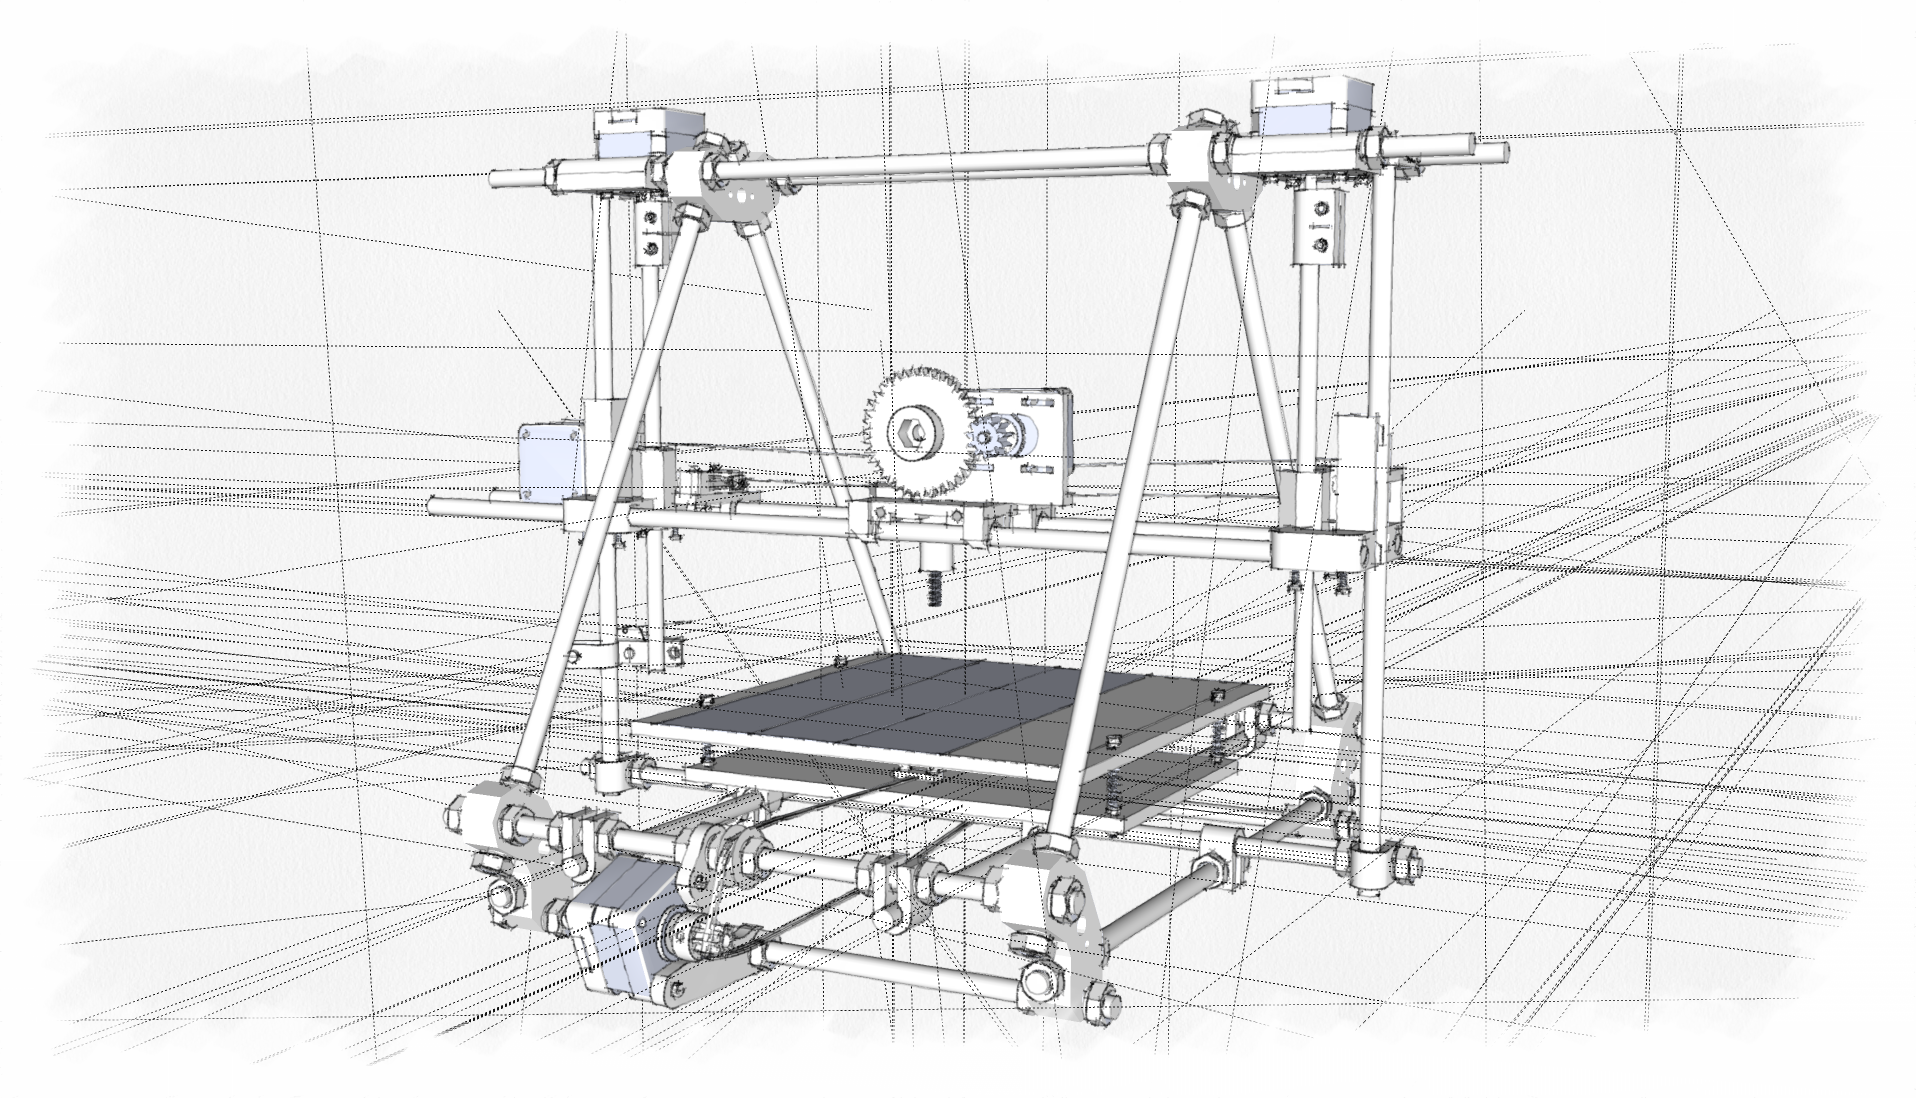
\includegraphics[width=1\linewidth]{graphics/prusa_cover.png} \vspace{\baselineskip}
			\pscharpath{\OS Visual Instructions} \vspace{\baselineskip}\vspace{\baselineskip}
			
\includegraphics[scale=0.32]{graphics/reprap_logo.png}
		\end{center}
	\end{titlingpage}

	\setcounter{tocdepth}{0}
	\tableofcontents

	\titlespacing*{\chapter}{0pt}{-20pt}{20pt}
	\pagestyle{reprap}
	\newpage
\phantomsection
\addcontentsline{toc}{chapter}{Introduction}
\chapter*{\pscharpath{\OM Introduction}}
	\hangindent=\parindent
	\textbf{Goal:}\\
		Provide a visual guide of the steps needed to construct a Prusa Mendel Printer. The\\
		instructions contained within are copied verbatim from the reprap.org wiki:\\
		http://reprap.org/wiki/Prusa as of 20th March 2011\vspace{\baselineskip}

	\noindent
	\hangindent=\parindent
	\textbf{Original Authors:}\\
		Prusajr (design),\\
		Kliment (maintenance and documentation)\vspace{\baselineskip}
	
	\noindent
	\hangindent=\parindent
	\textbf{Authors of this Document:}\\
		Gary Hodgson (http://garyhodgson.com/reprap)\\
		Brad Pitcher (http://polymaker.tumblr.com)\vspace{\baselineskip}

	\noindent
	\hangindent=\parindent
	\textbf{Mendel STL Model Files:}\\
		https://github.com/prusajr/PrusaMendel\vspace{\baselineskip}

	\noindent
	\hangindent=\parindent
	\textbf{Inspiration taken from Reprap Mendel Sketchup Model by Capo:}\\
		http://sketchup.google.com/3dwarehouse/details?mid=86dc5e3cc80958355ad914839c51e370\vspace{\baselineskip}

	\noindent
	\hangindent=\parindent
	\textbf{Sketchup Models:}\\
		Wade Geared Extruder by Capo:\\
		http://sketchup.google.com/3dwarehouse/details?mid=5e02c01a6f2c2855511146b0789315c6\vspace{\baselineskip}

	\noindent
	\hangindent=\parindent
	\textbf{Licensing:}\\
		\textbf{Prusa Mendel:} GPL (http://reprap.org/wiki/GPL)\\
		\textbf{This Document:} GFDL (http://www.gnu.org/licenses/fdl.html)\vspace{\baselineskip}

	\vspace{\baselineskip}
	\vspace{\baselineskip}
	\vspace{\baselineskip}
	\vspace{\baselineskip}

	\noindent
	\hangindent=\parindent
	The source files for this document available on Github:\\
		https://github.com/brad/prusa\_mendel\_visual\_instructions\vspace{\baselineskip}

	\noindent
	\hangindent=\parindent
	Issues with this document can be submitted on the Github project page:\\
		https://github.com/brad/prusa\_mendel\_visual\_instructions/issues

	\newpage
\phantomsection
\addcontentsline{toc}{chapter}{Changelog}
\chapter*{\pscharpath{\OM Changelog}}

V1 - 20th March 2011\\
Initial Version\\
V2 - 27th March 2011\\
Issue \#1: (z-motor-holder nuts on p60) - Alternative added Part 8 Step 5\\
Issue \#2: (Footed vertices missing the foot) - Comment added Part 1 Step 6\\
Issue \#3: (Suggestions from TianChang) - Comment added to Part 8 Step 13 \& 19\\
Issue \#6: (x axis smooth rods) - Comment added to Part 9 Step 5; Images
updated\\
Issue numbers referenced from the Github project page:\\
https://github.com/garyhodgson/prusa\_mendel\_visual\_instructions/issues\\


	\chapterstyle{outlinechapter}
	\pagestyle{headings}
	\headsep=20pt
	\chapter{Assembling the frame vertex triangles}
	\section{}
	Take one of the 370mm threaded rods, and slip an M8 washer onto the middle of
	it. \\
	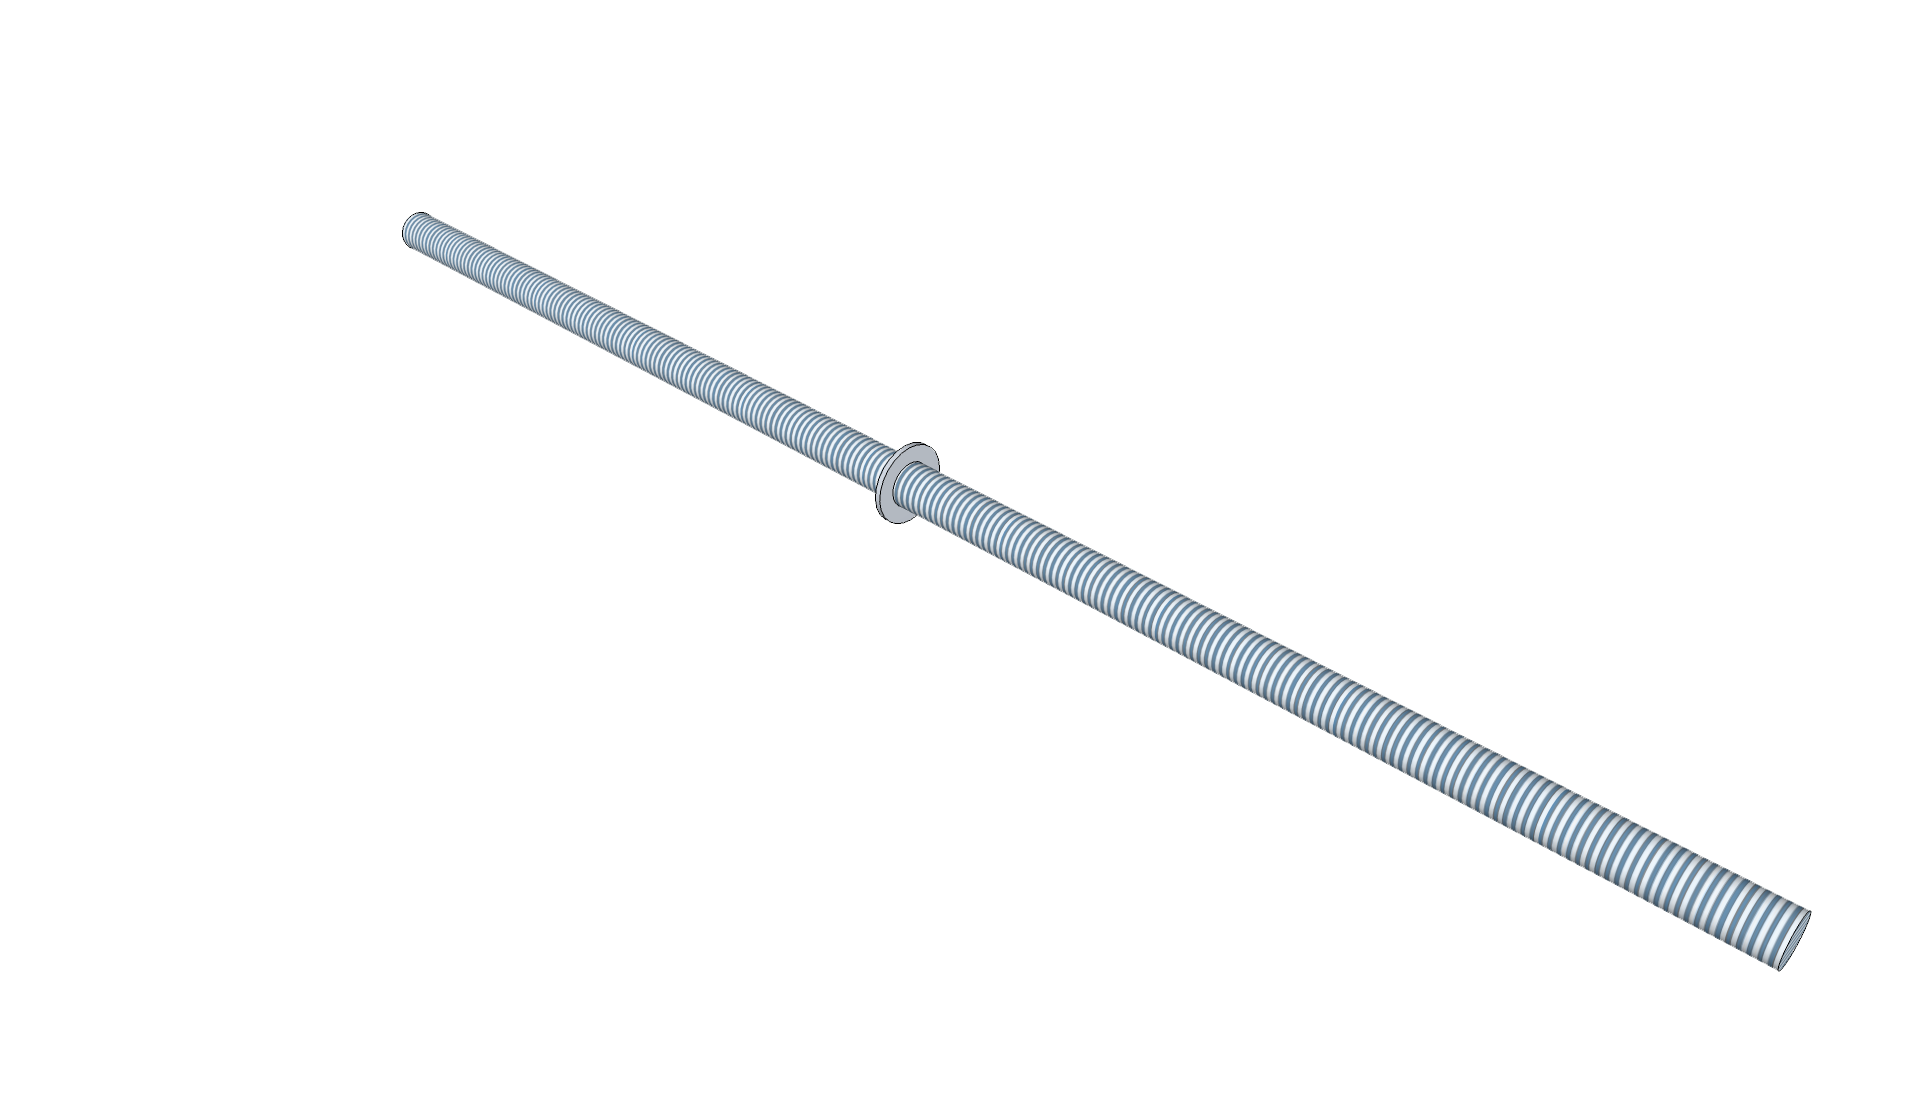
\includegraphics[width=1\linewidth]{graphics/ch1_1.png}
	
	\section{}
	Take the RP bar clamp (the U-shaped bit with the two holes) and slide the threaded rod through the two
	holes until the clamp sits next to the washer. \\
	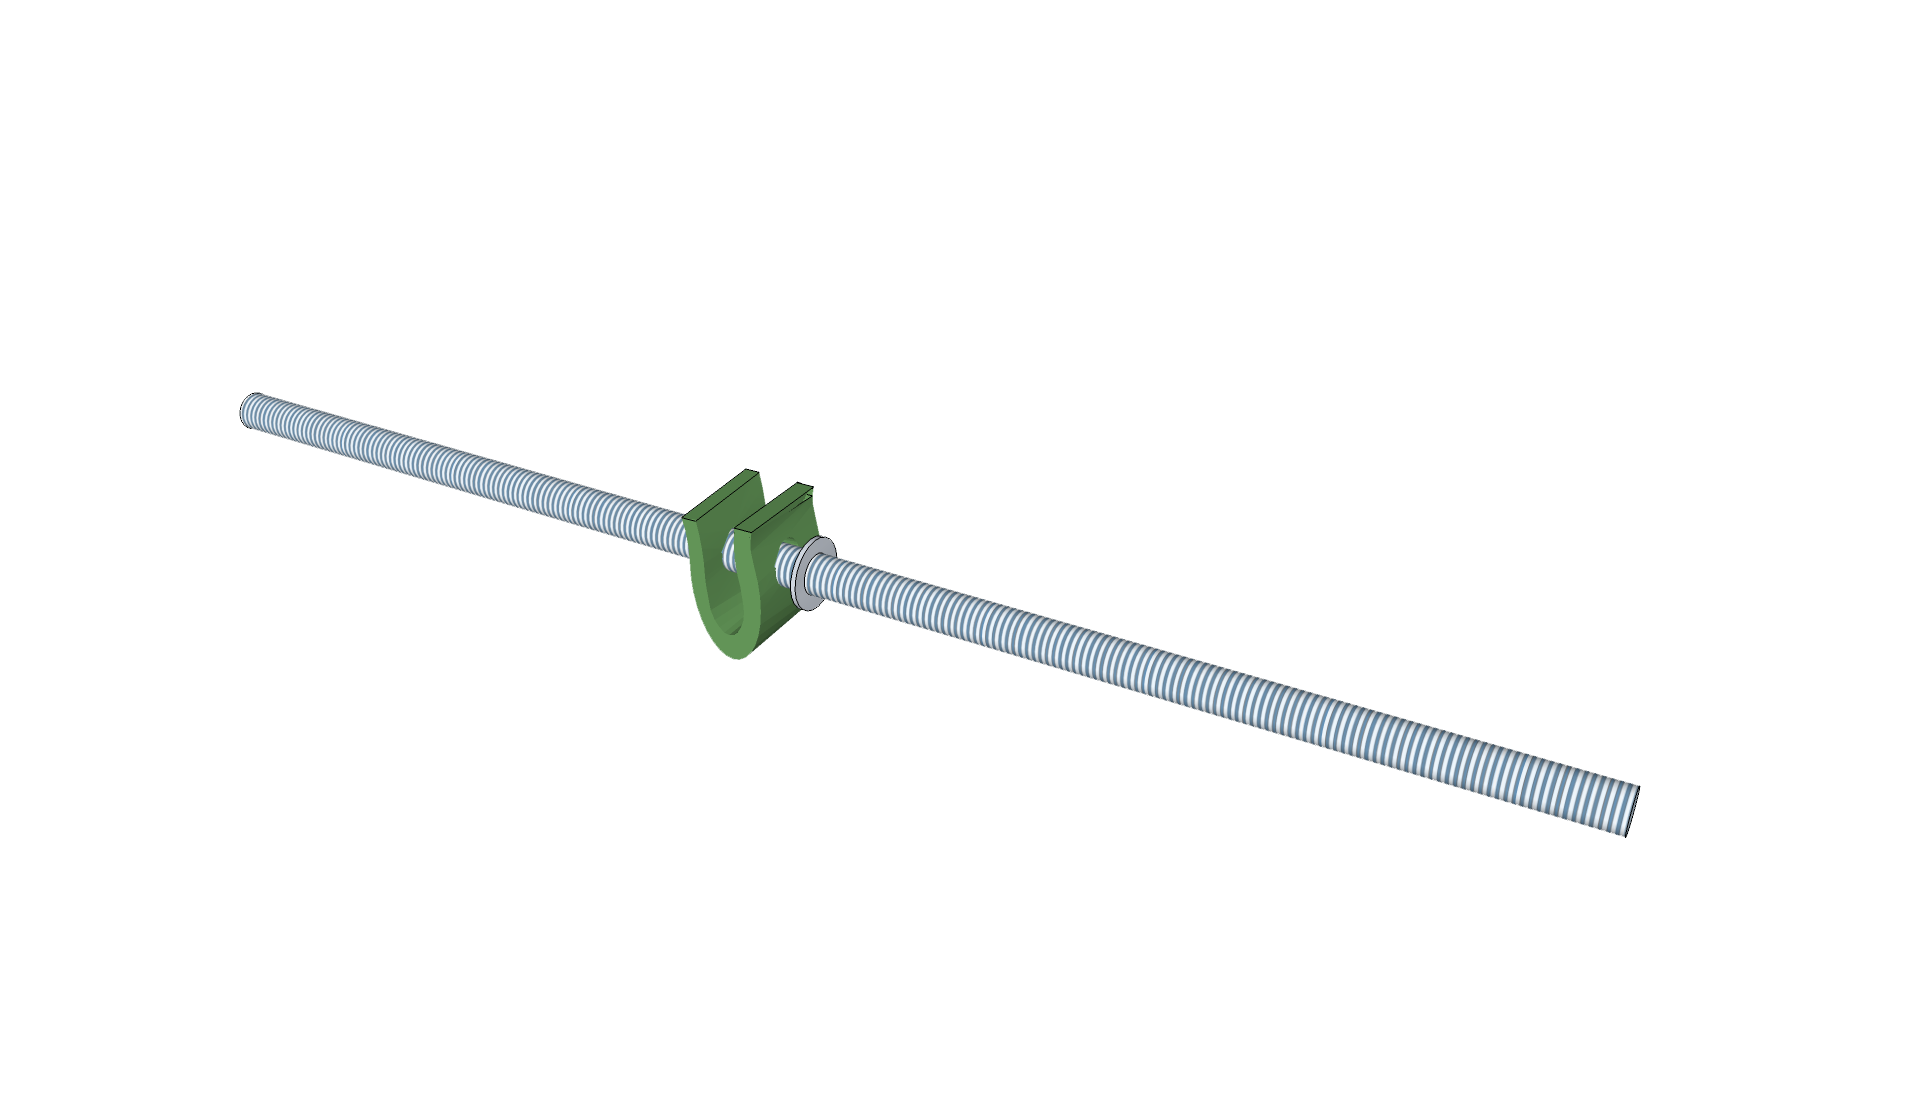
\includegraphics[width=1\linewidth]{graphics/ch1_2.png}
	
	\section{}
	Slide another washer onto the rod from the other side. \\
	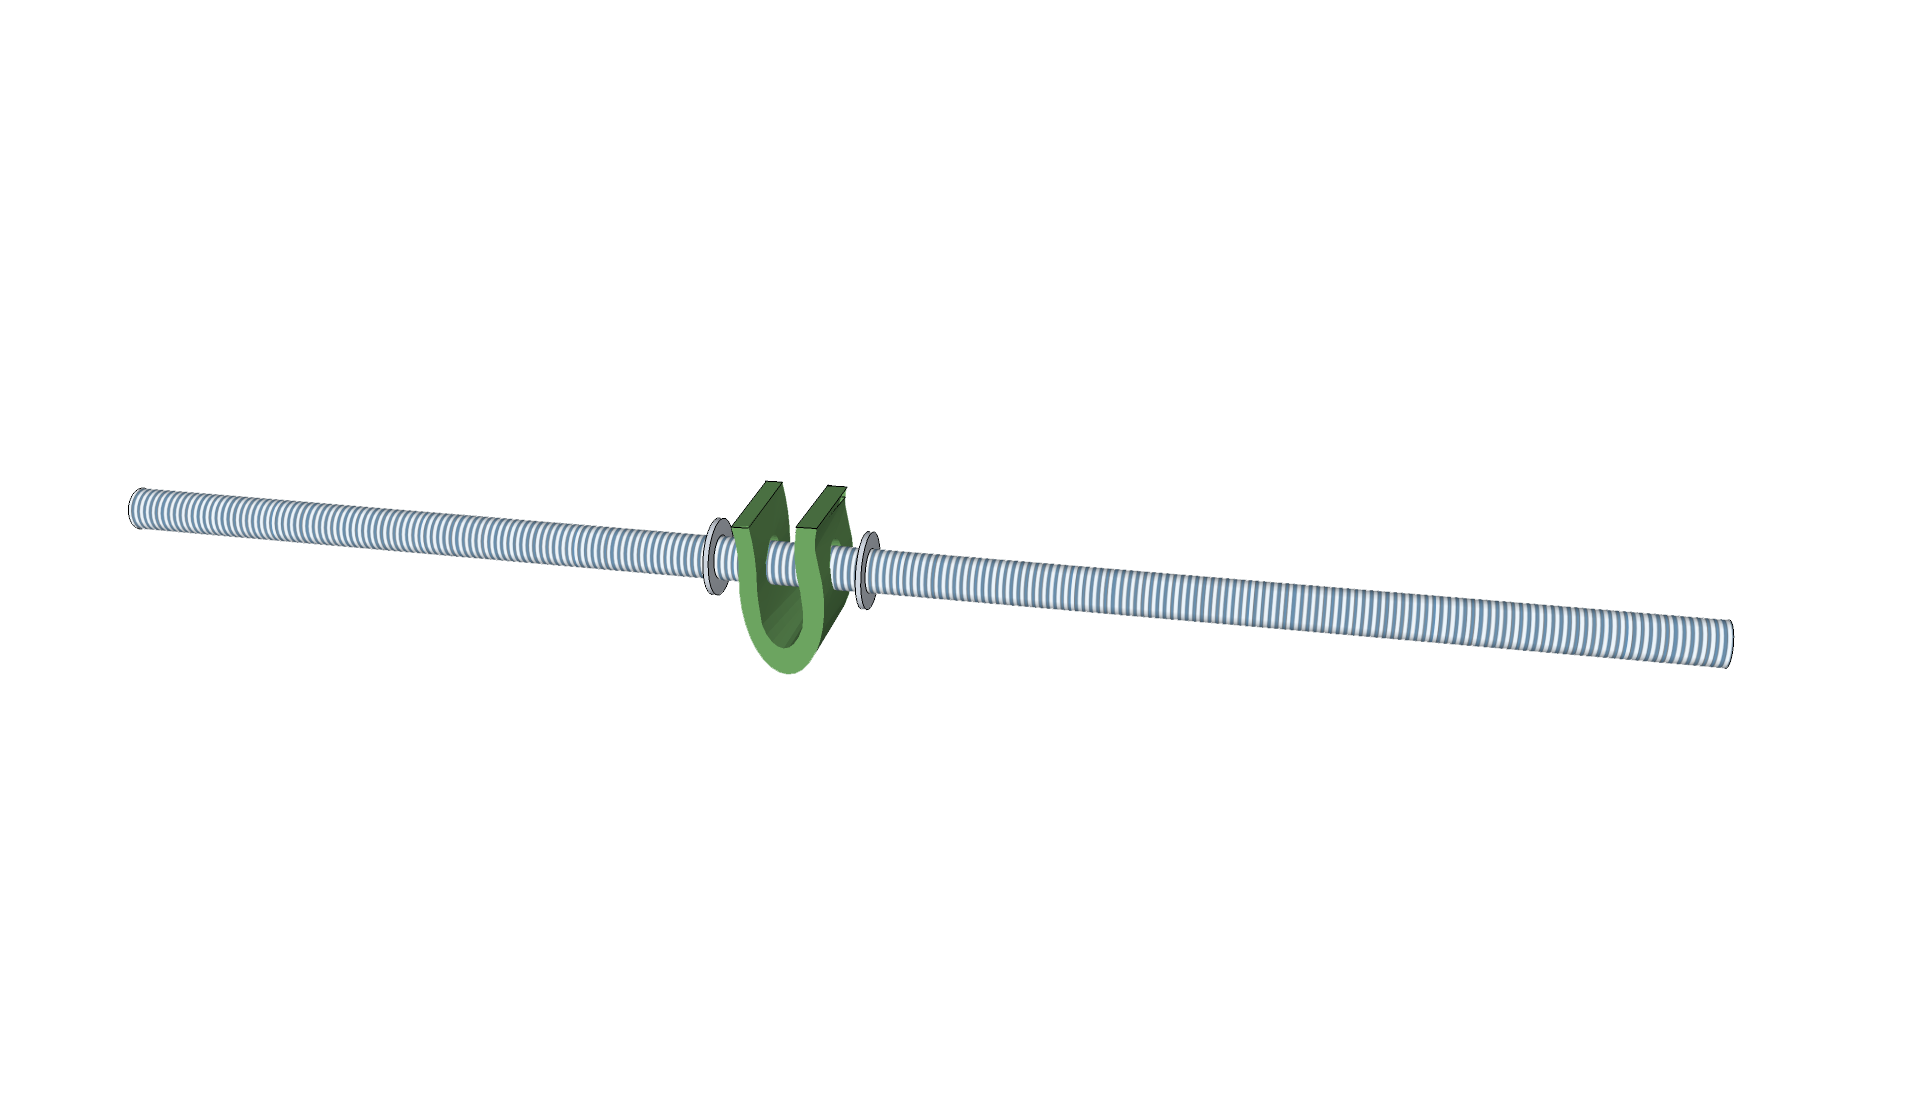
\includegraphics[width=1\linewidth]{graphics/ch1_3.png}
	
	\section{}
	Thread two M8 nuts onto either side of the clamp, until they are next to the washer, but do not tighten
	them yet. \\
	\begin{overpic}[width=1\linewidth]{graphics/ch1_4_1.png}
		\put(0,0){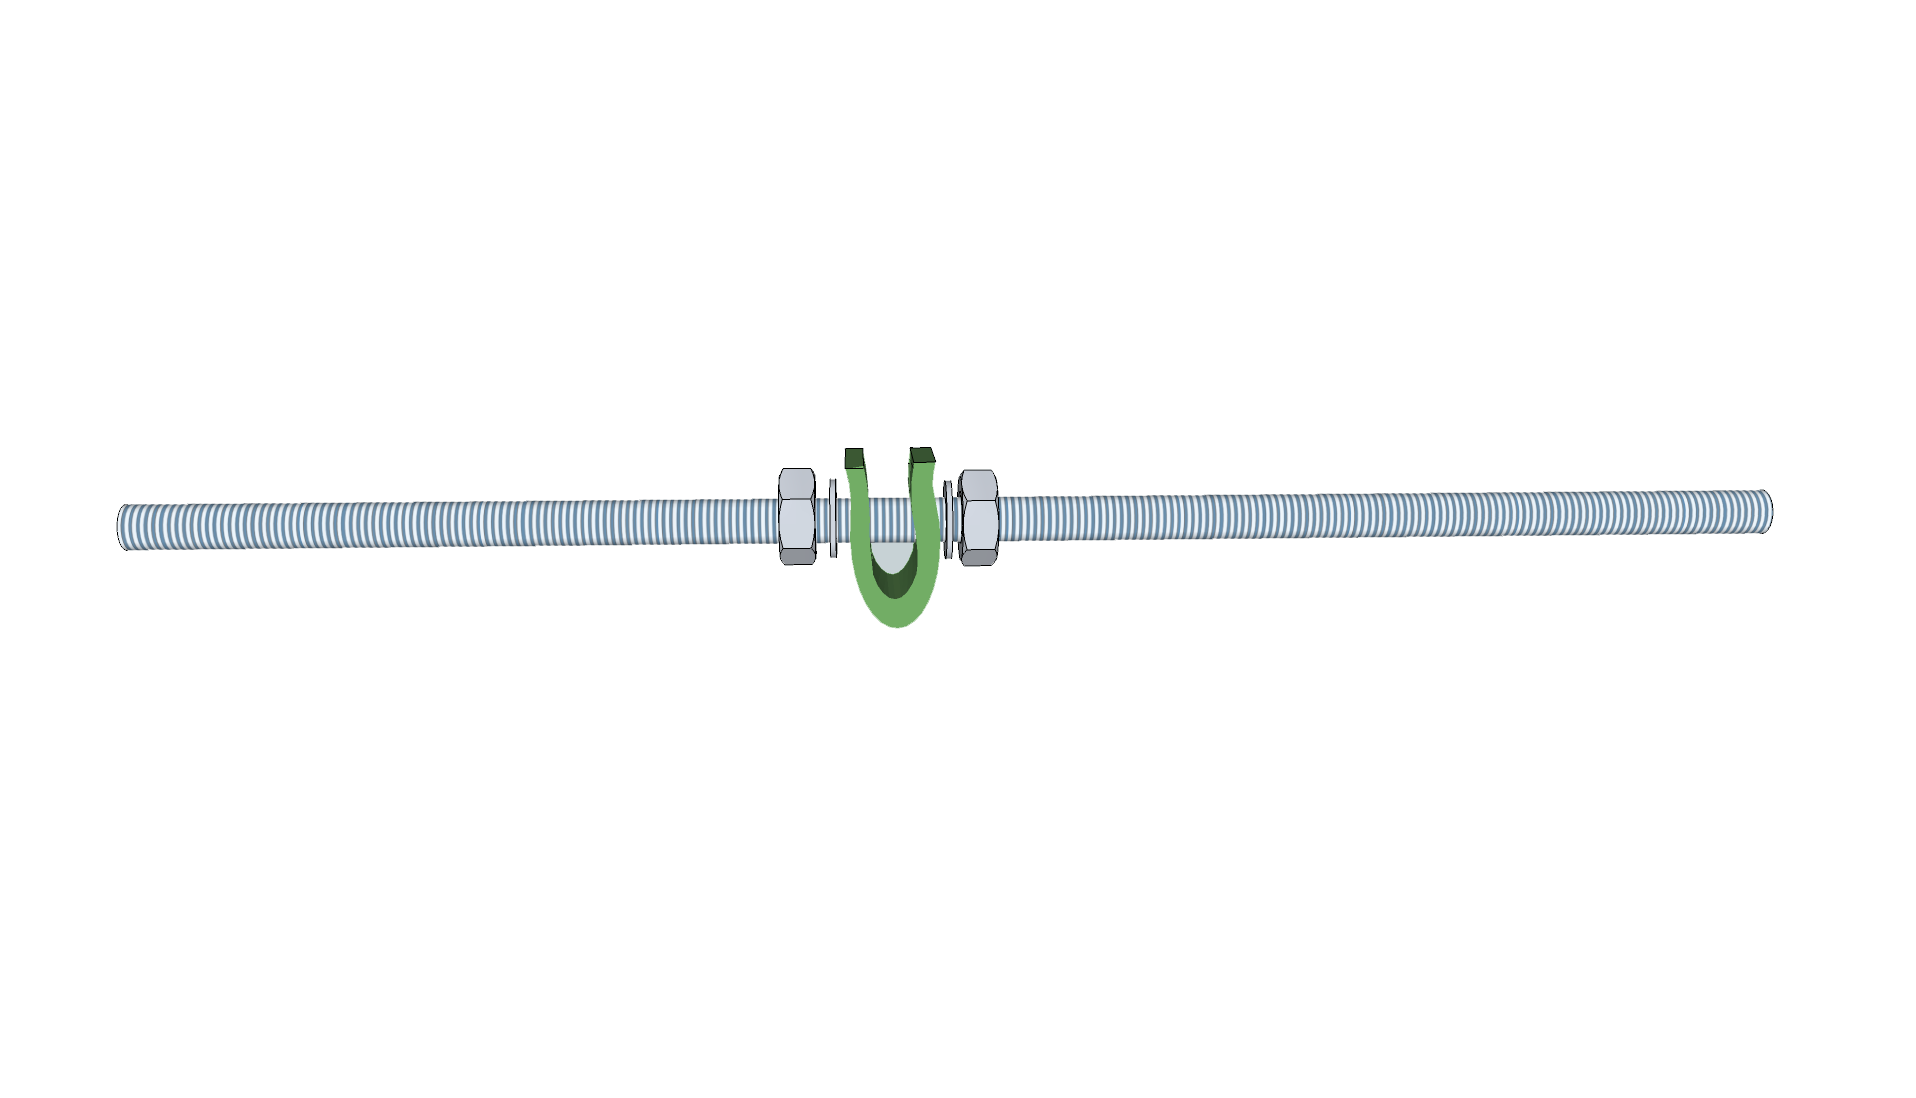
\includegraphics[width=0.4\linewidth]{graphics/ch1_4_2.png}}
	\end{overpic}
	
	\section{}
	Thread another two nuts on each side of the rod, followed by washers. See the picture for what it
	should look like. \\
	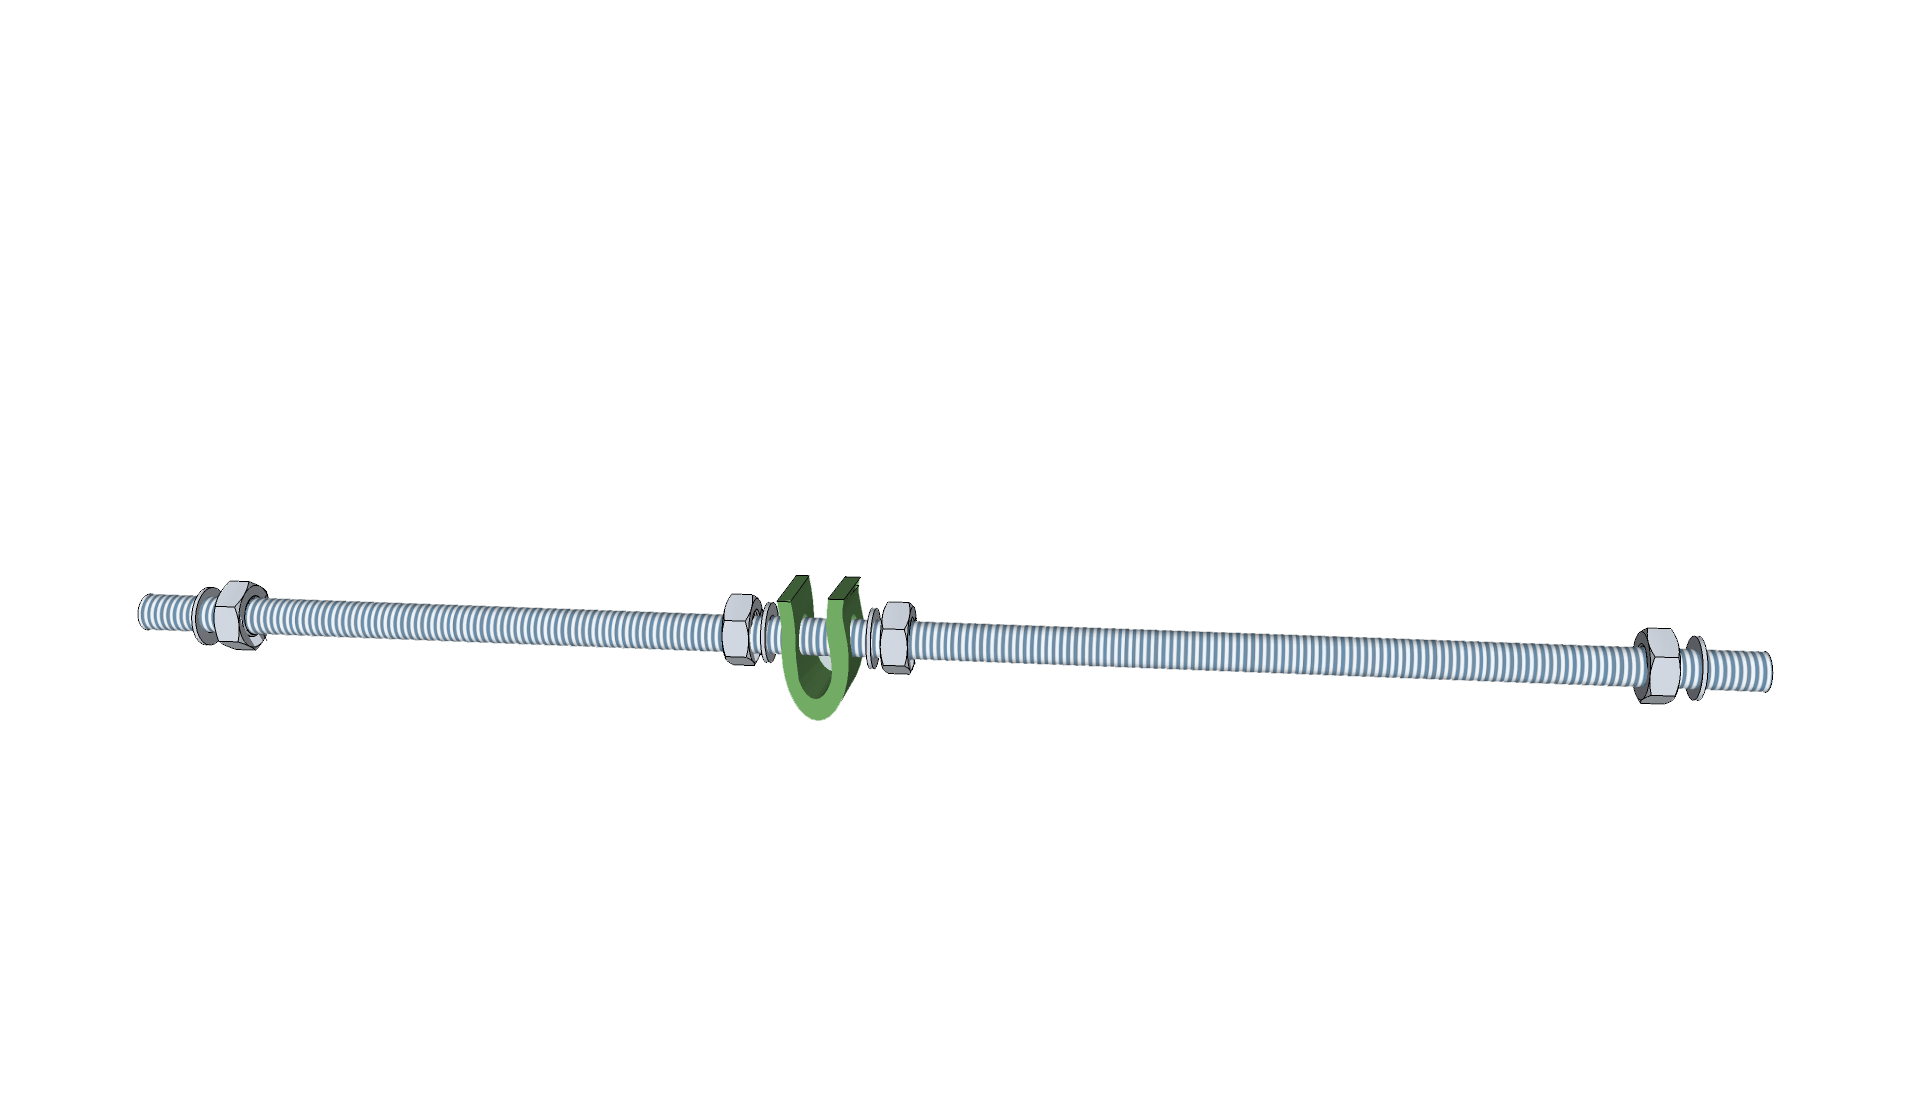
\includegraphics[width=1\linewidth]{graphics/ch1_5.png}
	
	\section{}
	Slide the rod through the long bottom (footed) side of two vertices. Make sure the feet point in the same
	direction. Also make sure the bulge on the non-footed side of the vertex points
	outwards. \\
	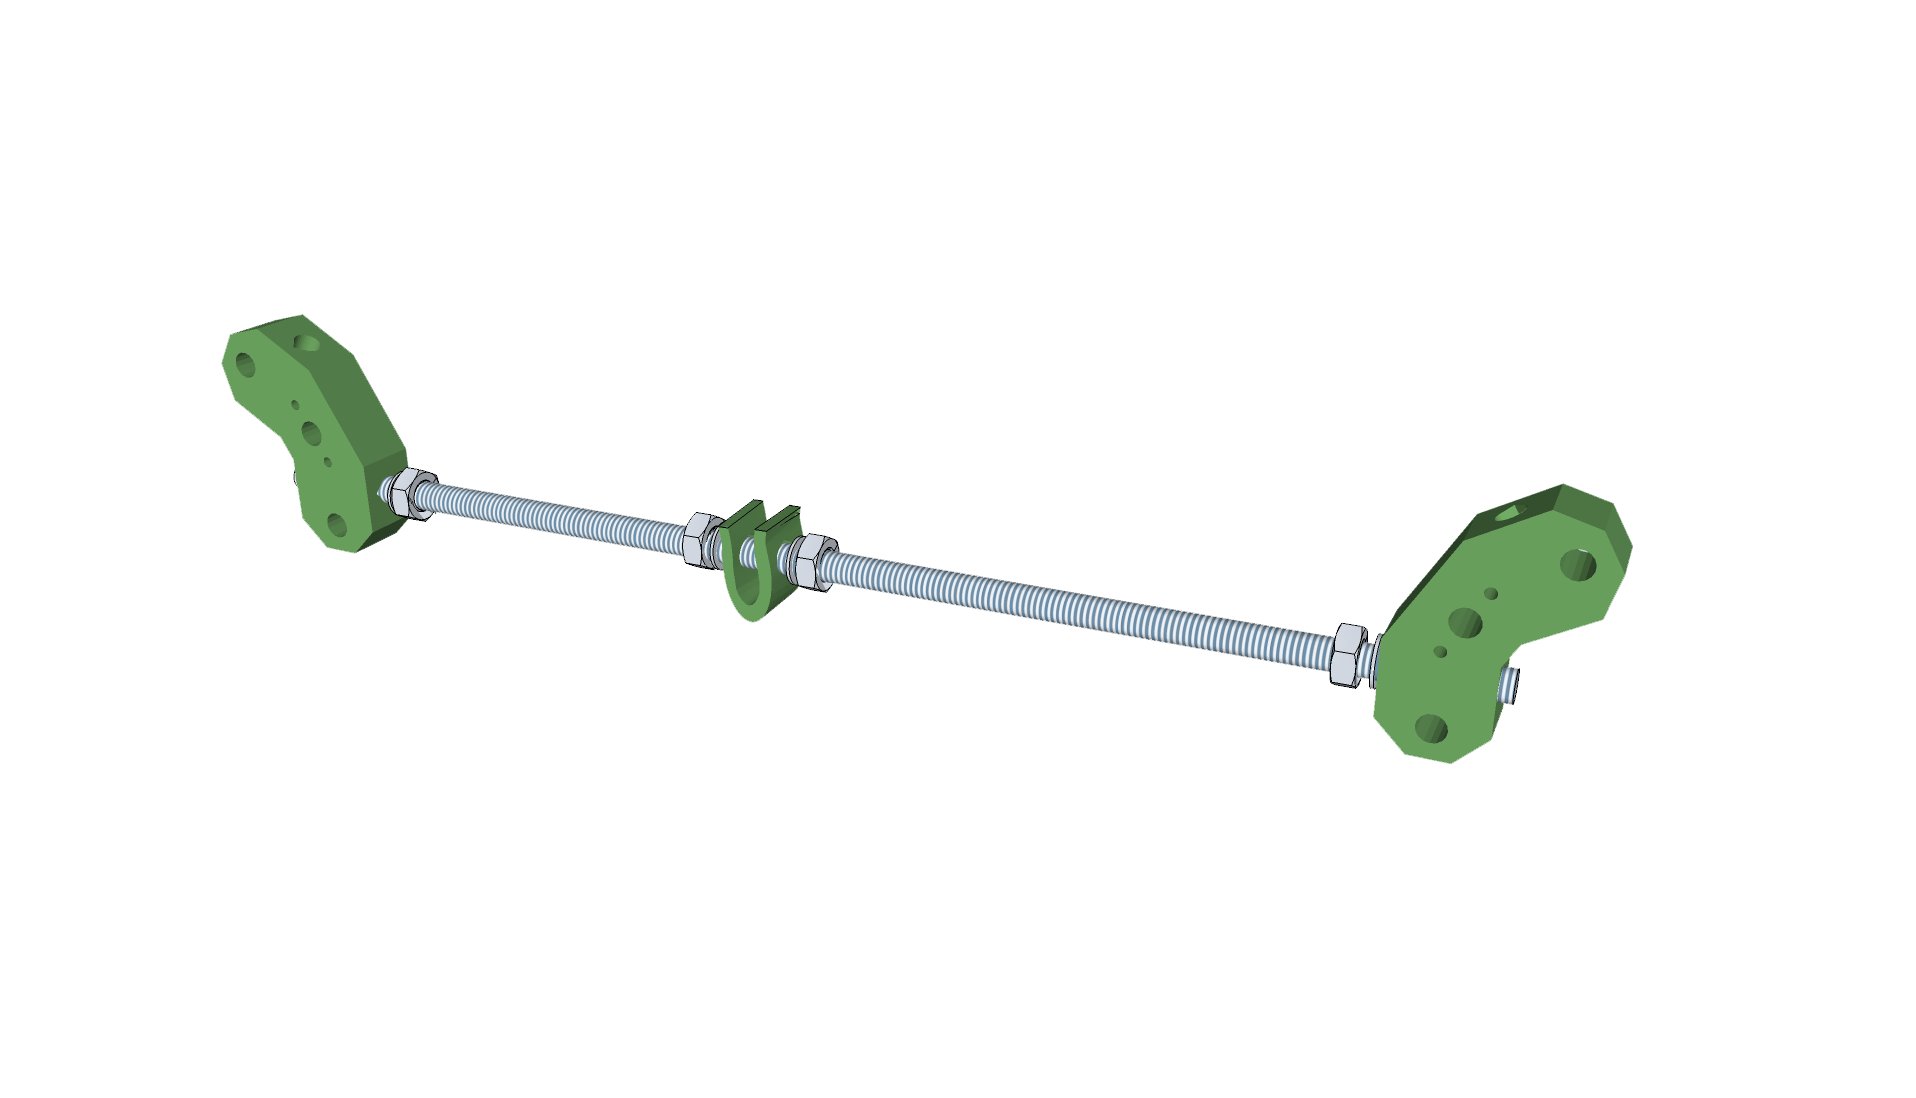
\includegraphics[width=1\linewidth]{graphics/ch1_6_1.png} \\
	You can use either footed or non-footed vertices to build this (the footed ones
	look better, but are not critical.) \\
	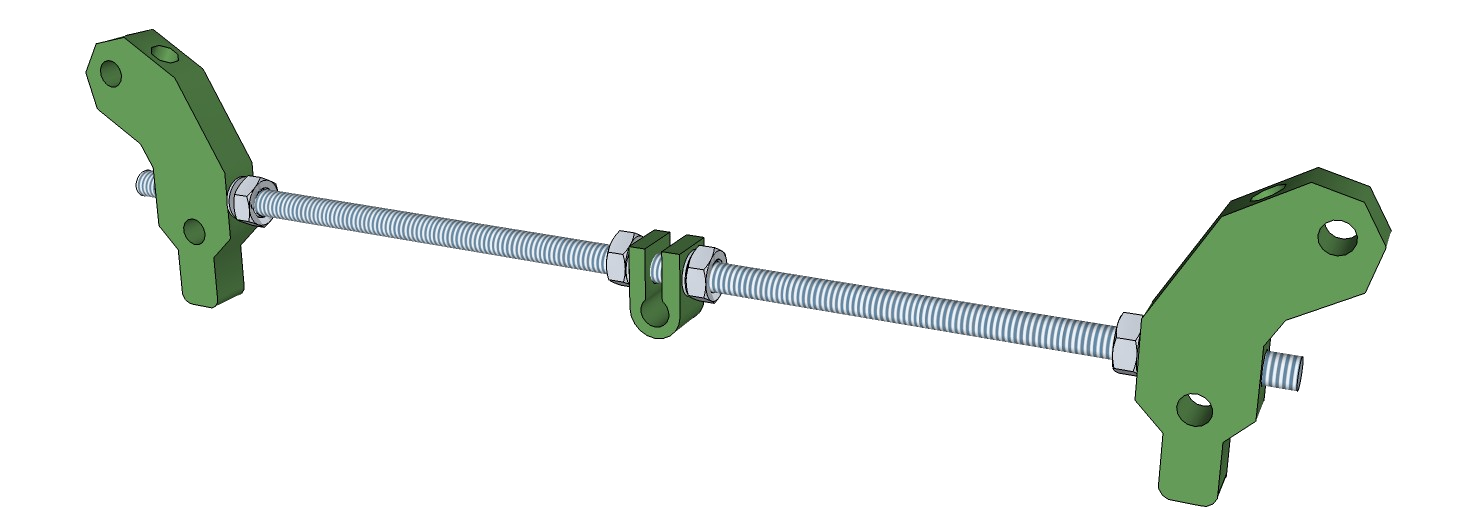
\includegraphics[width=1\linewidth]{graphics/ch1_6_2.png}
	
	\section{}
	Measure the distance. The distance between the two vertices should be 290mm (along the rod,
	equivalent is 11-13/32"). Get it approximately right now, we will check this again later. If you have a
	frame jig, place it between the two vertices and adjust the nuts until you can just barely fit the jig J1
	between them. \\
	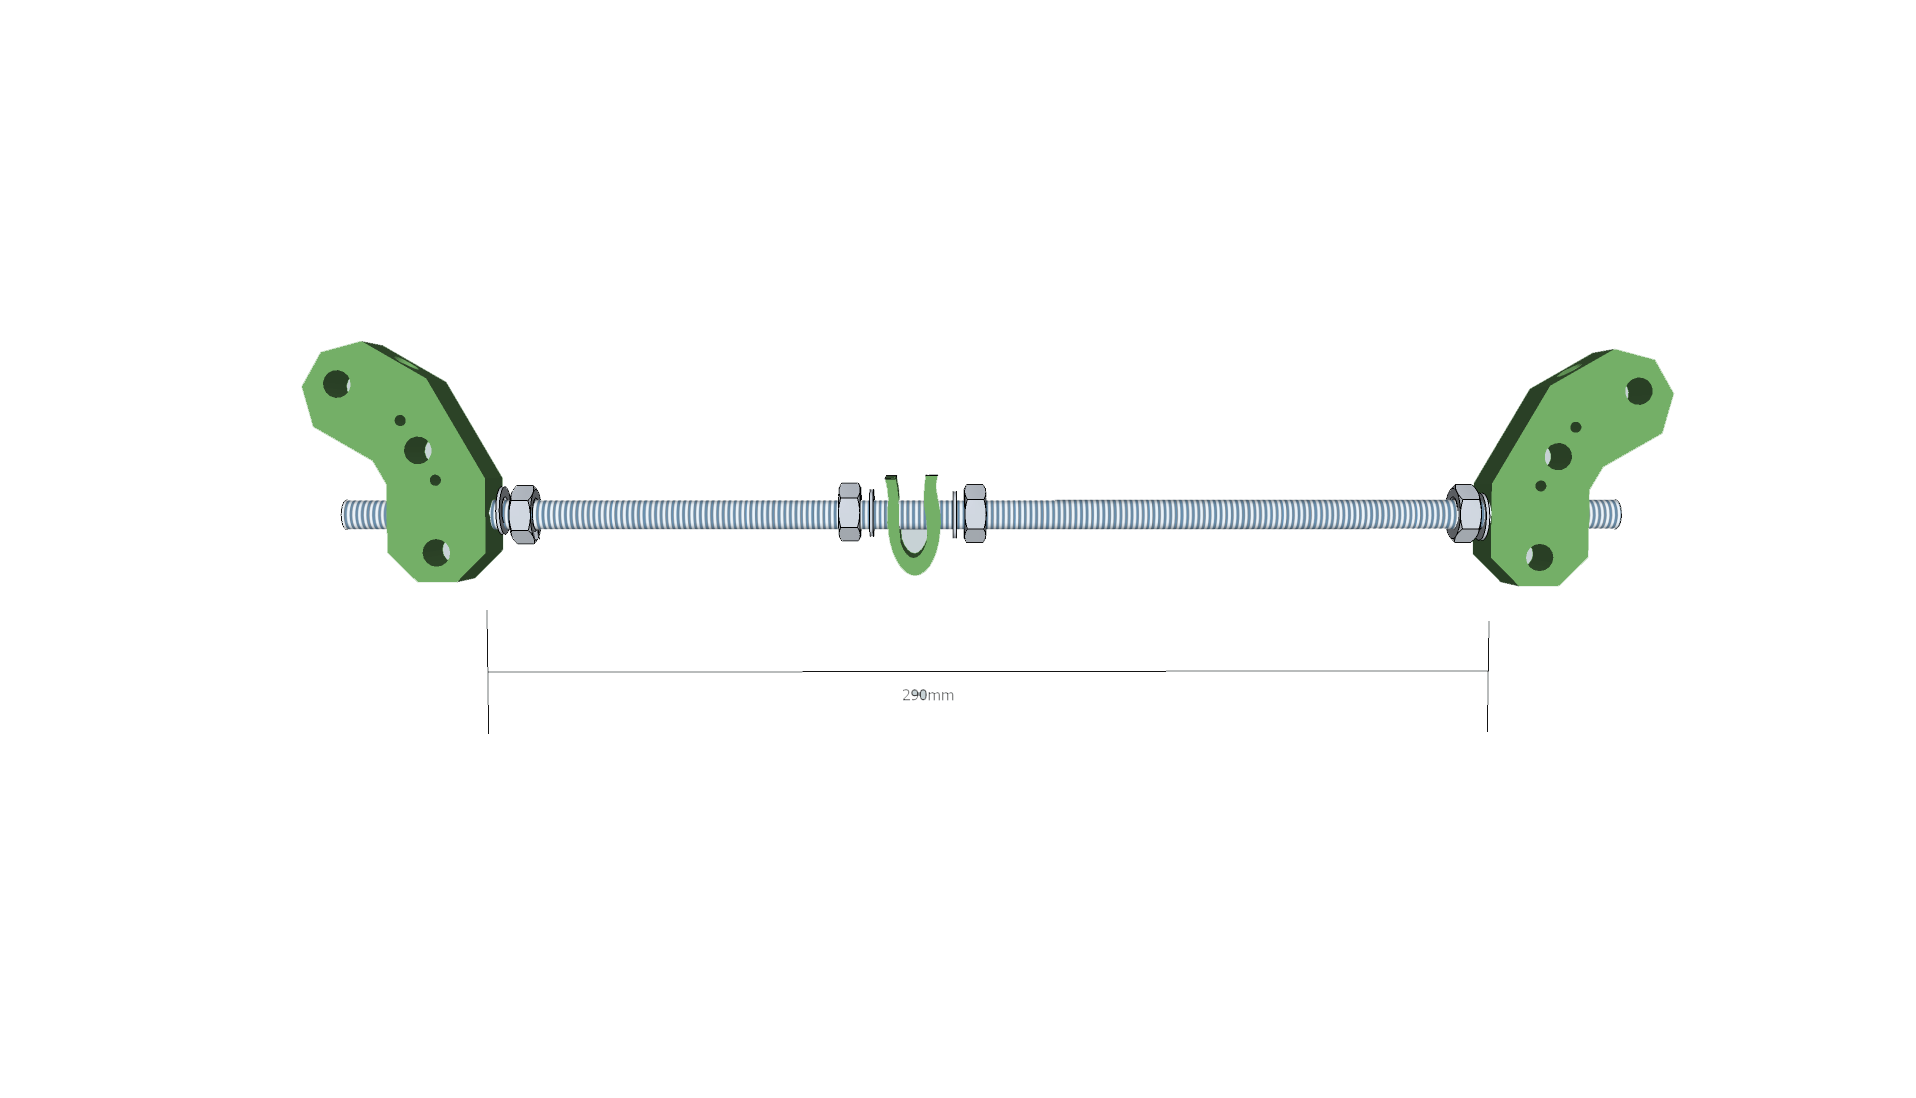
\includegraphics[width=1\linewidth]{graphics/ch1_7.png}
	
	\section{}
	Place another washer and nut on the other side of the vertex. Tighten, but not too much. We'll need a
	bit of flexibility here still. \\
	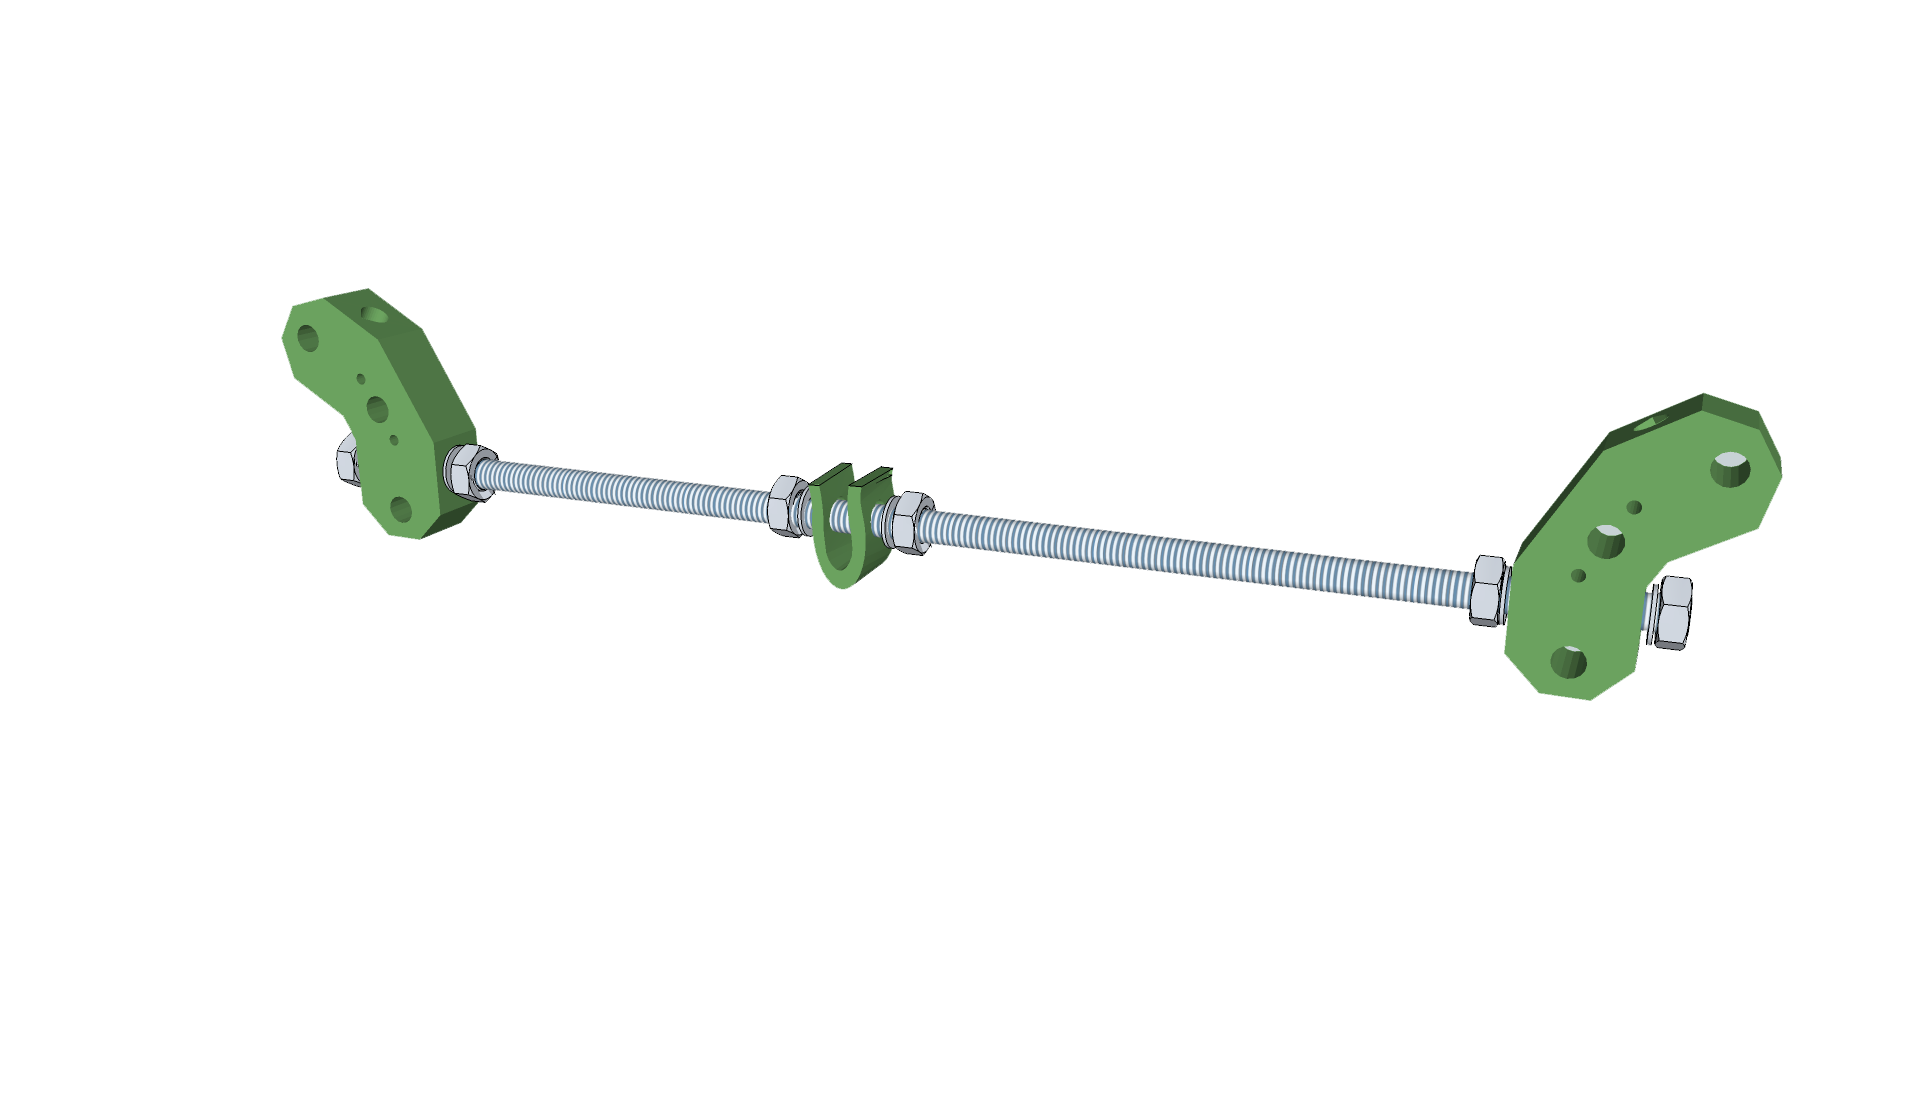
\includegraphics[width=1\linewidth]{graphics/ch1_8.png}
	
	\section{}
	Take another 370mm M8 threaded rod and place a nut followed by a washer at each
	end. \\
	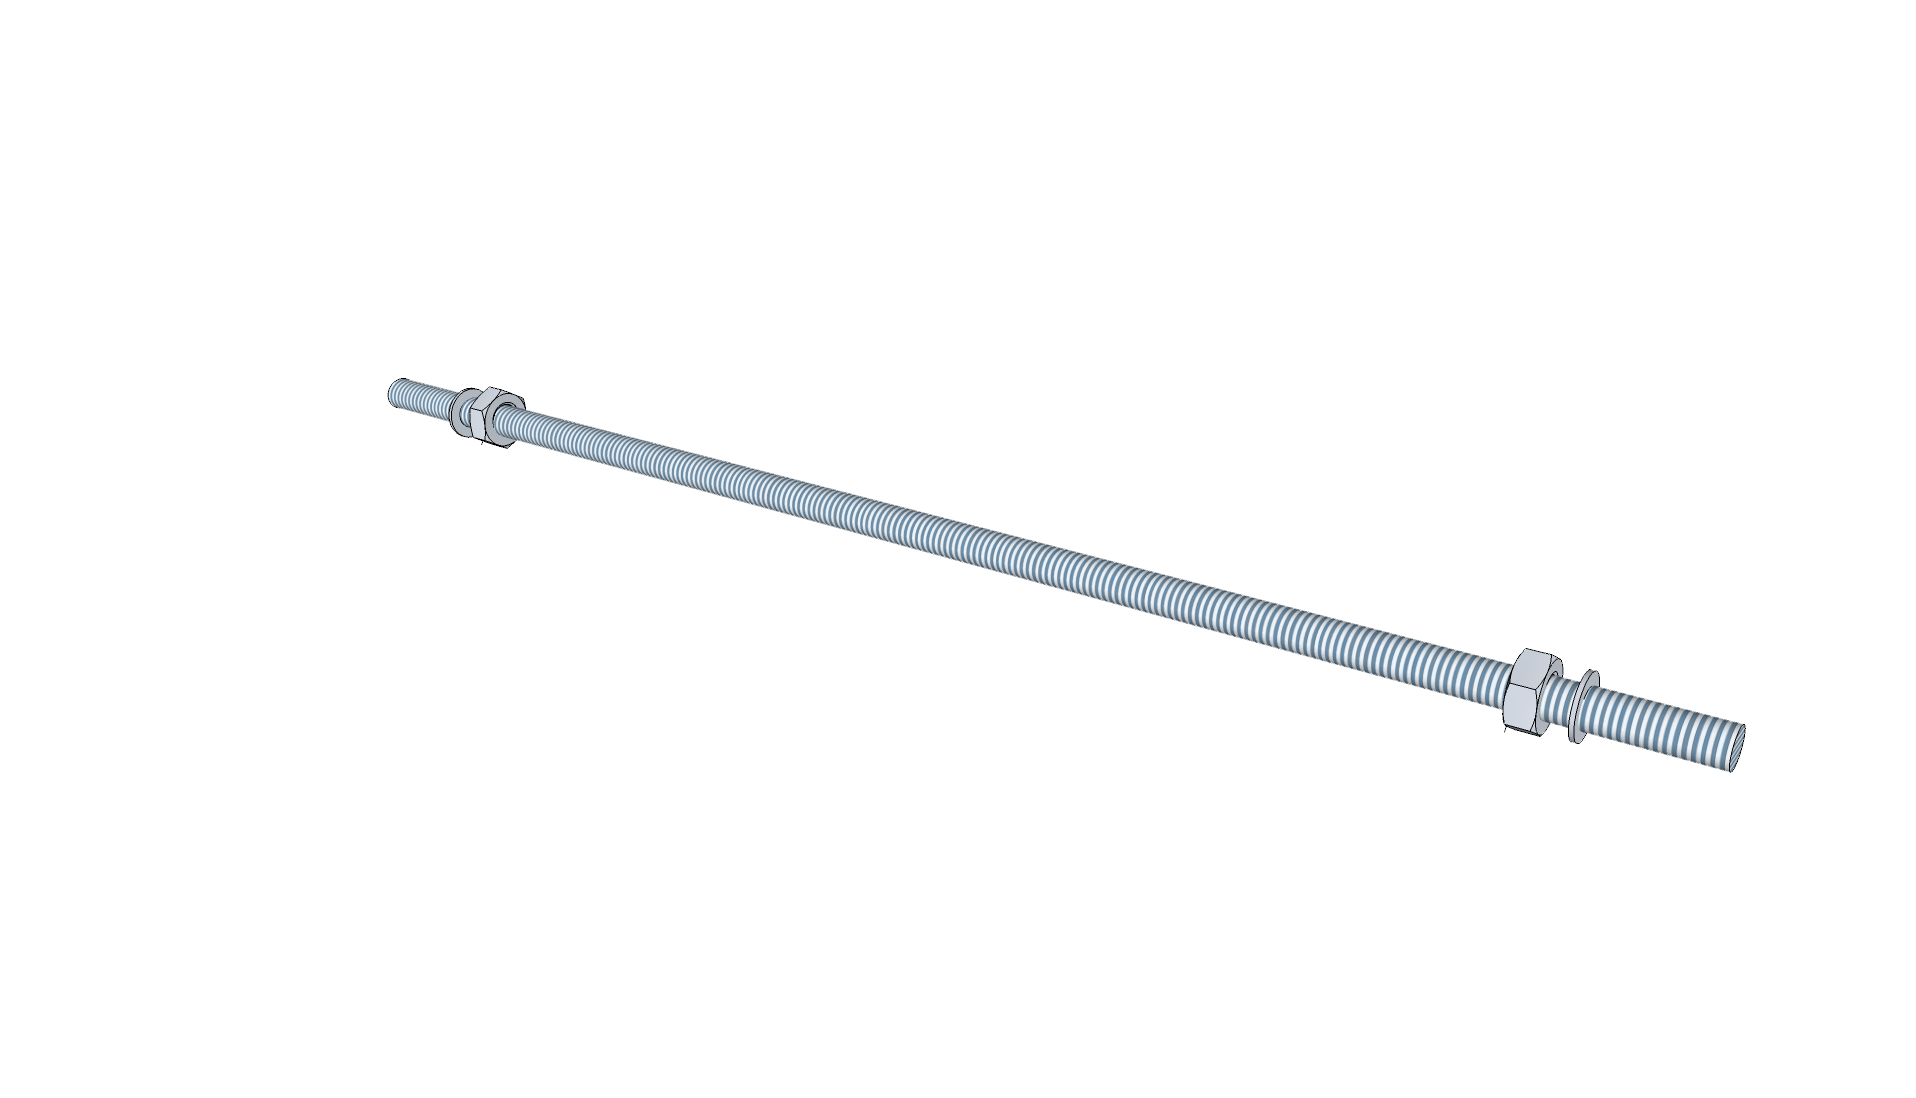
\includegraphics[width=1\linewidth]{graphics/ch1_9.png}
	
	\section{}
	Place one end of the threaded rod into the one of the two footed frame vertices. It should be in the
	same plane as the first threaded rod. Fix it in place with a washer and nut. You should now have two
	sides of the equilateral triangle.\\
	\begin{center}
		\begin{overpic}[width=1\linewidth]{graphics/ch1_10_1.png}
			\put(62,30){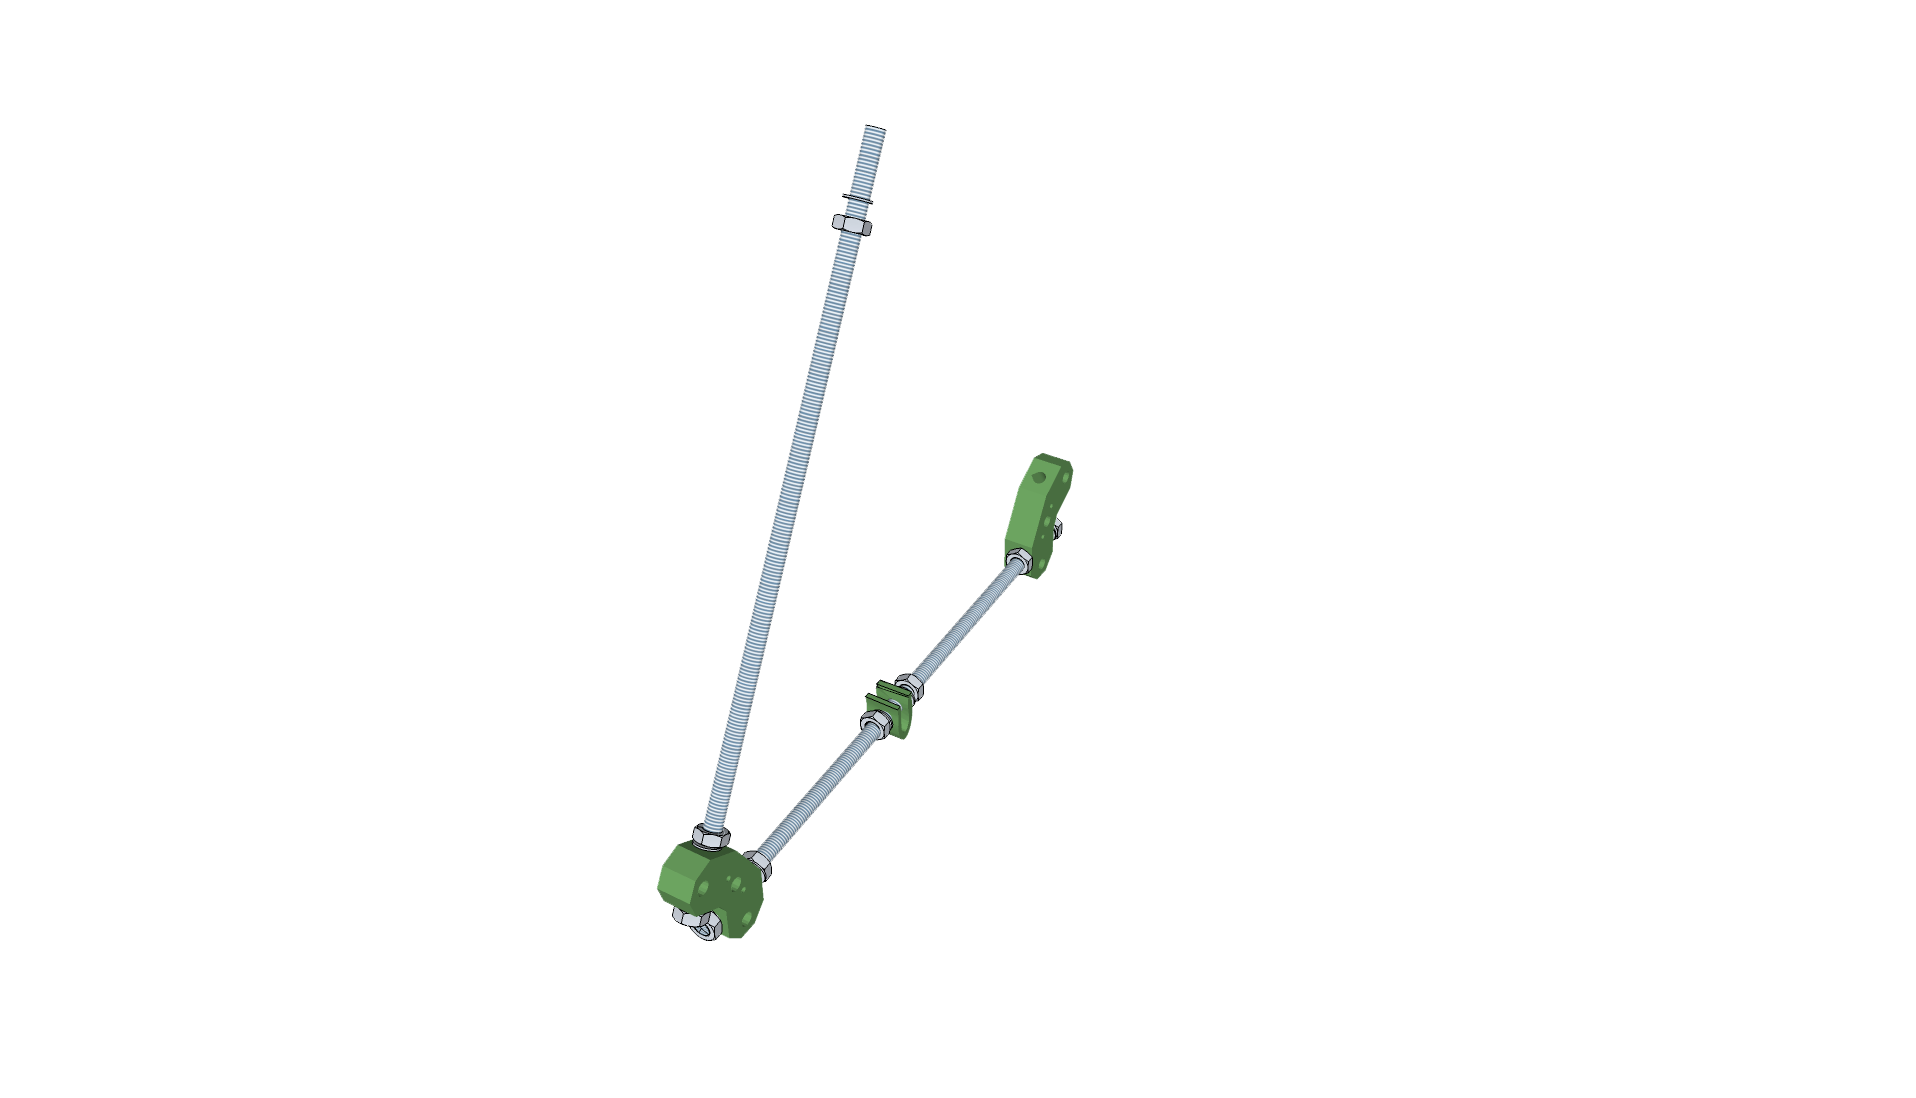
\includegraphics[width=0.5\linewidth]{graphics/ch1_10_2.png}}
		\end{overpic}
	\end{center}
	
	\section{}
	Take the third piece of threaded rod and put a nut and washer on each end. Place it in the other footed
	vertex and fix it in place with a washer and nut. You should now have a triangle of threaded rods with
	two footed vertices on two of the corners, nothing in the third corner, and a bar clamp between the two
	vertices. \\
	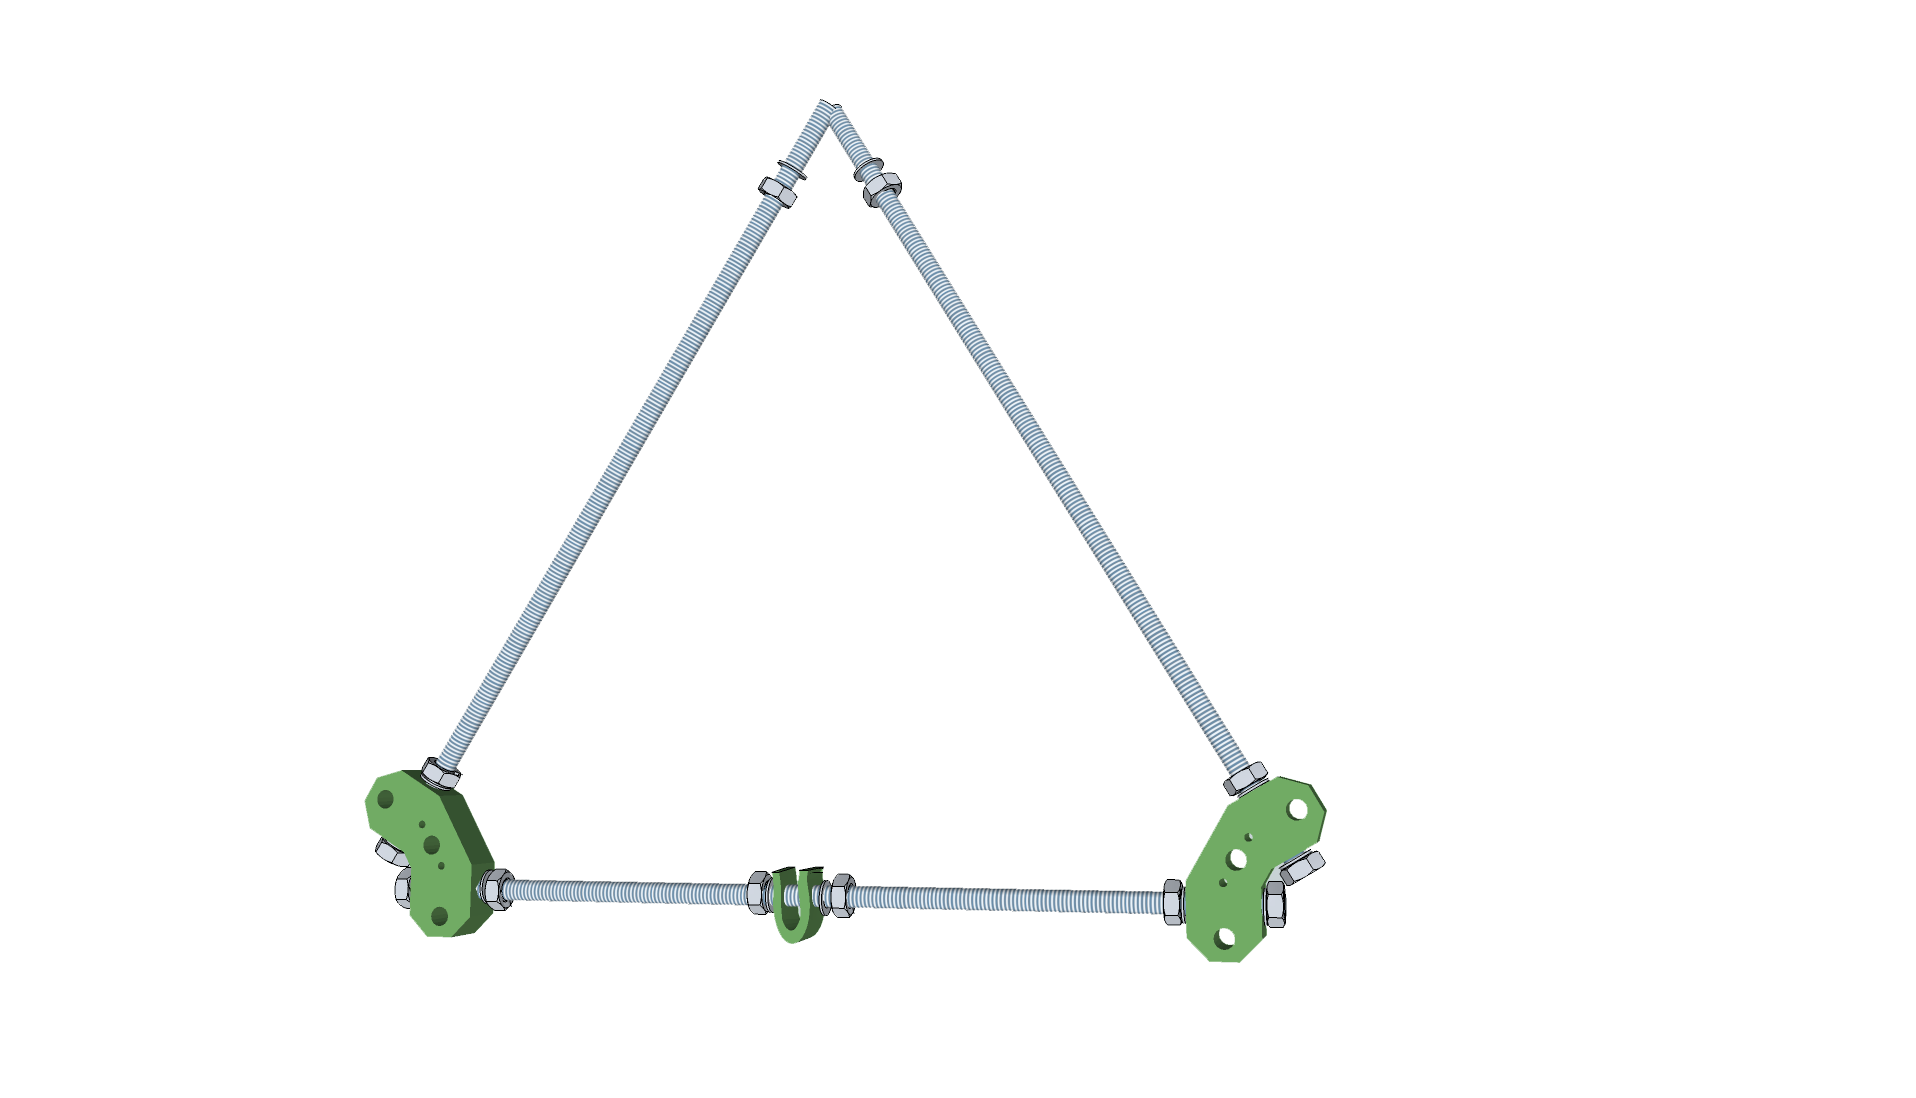
\includegraphics[width=1\linewidth]{graphics/ch1_11.png}
	
	\section{}
	Take the third vertex (non-footed) and slide it onto the threaded rods in the final corner of the triangle.
	Measure the lenghts of the three sides to make sure they are all 290mm long (along the rod from plastic
	part to plastic part, equivalent is 11-13/32"). Adjust the nuts to make sure this is so. Use the frame jig J1
	if you have one. Once done, place a washer and nut on the top of the vertex.
	Tighten all the outer nuts. \\
	\begin{center}
		\begin{overpic}[width=1\linewidth]{graphics/ch1_12_1.png}
			\put(62,30){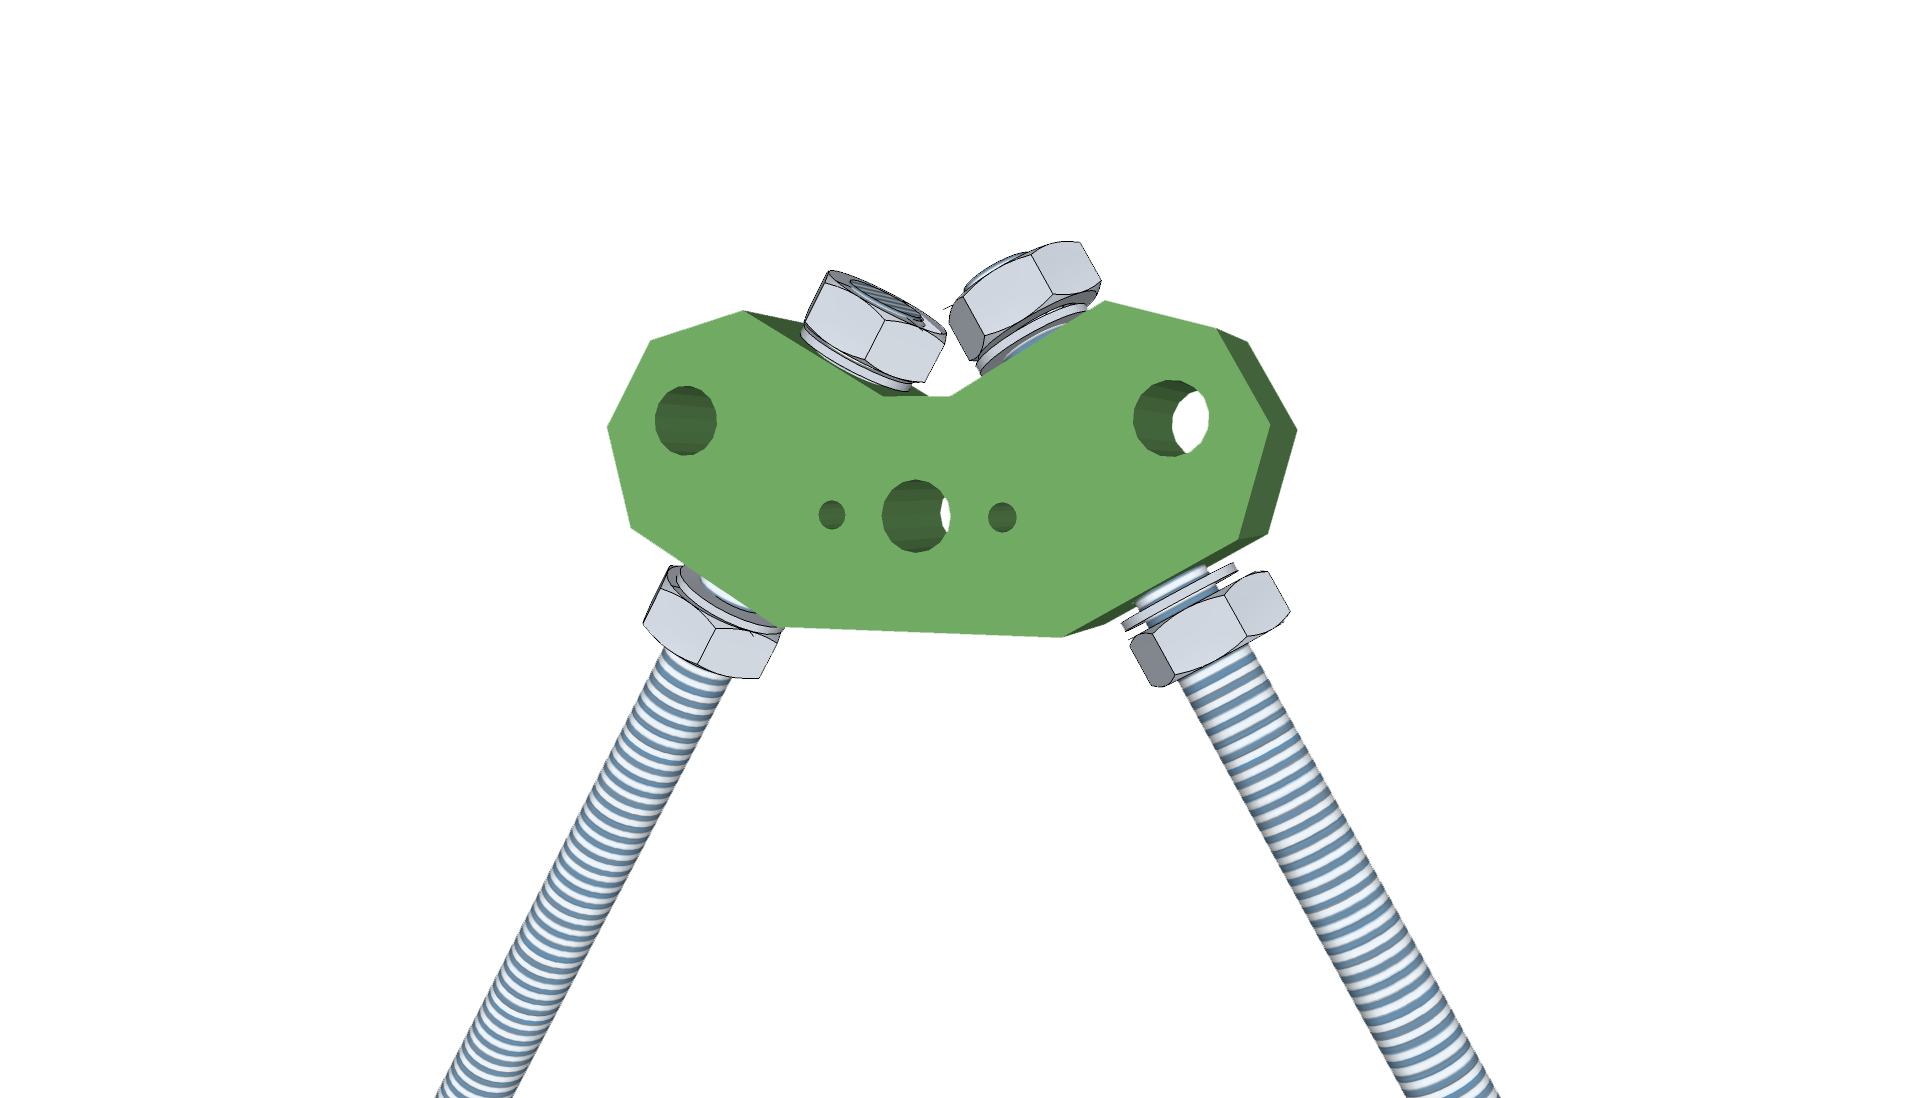
\includegraphics[width=0.5\linewidth]{graphics/ch1_12_2.png}}
		\end{overpic}
	\end{center}
	
	\section{}
	You should now have a sturdy triangle with equal-length sides, two feet on the bottom, and a bar clamp
	between the feet. Adjust the nuts around the bar clamp (but do not crush the bar clamp together yet)
	until it's approximately in the middle of the rod. Leave the nuts there loose. See photo for what you
	should have at this point. \\
	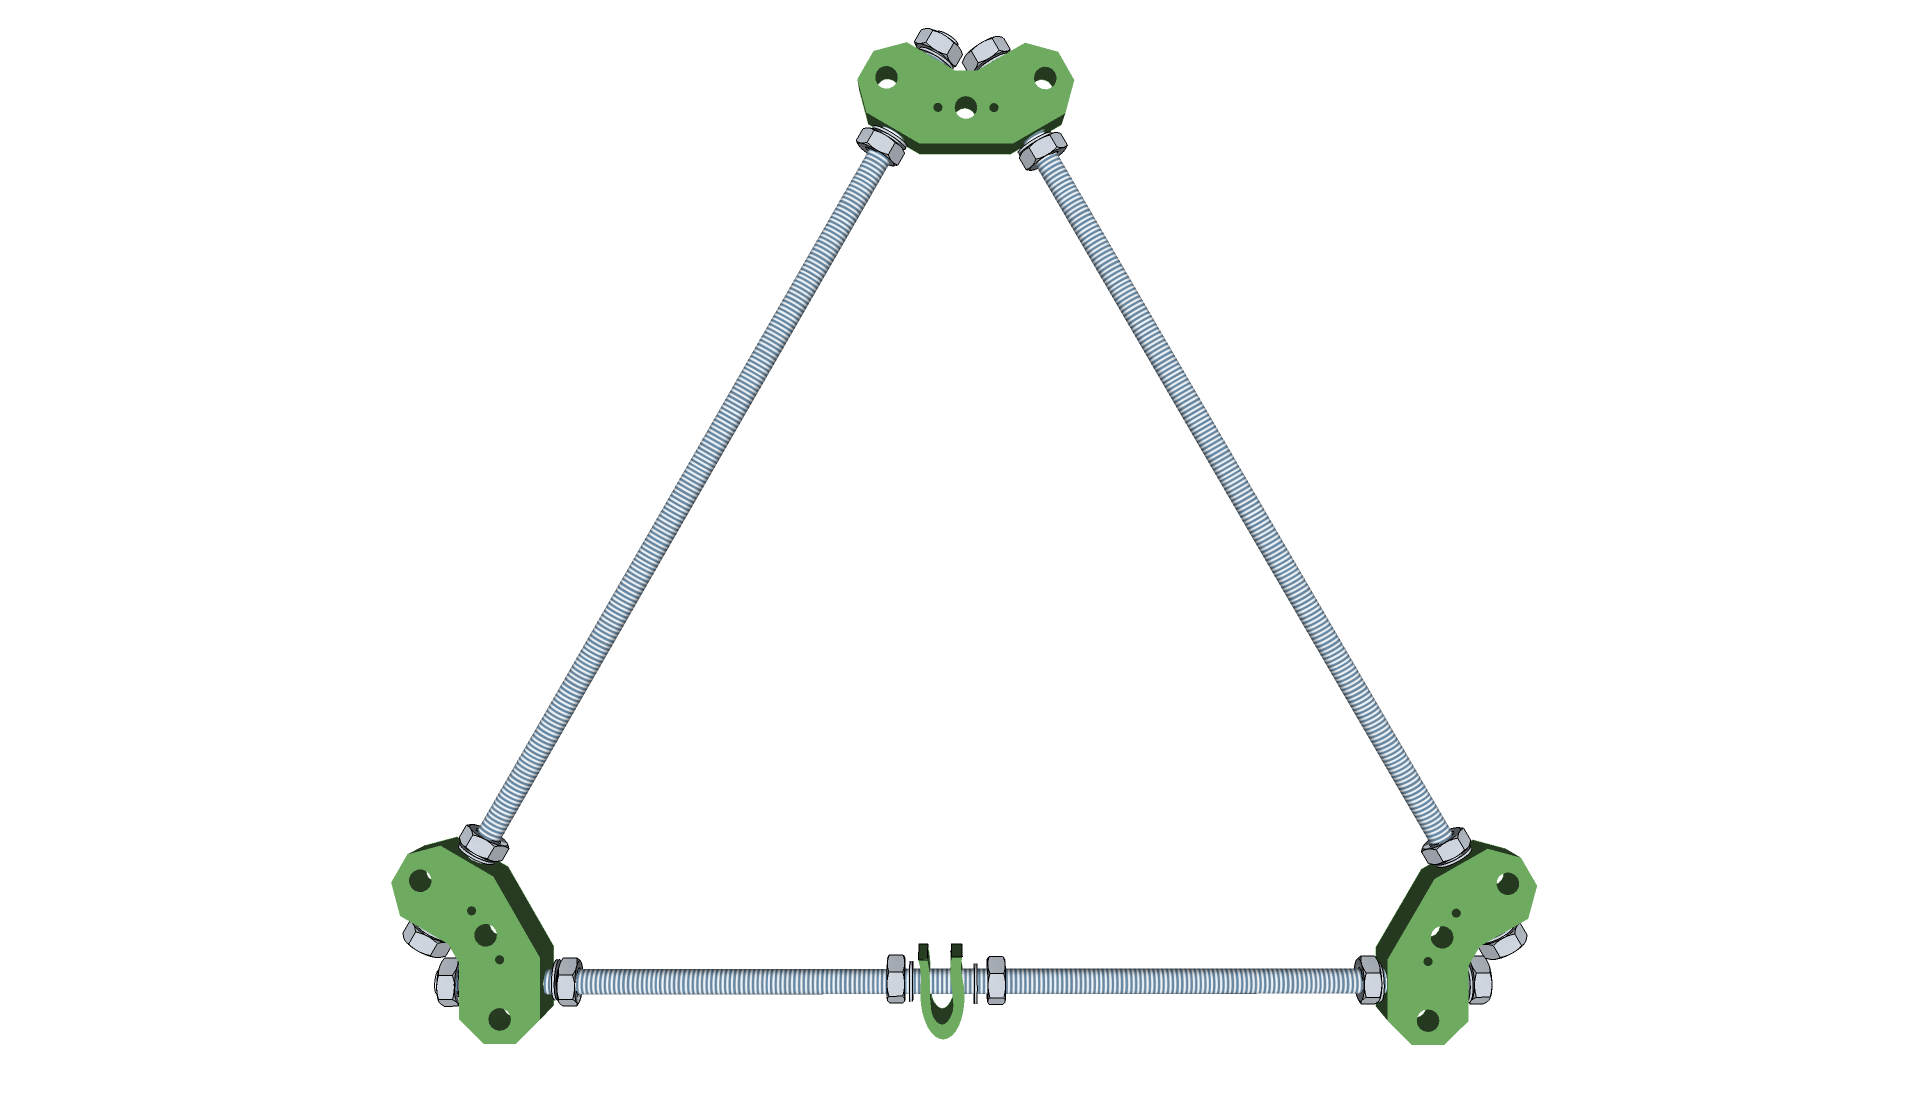
\includegraphics[width=1\linewidth]{graphics/ch1_13.png}
	
	\section{}
	That's it, that's one of the triangles done. Repeat the entire procedure for the second triangle. It is
	exactly identical to the first. \\
	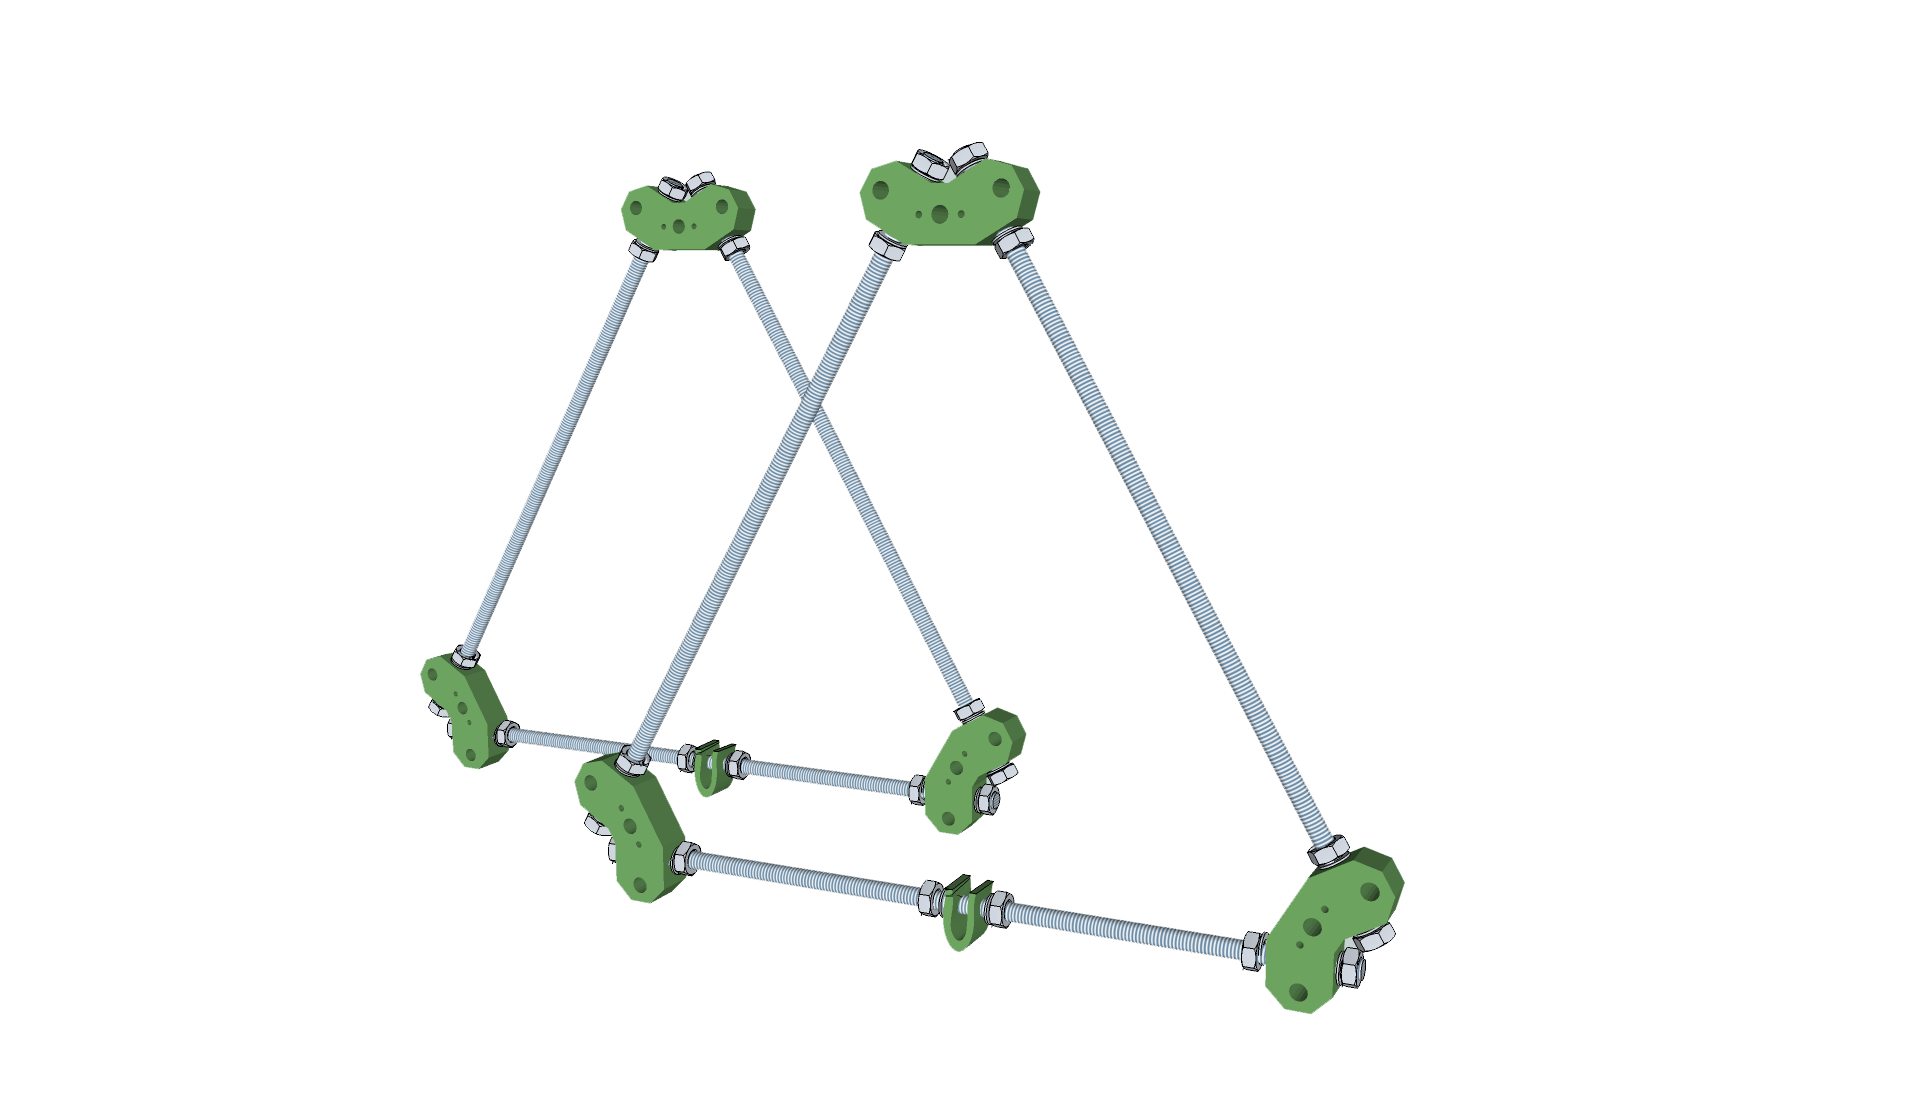
\includegraphics[width=1\linewidth]{graphics/ch1_14.png}


	
	\chapter{Assembling the front threaded rods}
	\section{}
	Thread the bottom rod first. Thread an M8 nut onto the middle of the rod. Slide an M8 washer next to it.\\
	\begin{center}
		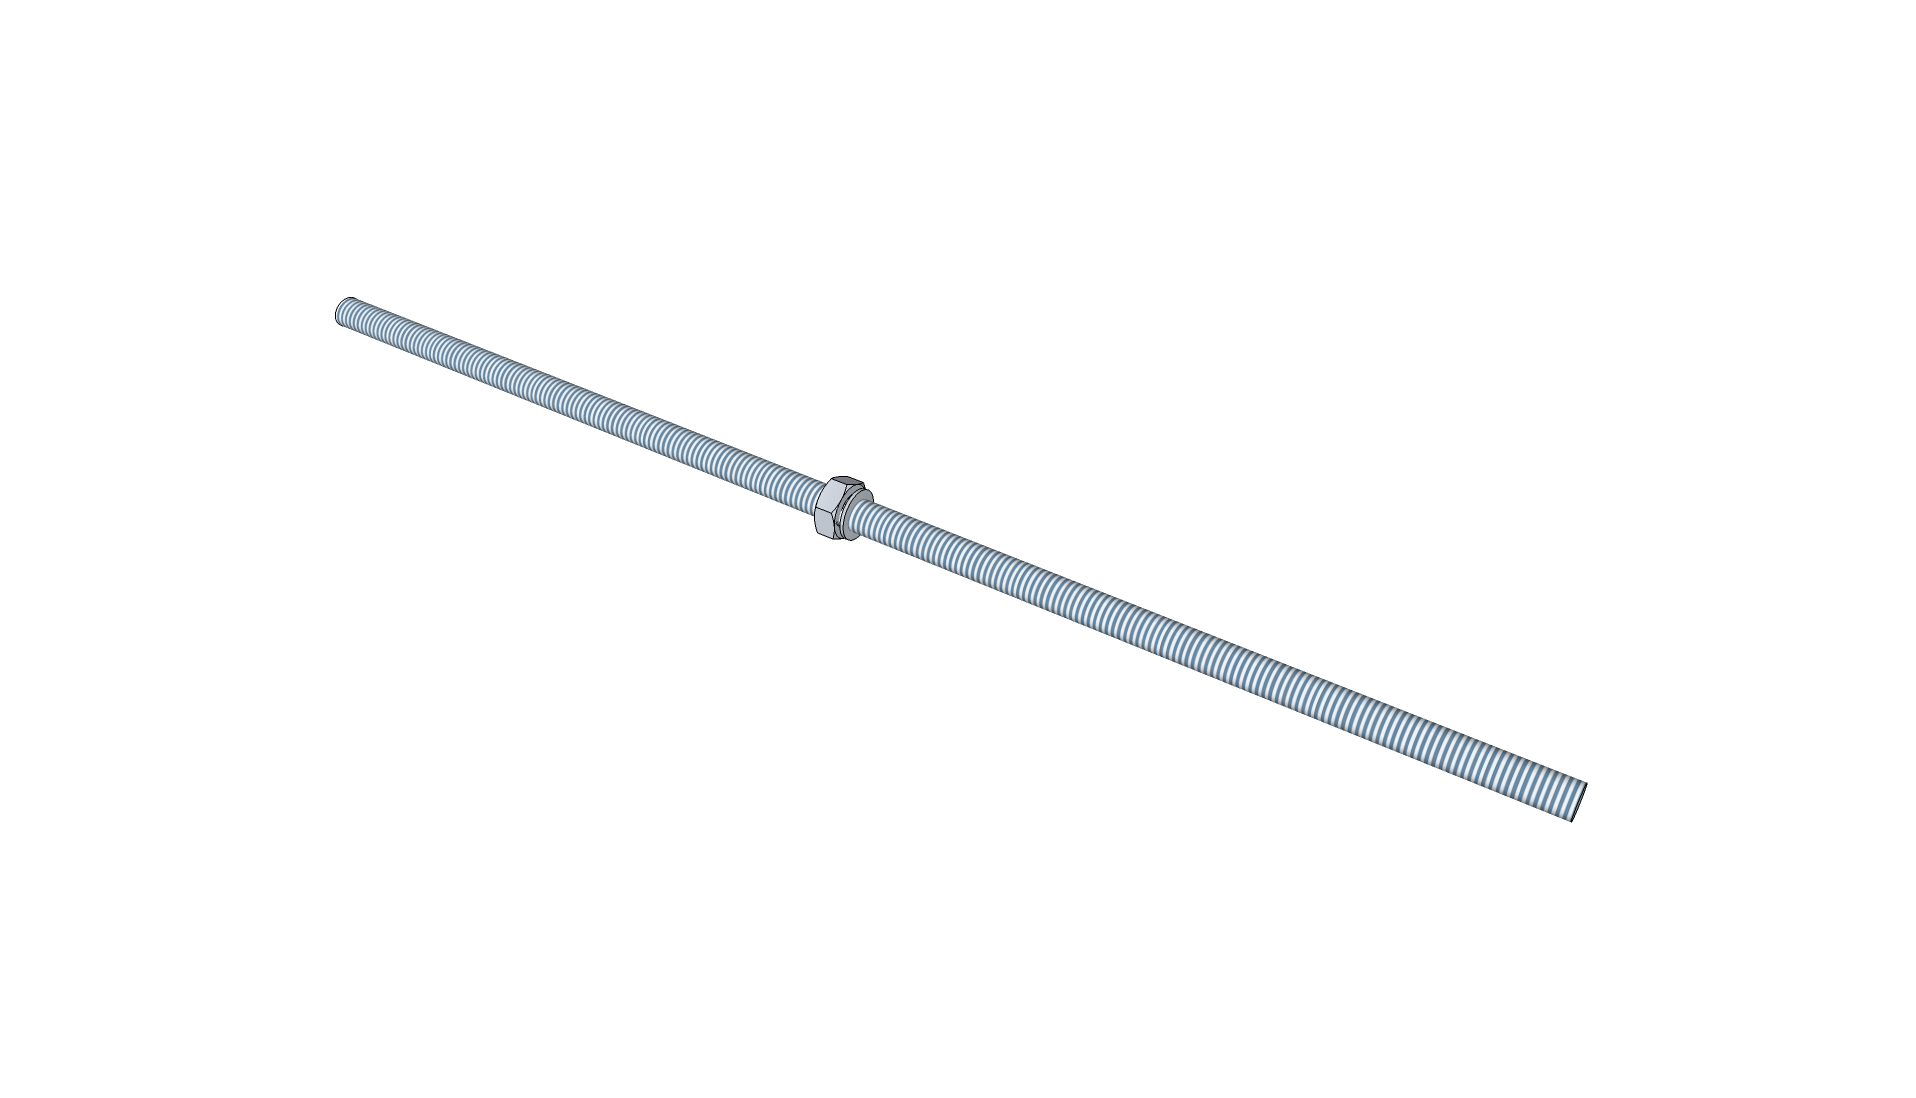
\includegraphics[width=1\linewidth]{graphics/ch2_1.png}
	\end{center}
	
	\section{}
	Thread the rod through the bottom hole of the RP y-motor-bracket. The bottom hole of the bracket is the
	long, straight side.\\
	\begin{center}
		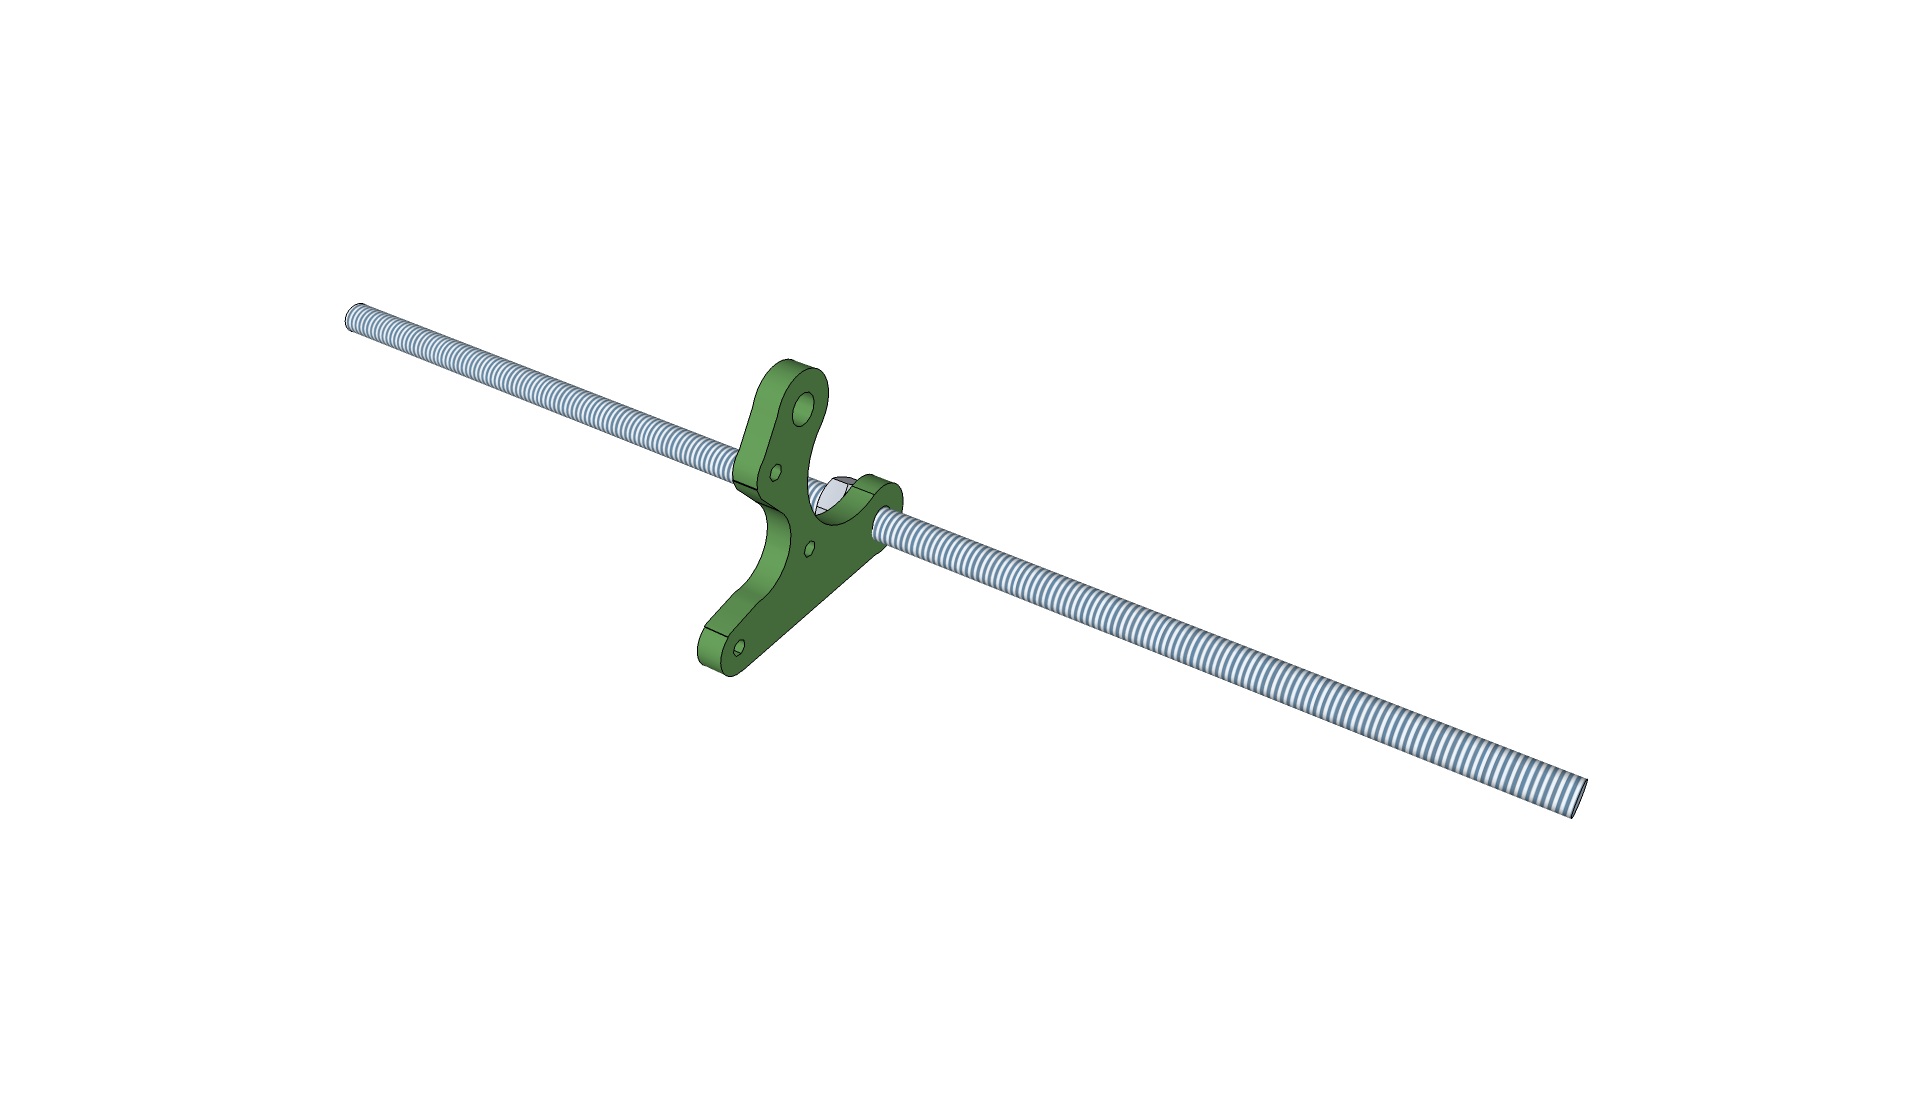
\includegraphics[width=1\linewidth]{graphics/ch2_2.png}
	\end{center}
	
	\section{}
	Slide another washer onto the other side of the rod and add another M8 nut to hold it in place.\\
	\begin{center}
		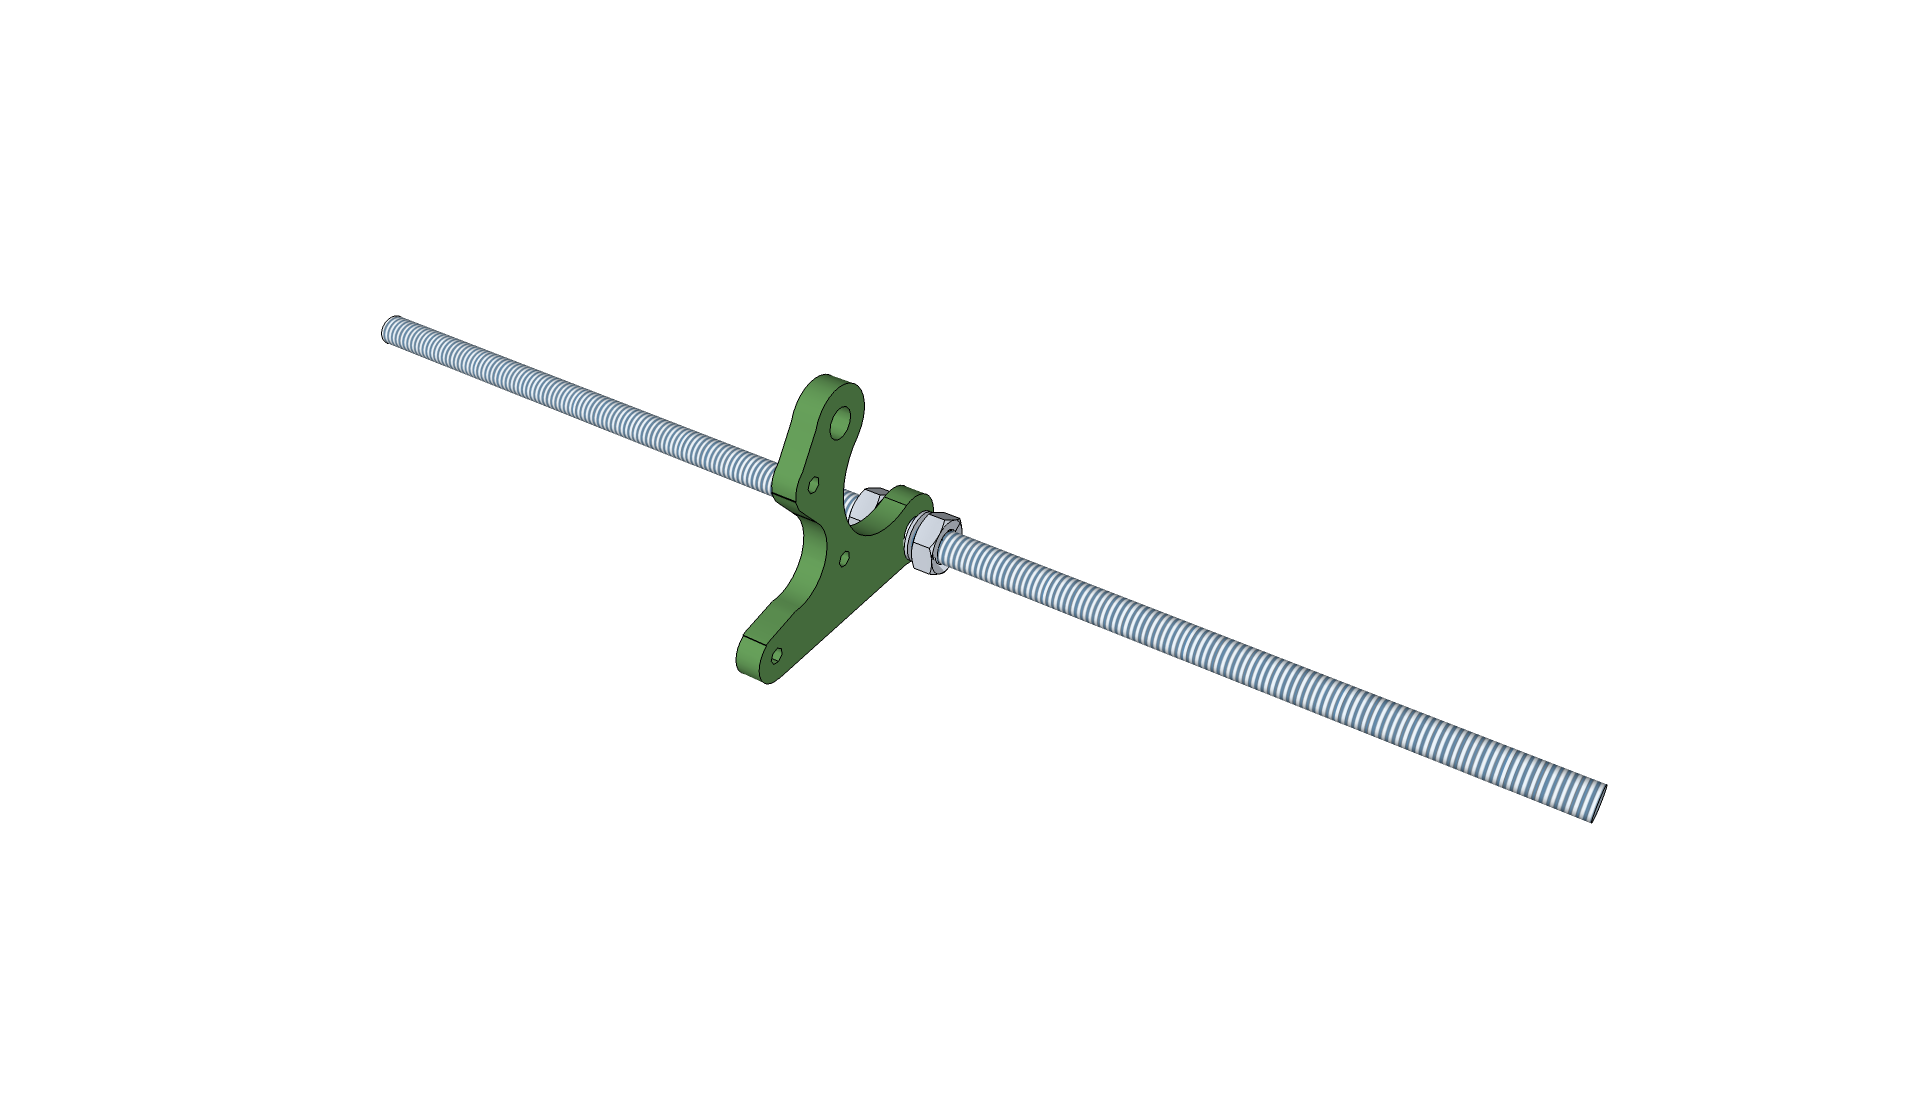
\includegraphics[width=1\linewidth]{graphics/ch2_3.png}
	\end{center}
	
	\section{}
	Add a nut and washer to each end of the rod.\\
	\begin{center}
		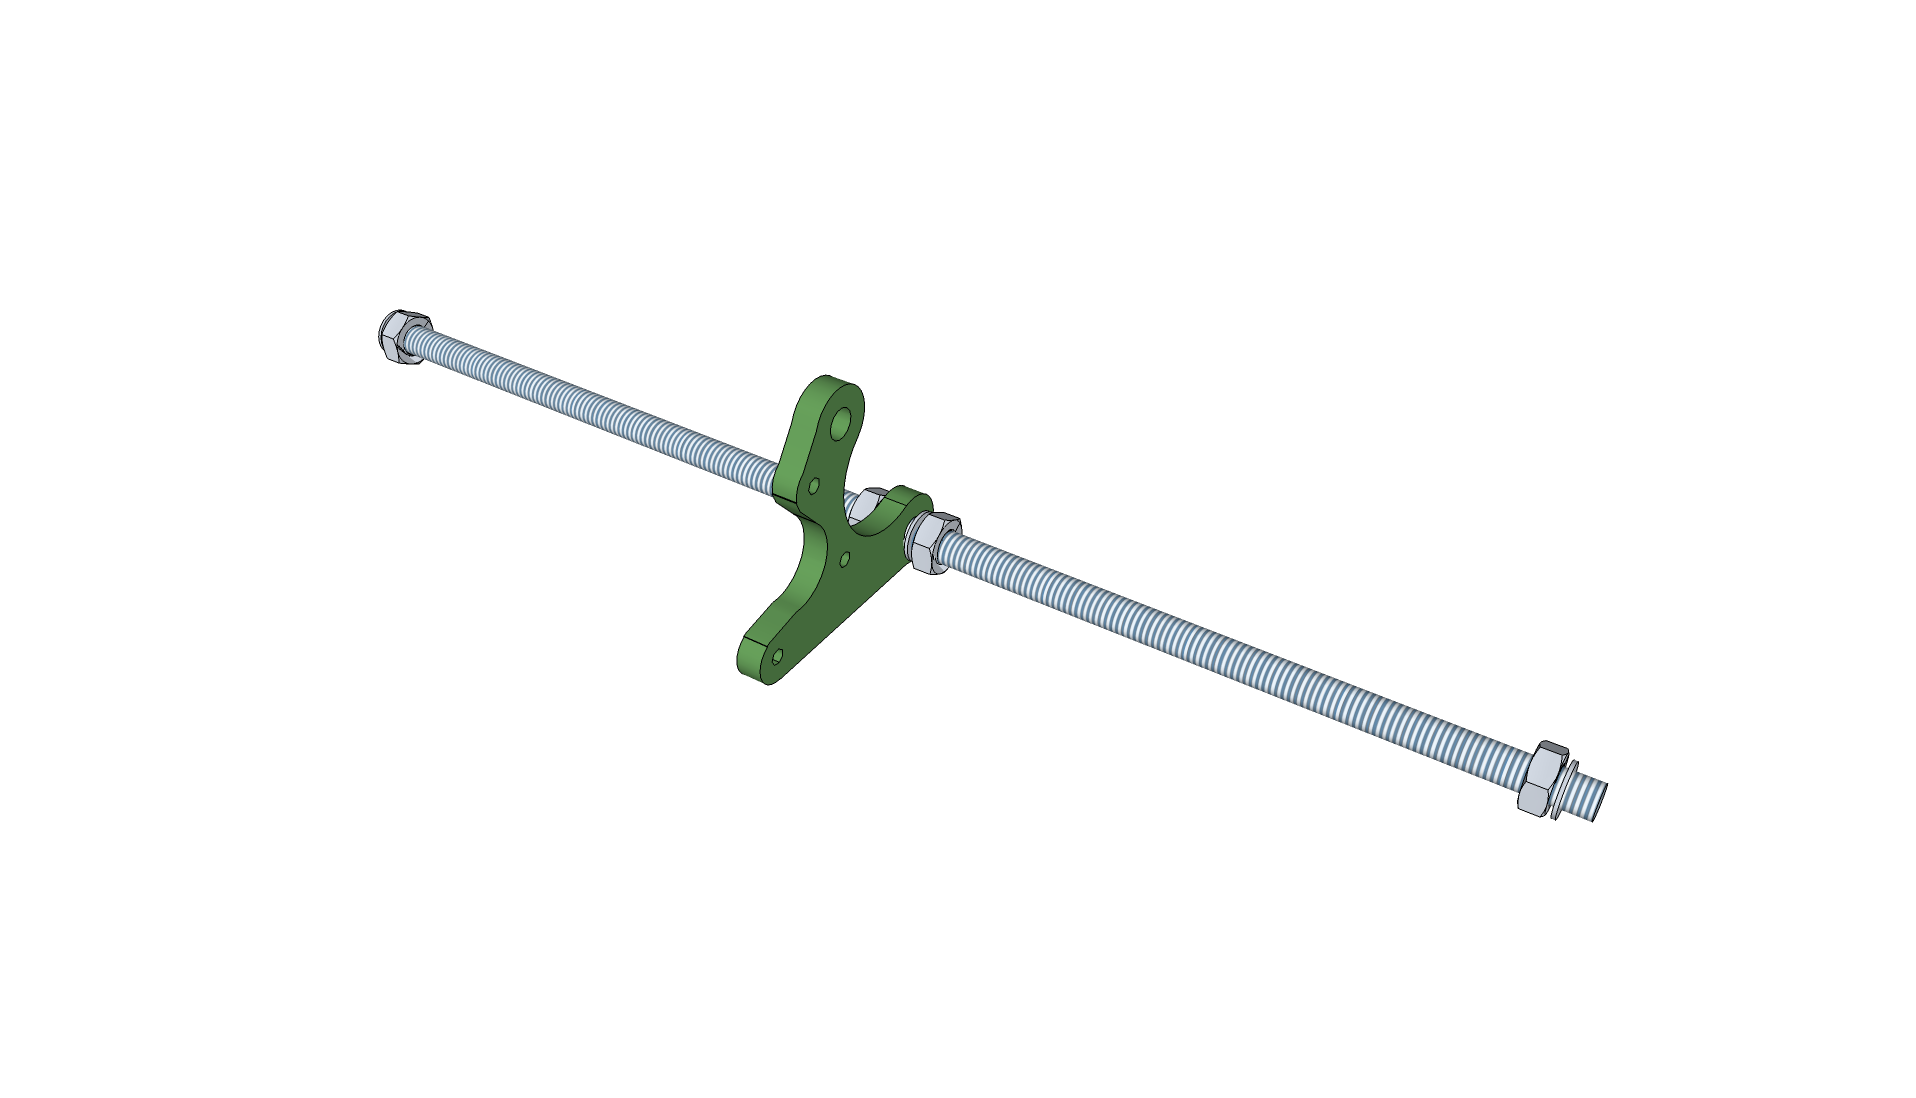
\includegraphics[width=1\linewidth]{graphics/ch2_4.png}
	\end{center}
	
	\section{}
	Now thread the top rod. This is a complicated one, so make sure you get it all done in the right order.
	From left to right, the rod should have: 1 washer, 2 nuts, 1 washer, 1 bar clamp (threaded through the
	holes), 1 washer, 2 nuts, 1 washer, the y-motor-bracket (with the pointy bit pointed towards you),1
	washer, 1 nut, 2 washers, 1 fender/mudguard washer, 1 washer, 1 608 bearing, 1 washer,1 fender/
	mudguard washer, 2 nuts, 1 washer, 1 bar clamp (threaded through the holes), 1 washer, 2 nuts, 1
	washer.\\
	\begin{center}
		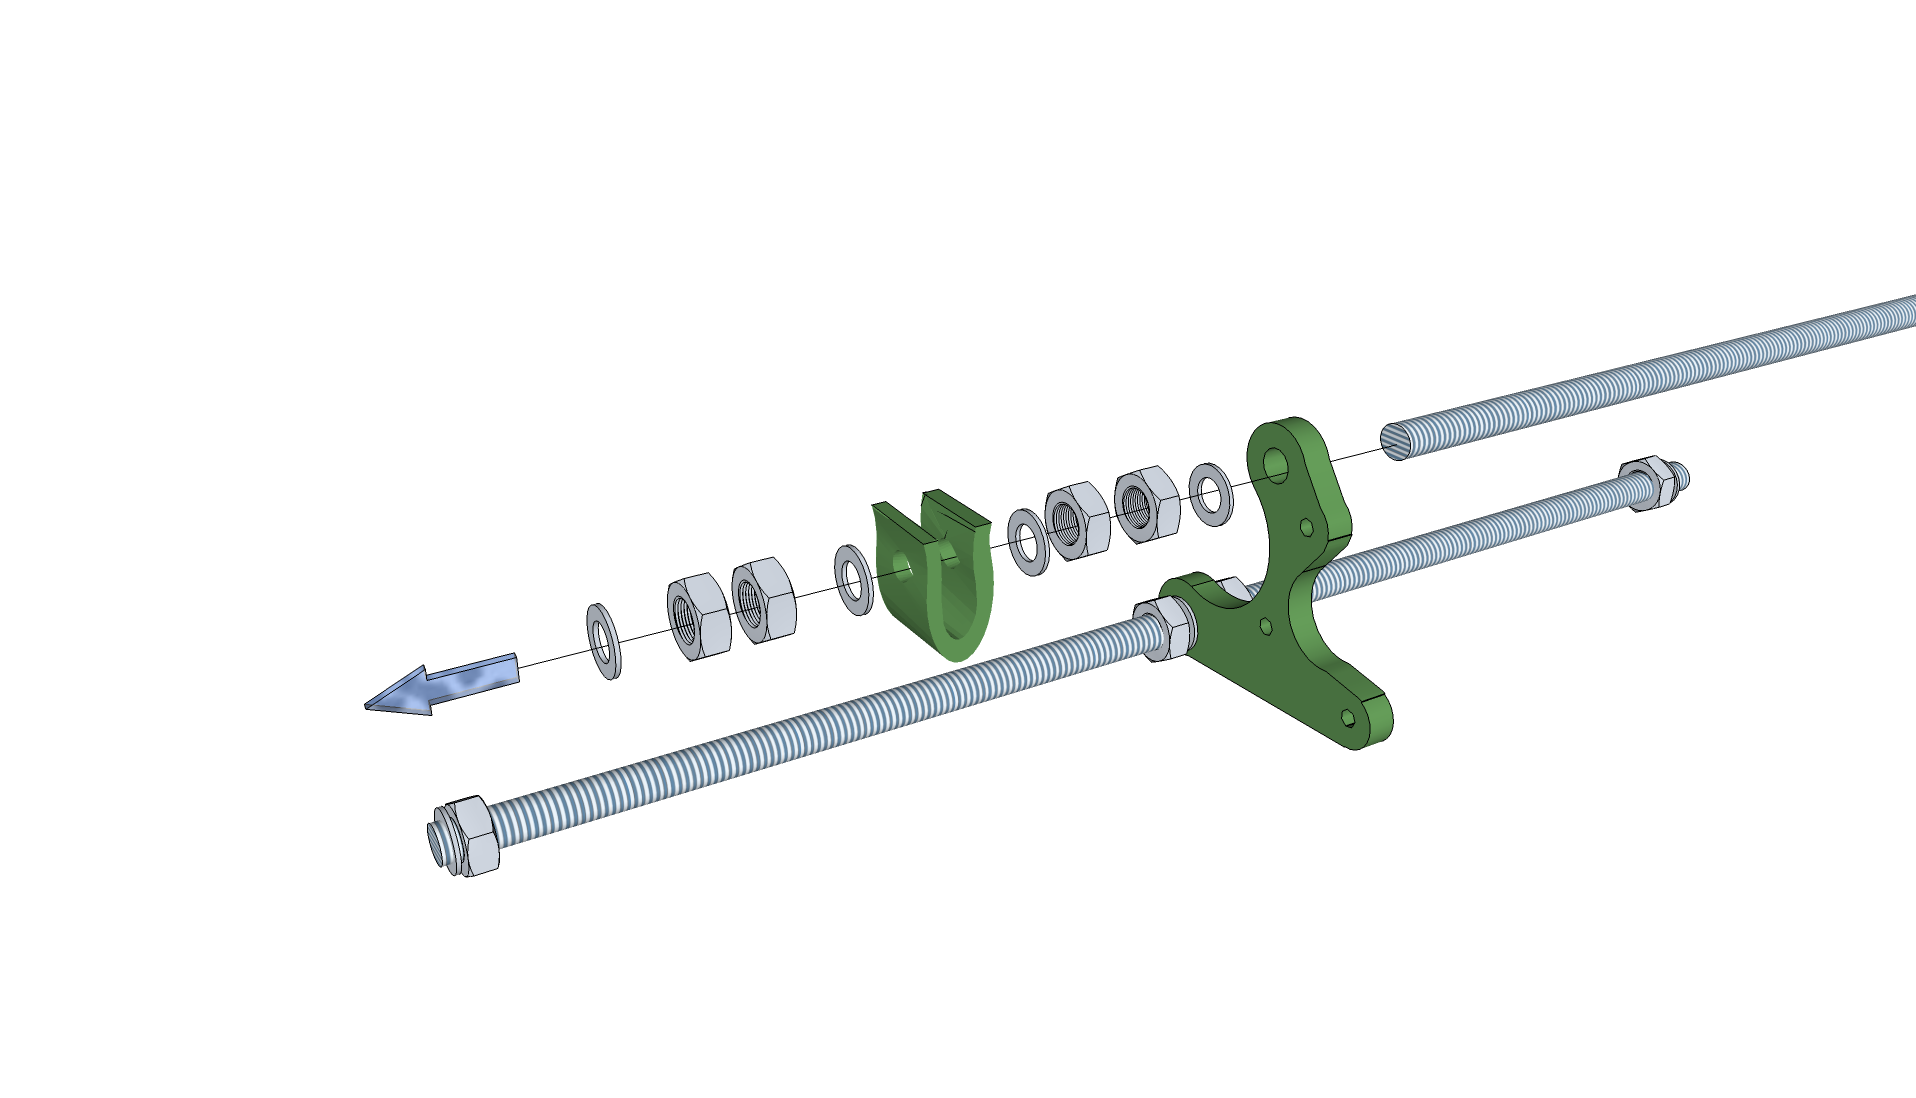
\includegraphics[width=1\linewidth]{graphics/ch2_5_1.png}
	\end{center}
	[ Lefthand Side ]
	\begin{center}
		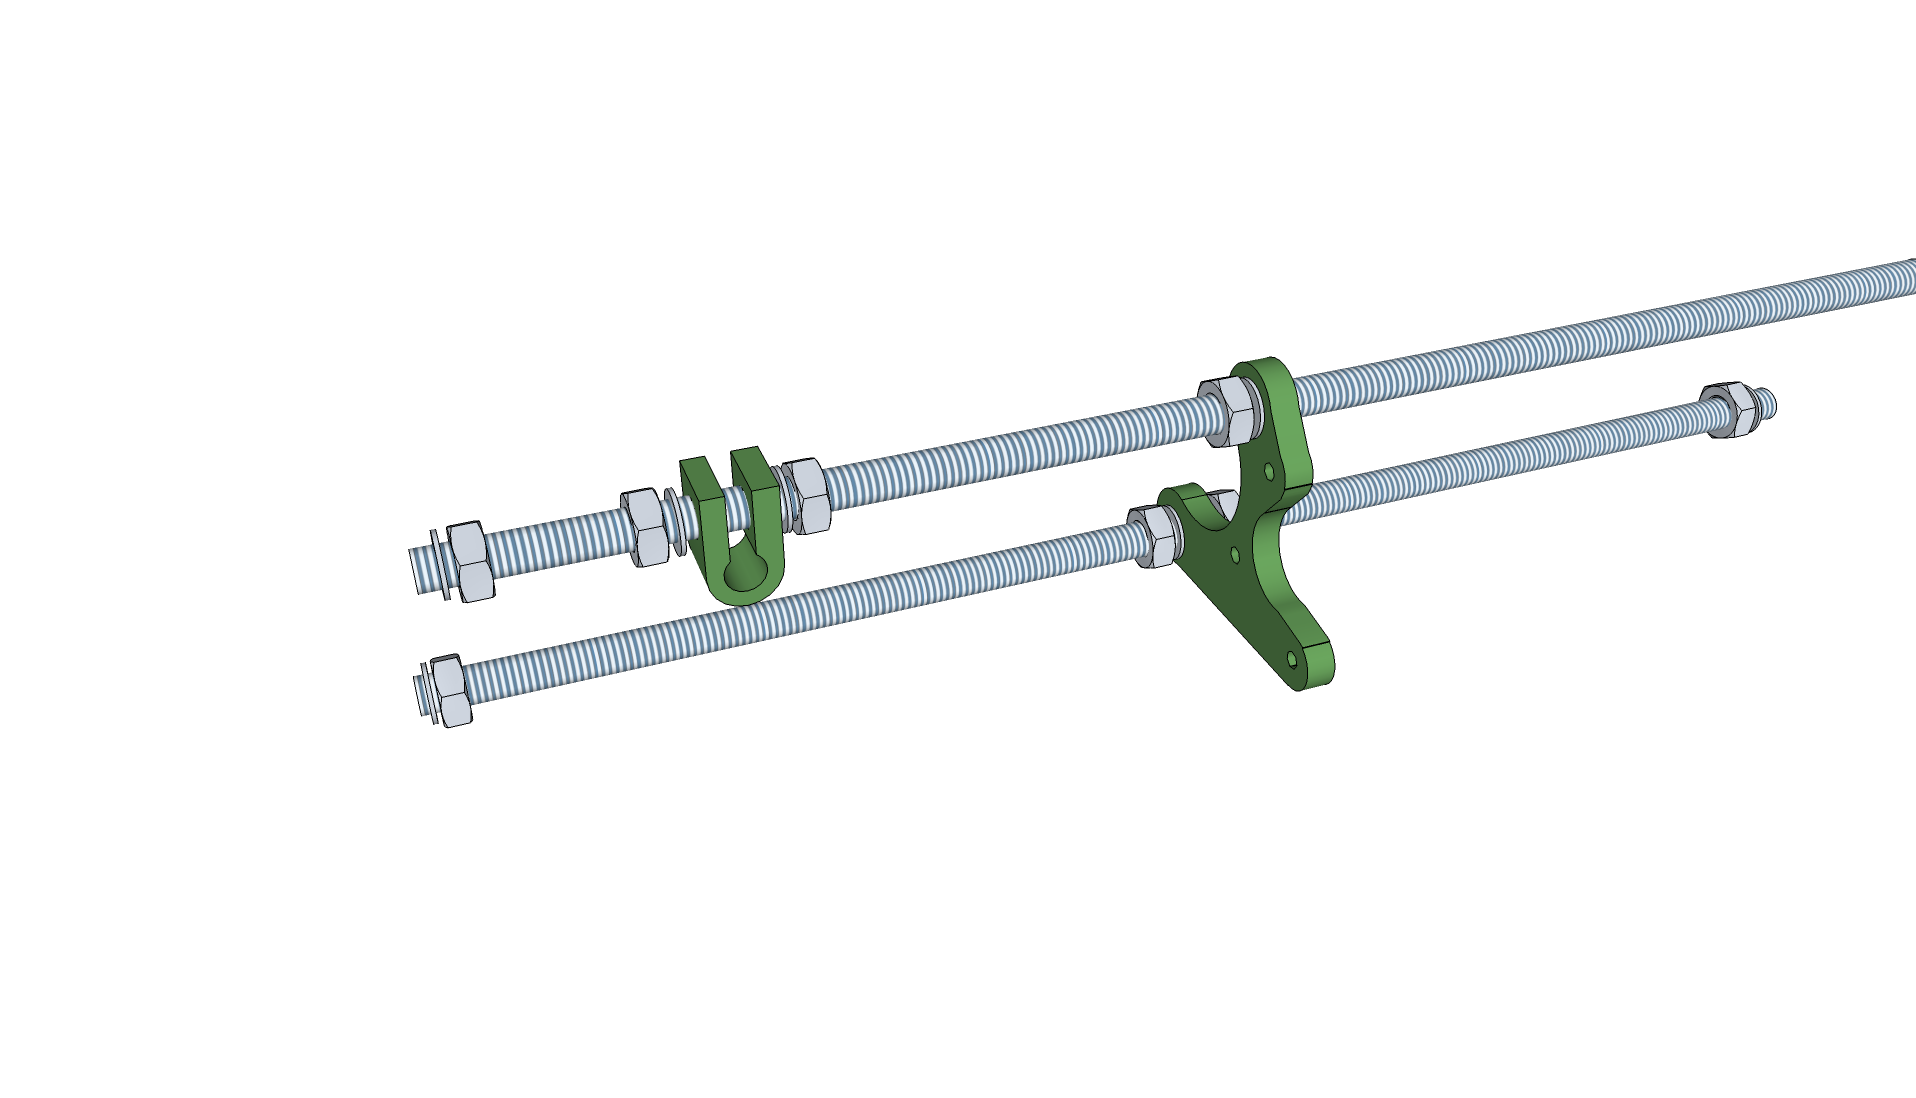
\includegraphics[width=1\linewidth]{graphics/ch2_5_2.png}
	\end{center}
	\begin{overpic}[width=1\linewidth]{graphics/ch2_5_3.png}
		\put(0,0){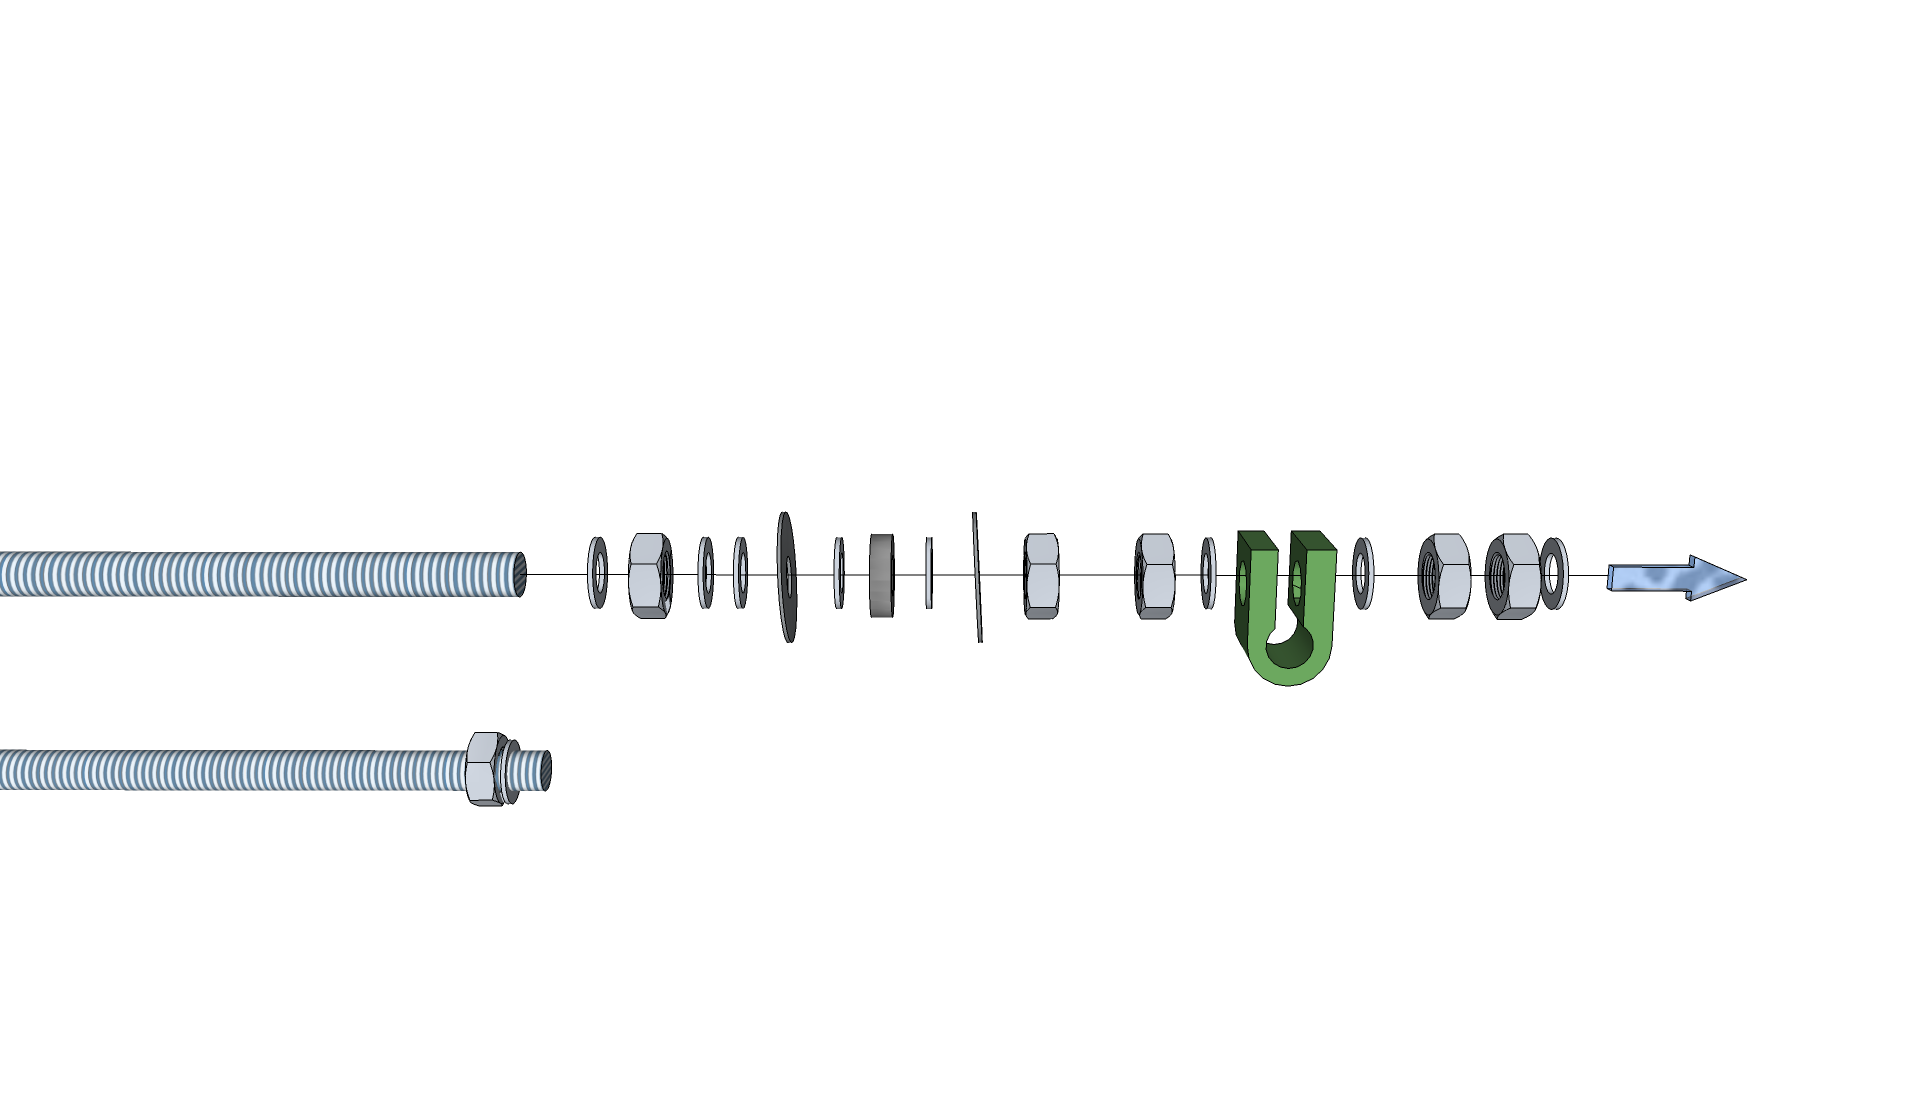
\includegraphics[width=0.4\linewidth]{graphics/ch2_5_4.png}}
	\end{overpic}
	[ Righthand Side ]
	\begin{center}
		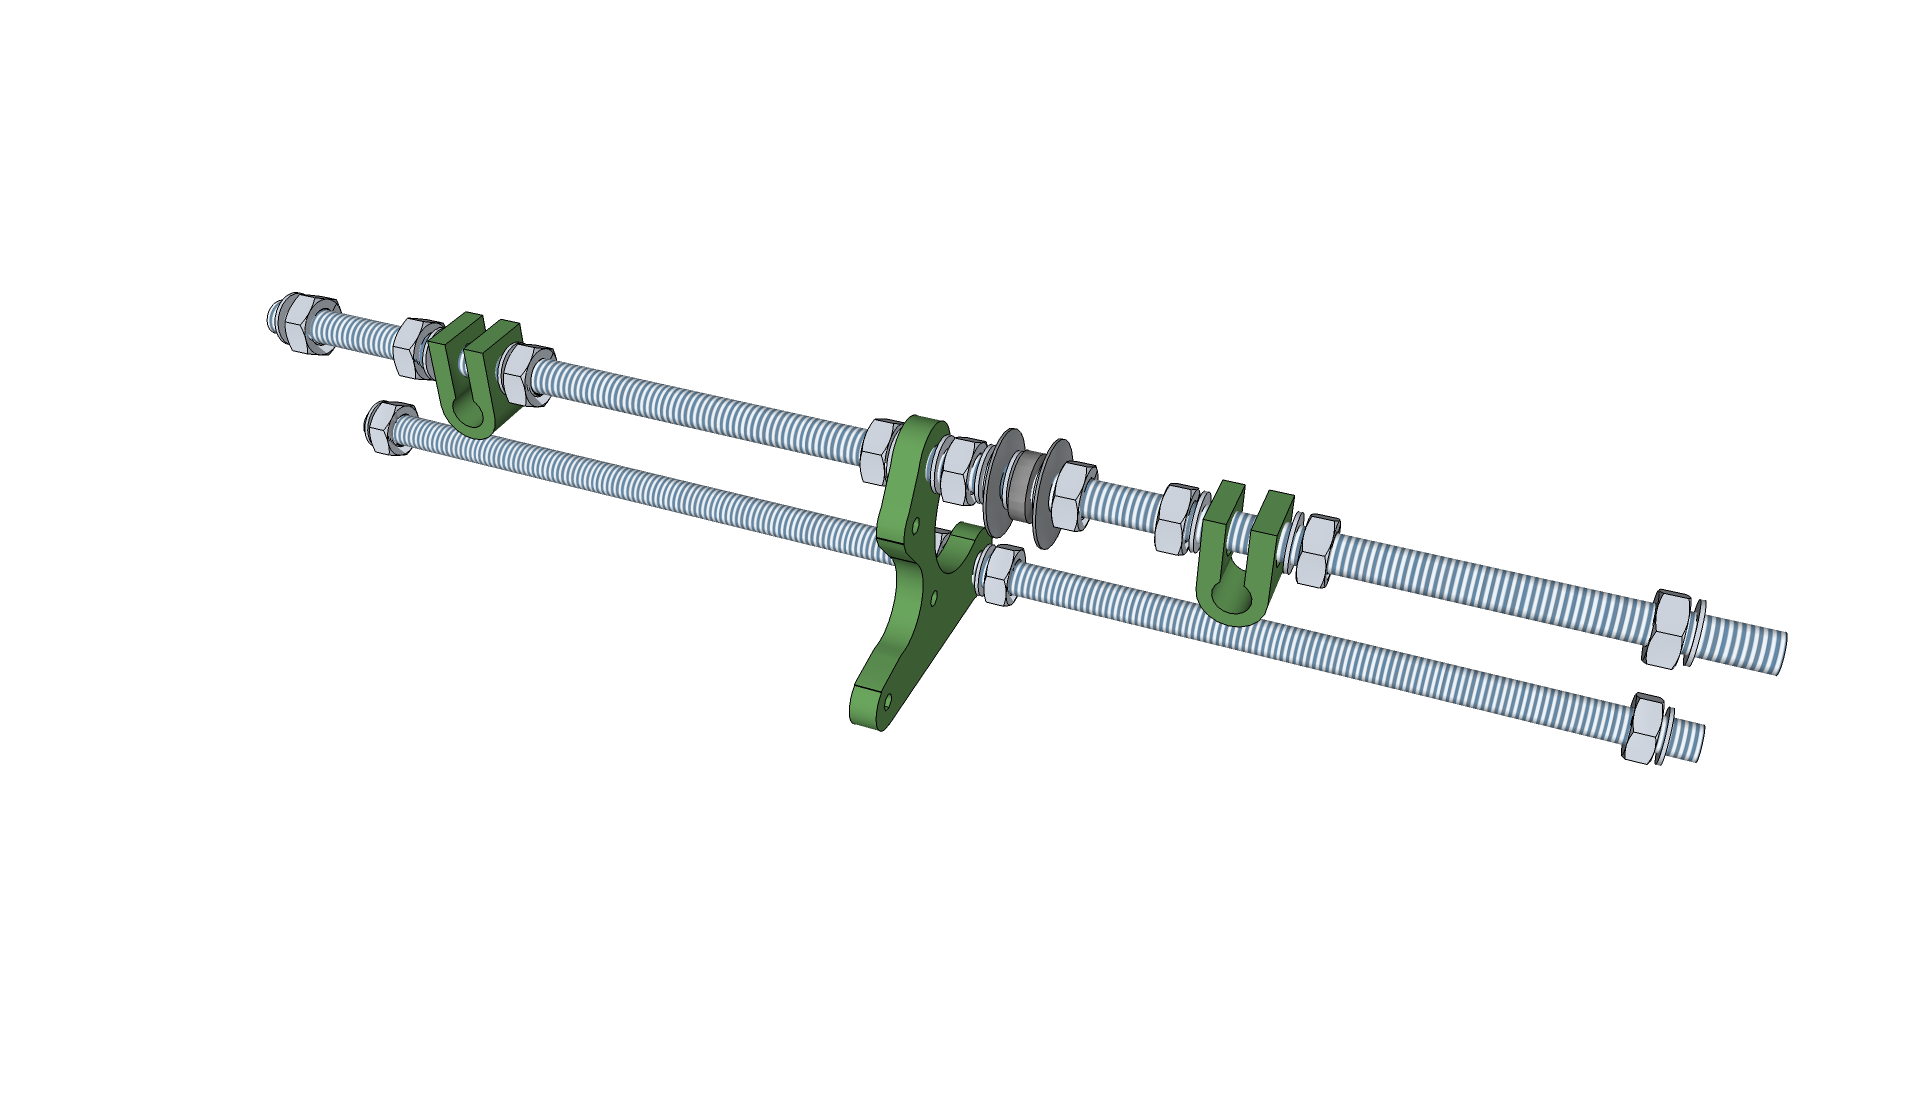
\includegraphics[width=1\linewidth]{graphics/ch2_5_5.png}
	\end{center}
	
	\section{}
	When you hold it with the bigger part (with the circular hole) of the motor bracket towards you, it should
	look like the picture below. Verify this now.\\
	\begin{center}
		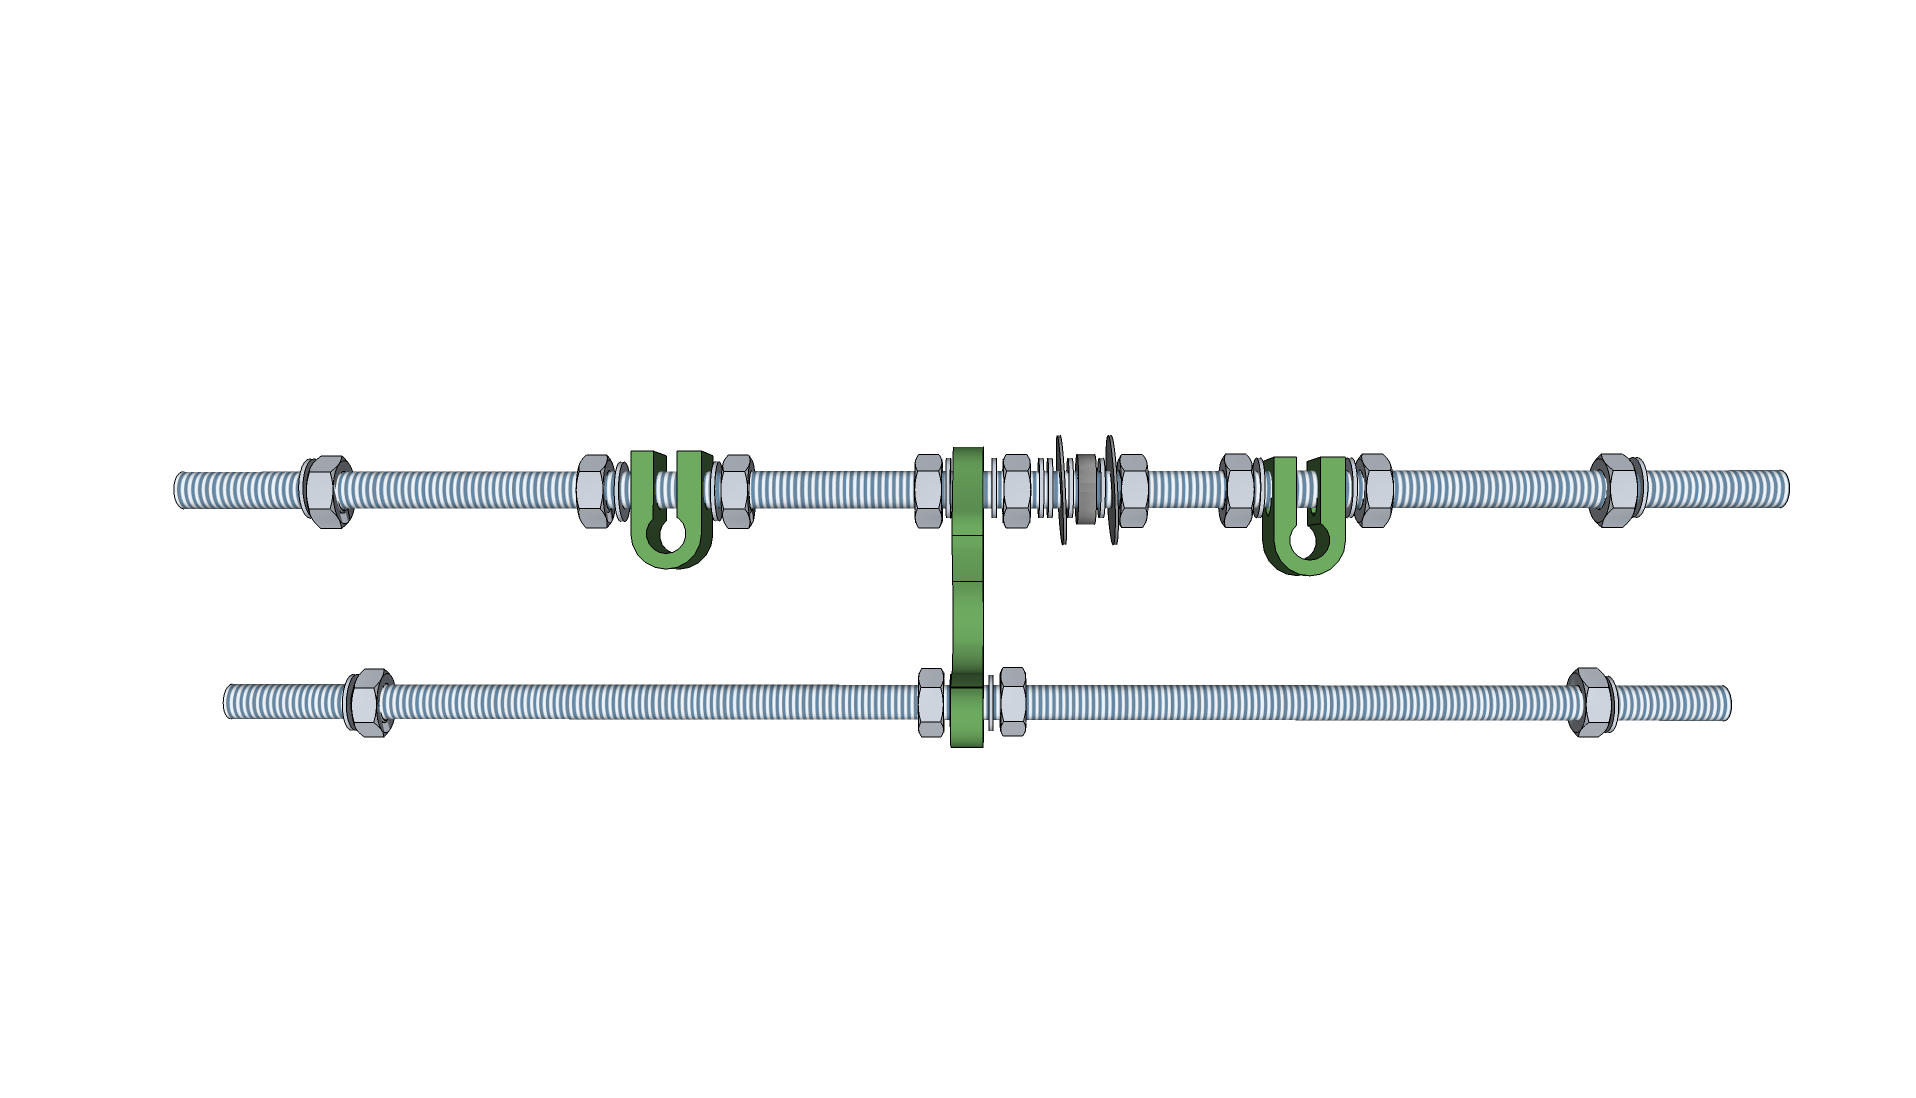
\includegraphics[width=1\linewidth]{graphics/ch2_6.png}
	\end{center}
	
	\section{}
	You can now attach this setup to the triangle sides. Make sure the bigger part of the motor bracket
	points OUT of the triangle. Thread the ends of the rods through two of the footed vertices. Put a washer
	and nut on the end of each threaded rod. It should now look like this:
	\begin{center}
		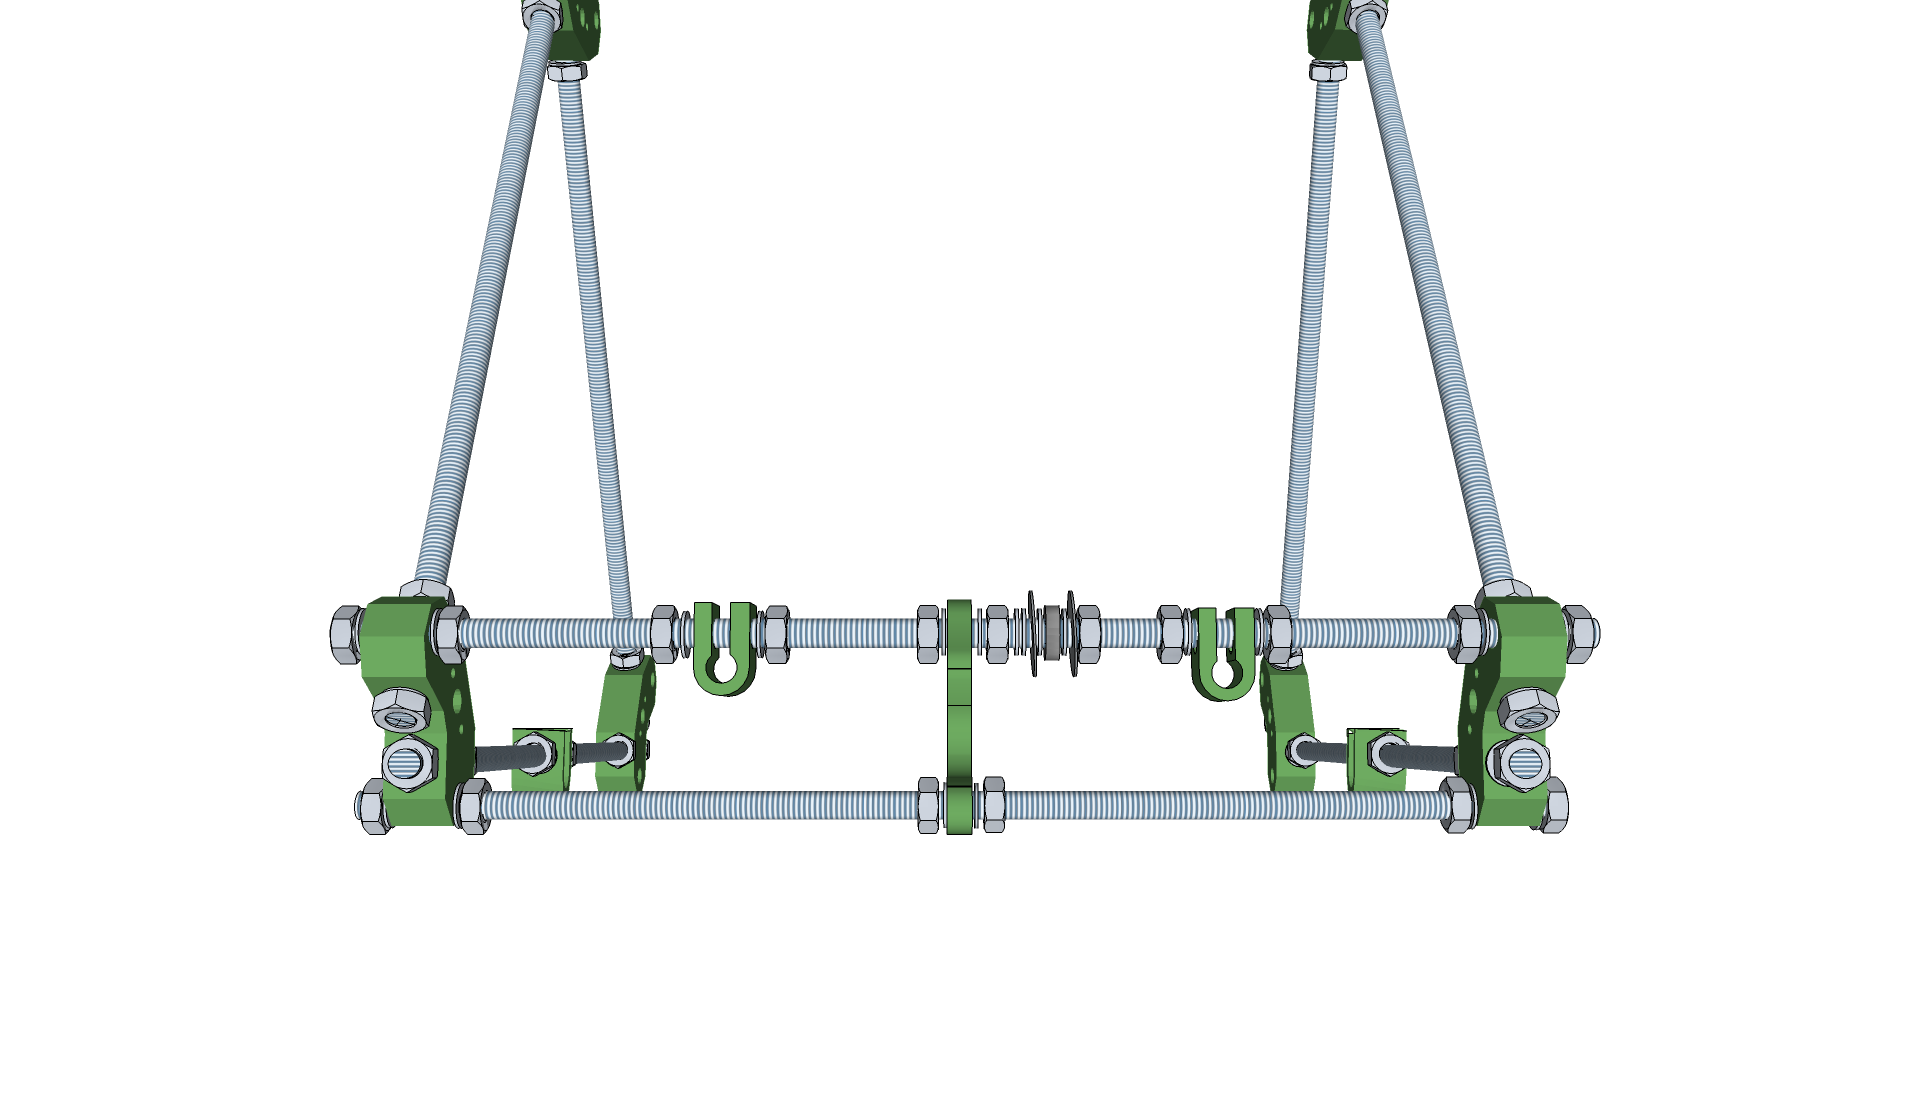
\includegraphics[width=1\linewidth]{graphics/ch2_7_1.png}
	\end{center}
	\begin{center}
		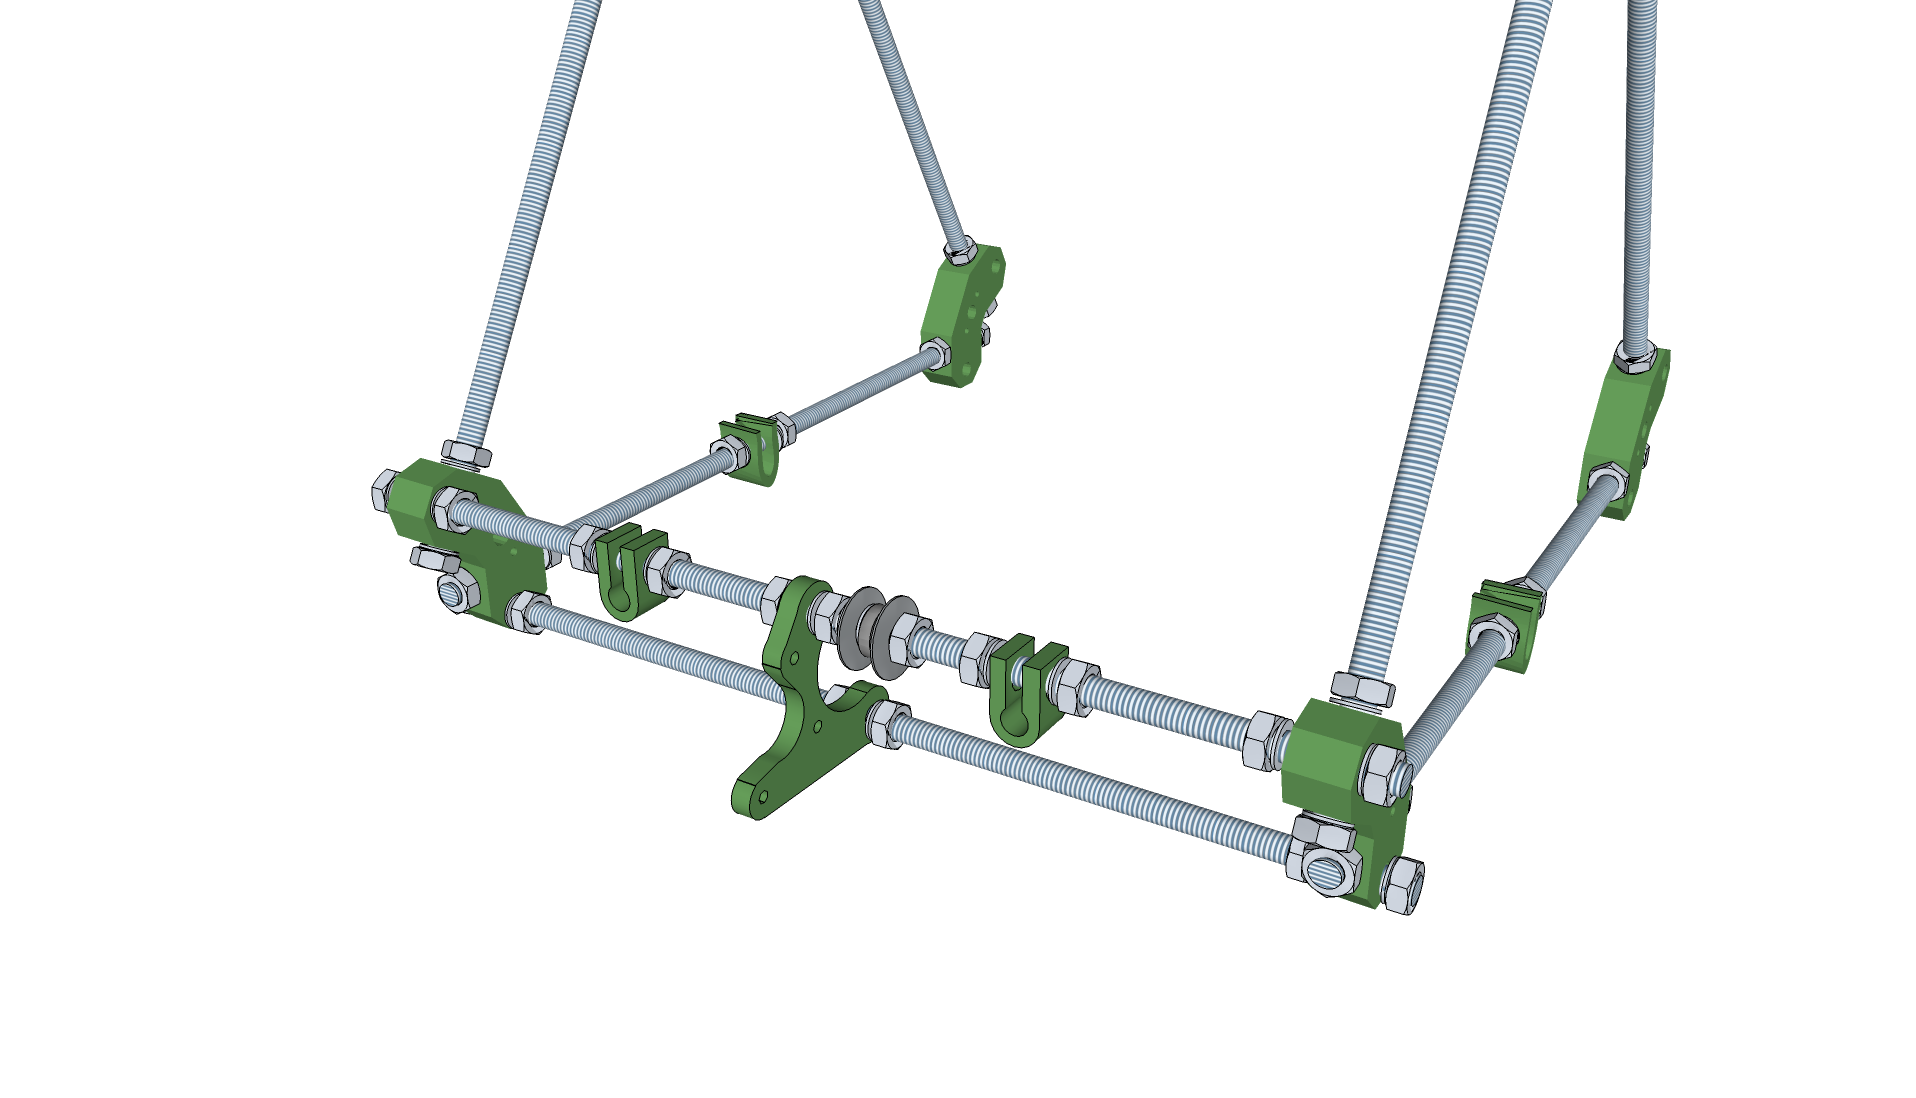
\includegraphics[width=1\linewidth]{graphics/ch2_7_2.png}
	\end{center}
	\begin{center}
		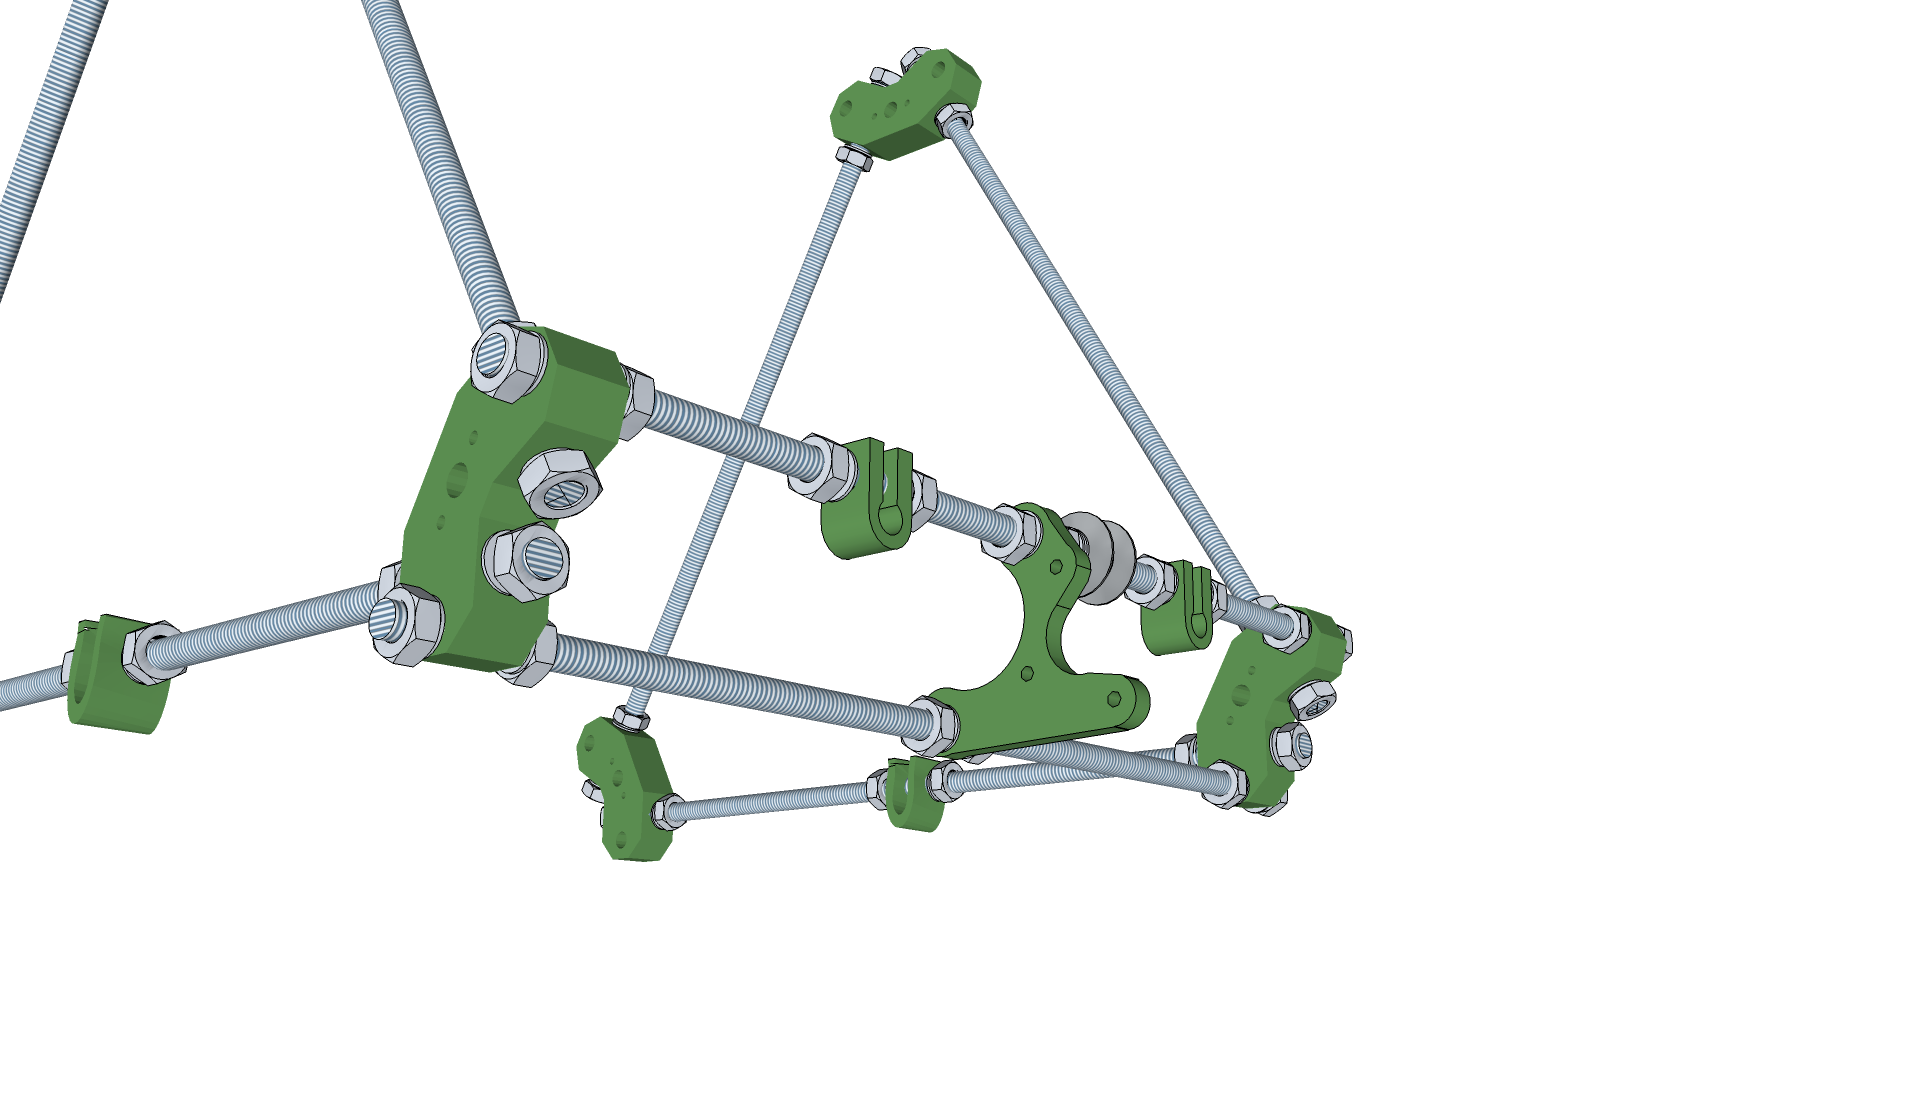
\includegraphics[width=1\linewidth]{graphics/ch2_7_3.png}
	\end{center}
	[ View from below ]
	
	\chapter{Assembling the rear threaded rods}
	
	\section{}
	Thread the bottom rod first. Add a nut and washer to each end of the rod.\\
	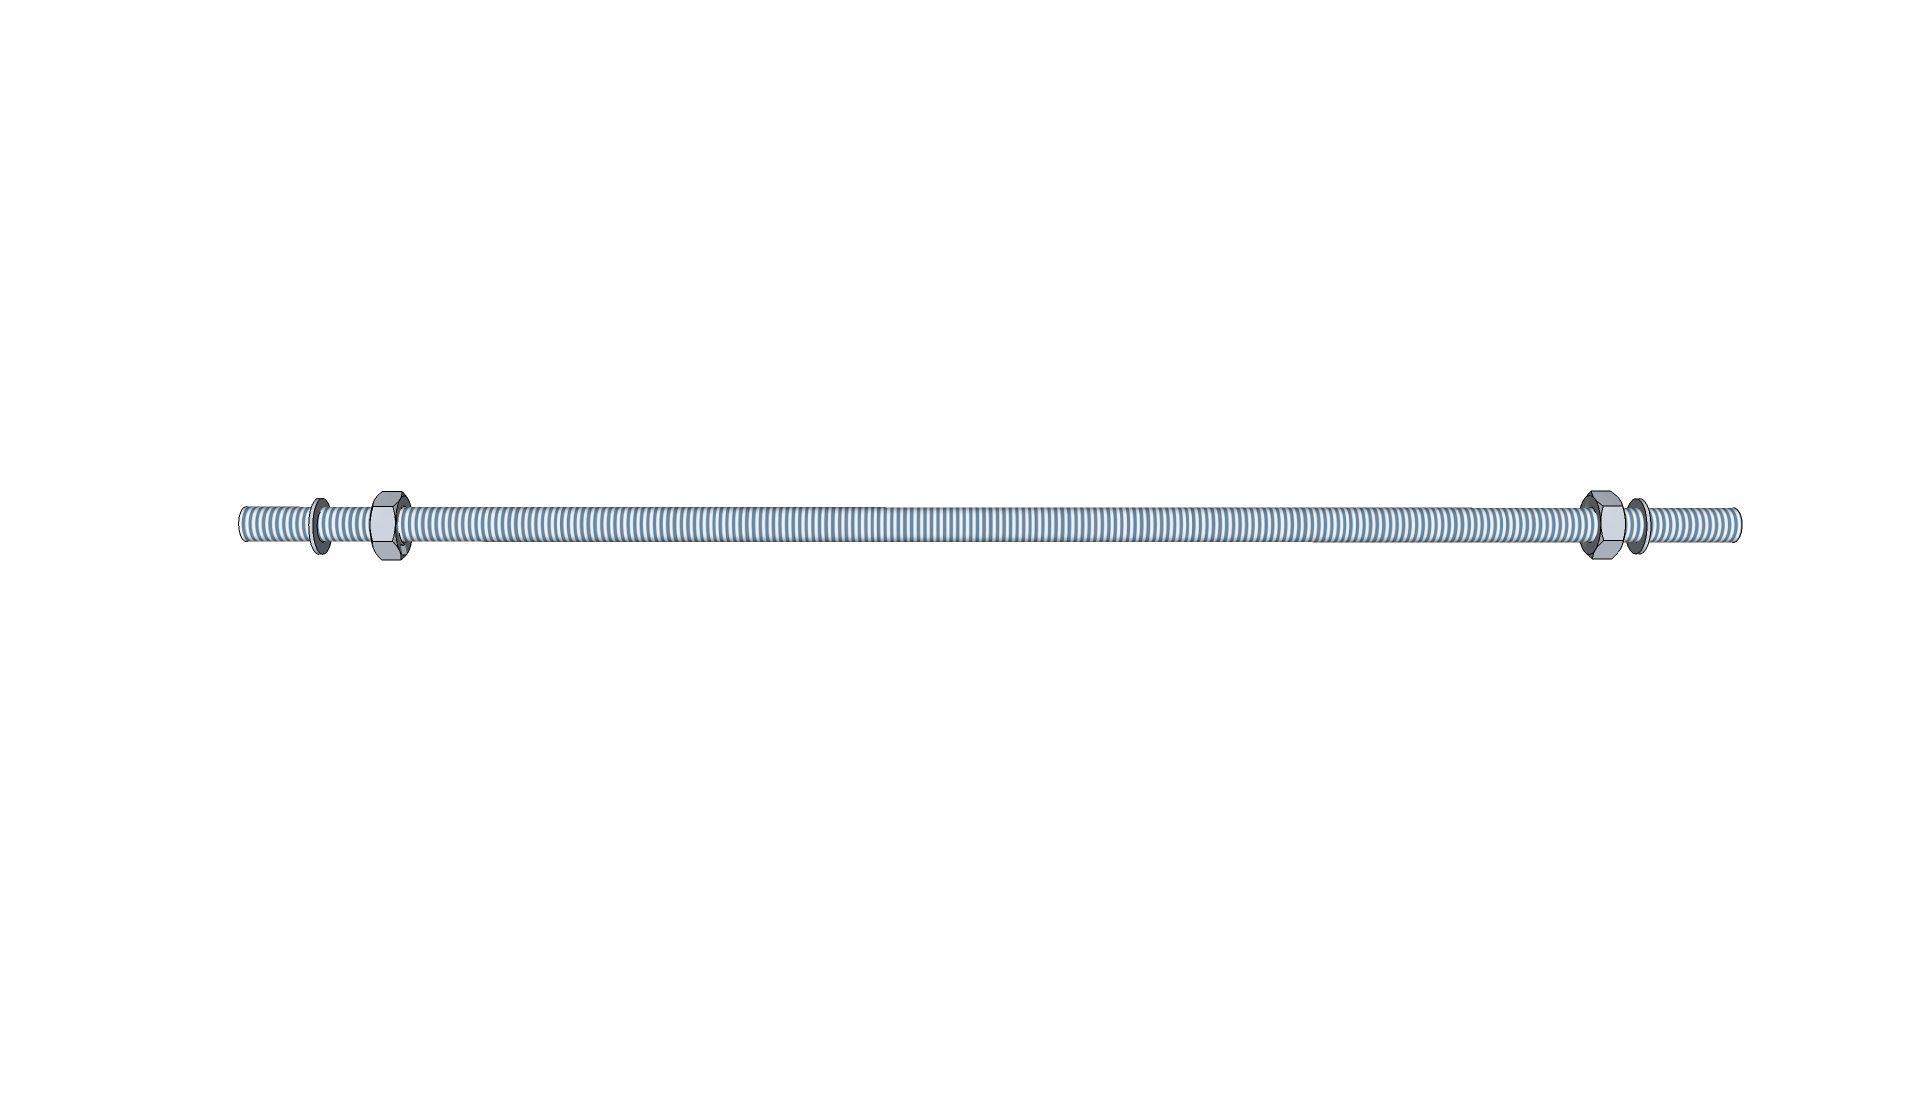
\includegraphics[width=1\linewidth]{graphics/ch3_1.png}
	
	\section{}
	Now thread the top rod. This is again a complicated one, so make sure you get it all done in the right
	order. From left to right, the rod should have: 1 washer, 2 nuts, 1 washer, 1 bar clamp (threaded
	through the holes), 1 washer, 2 nuts, 1 fender/mudguard washer, 1 washer, 1 608 bearing, 1 washer,1
	fender/mudguard washer, 2 nuts, 1 washer, 1 bar clamp (threaded through the holes), 1 washer, 2 nuts,
	1 washer.\\
	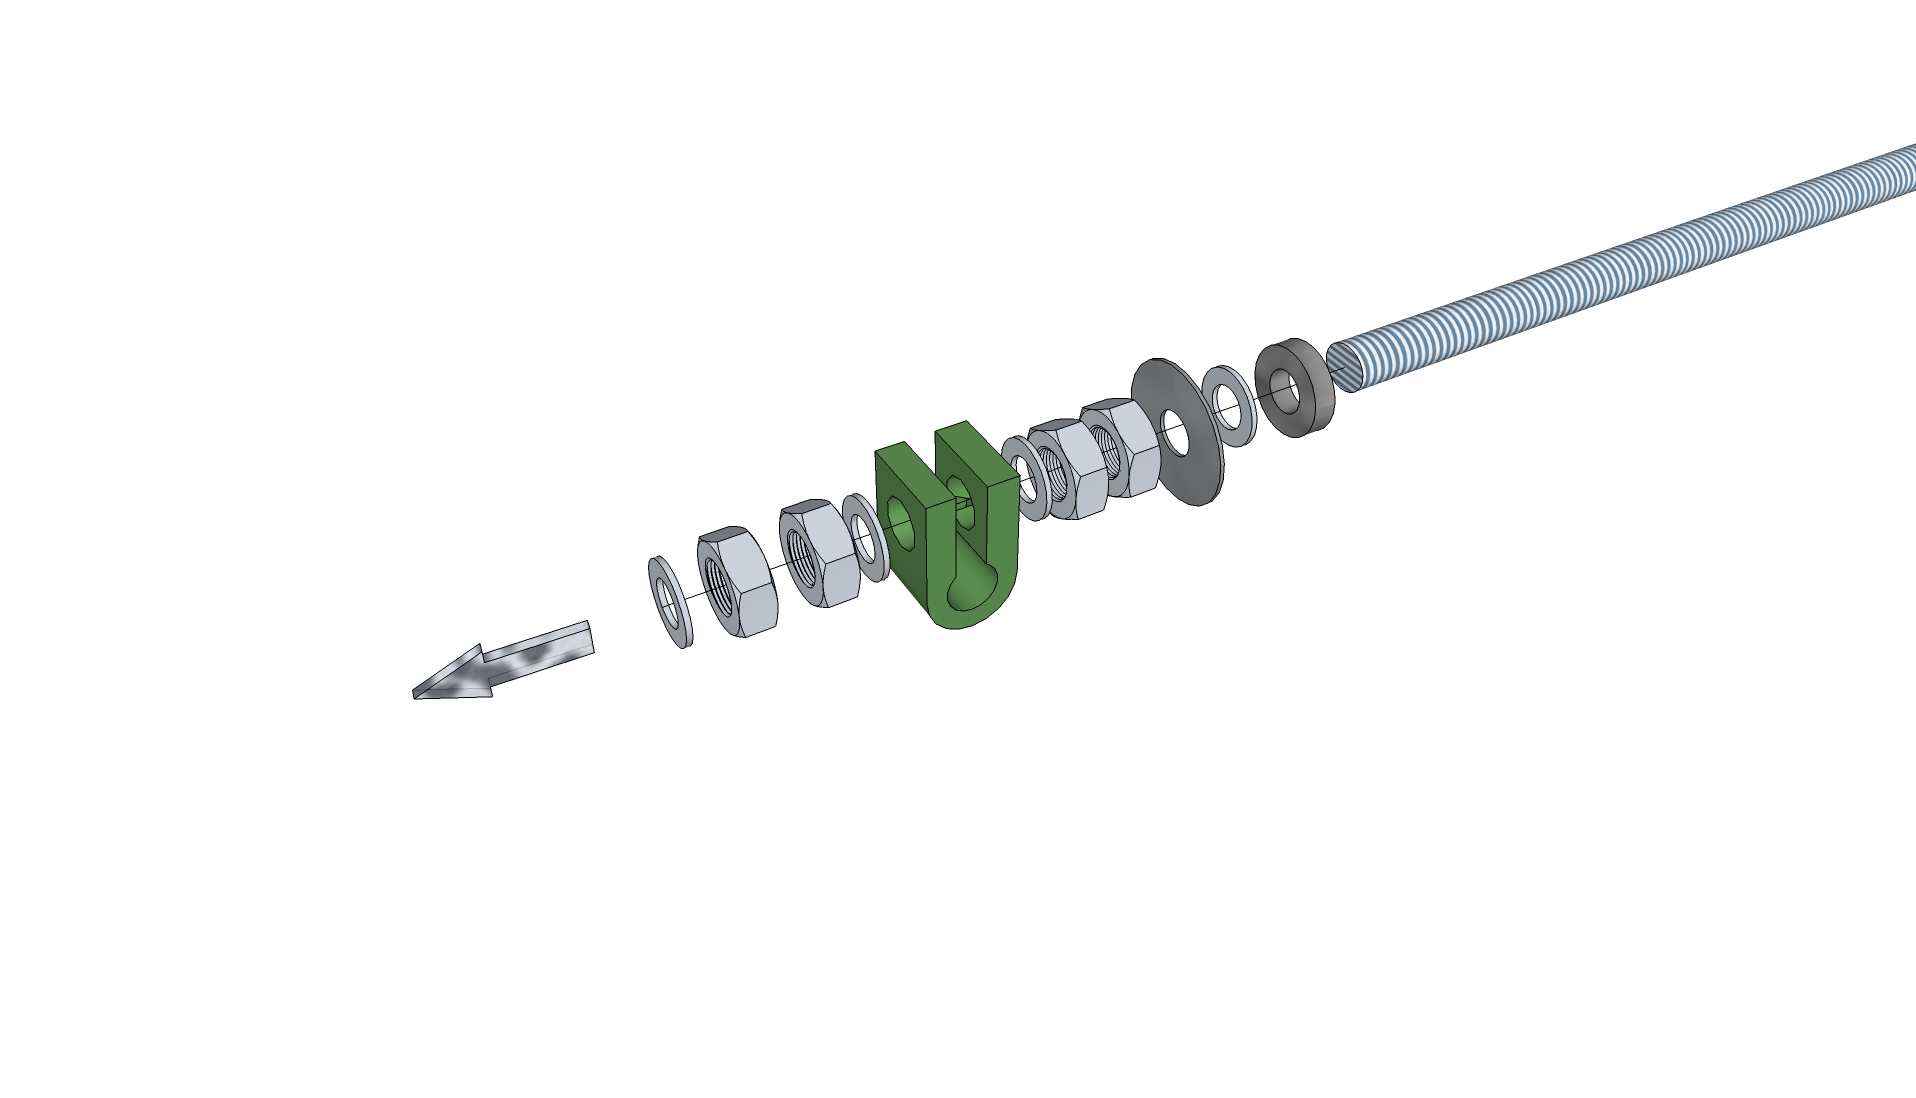
\includegraphics[width=1\linewidth]{graphics/ch3_2_1.png}
	[ Lefthand Side ]
	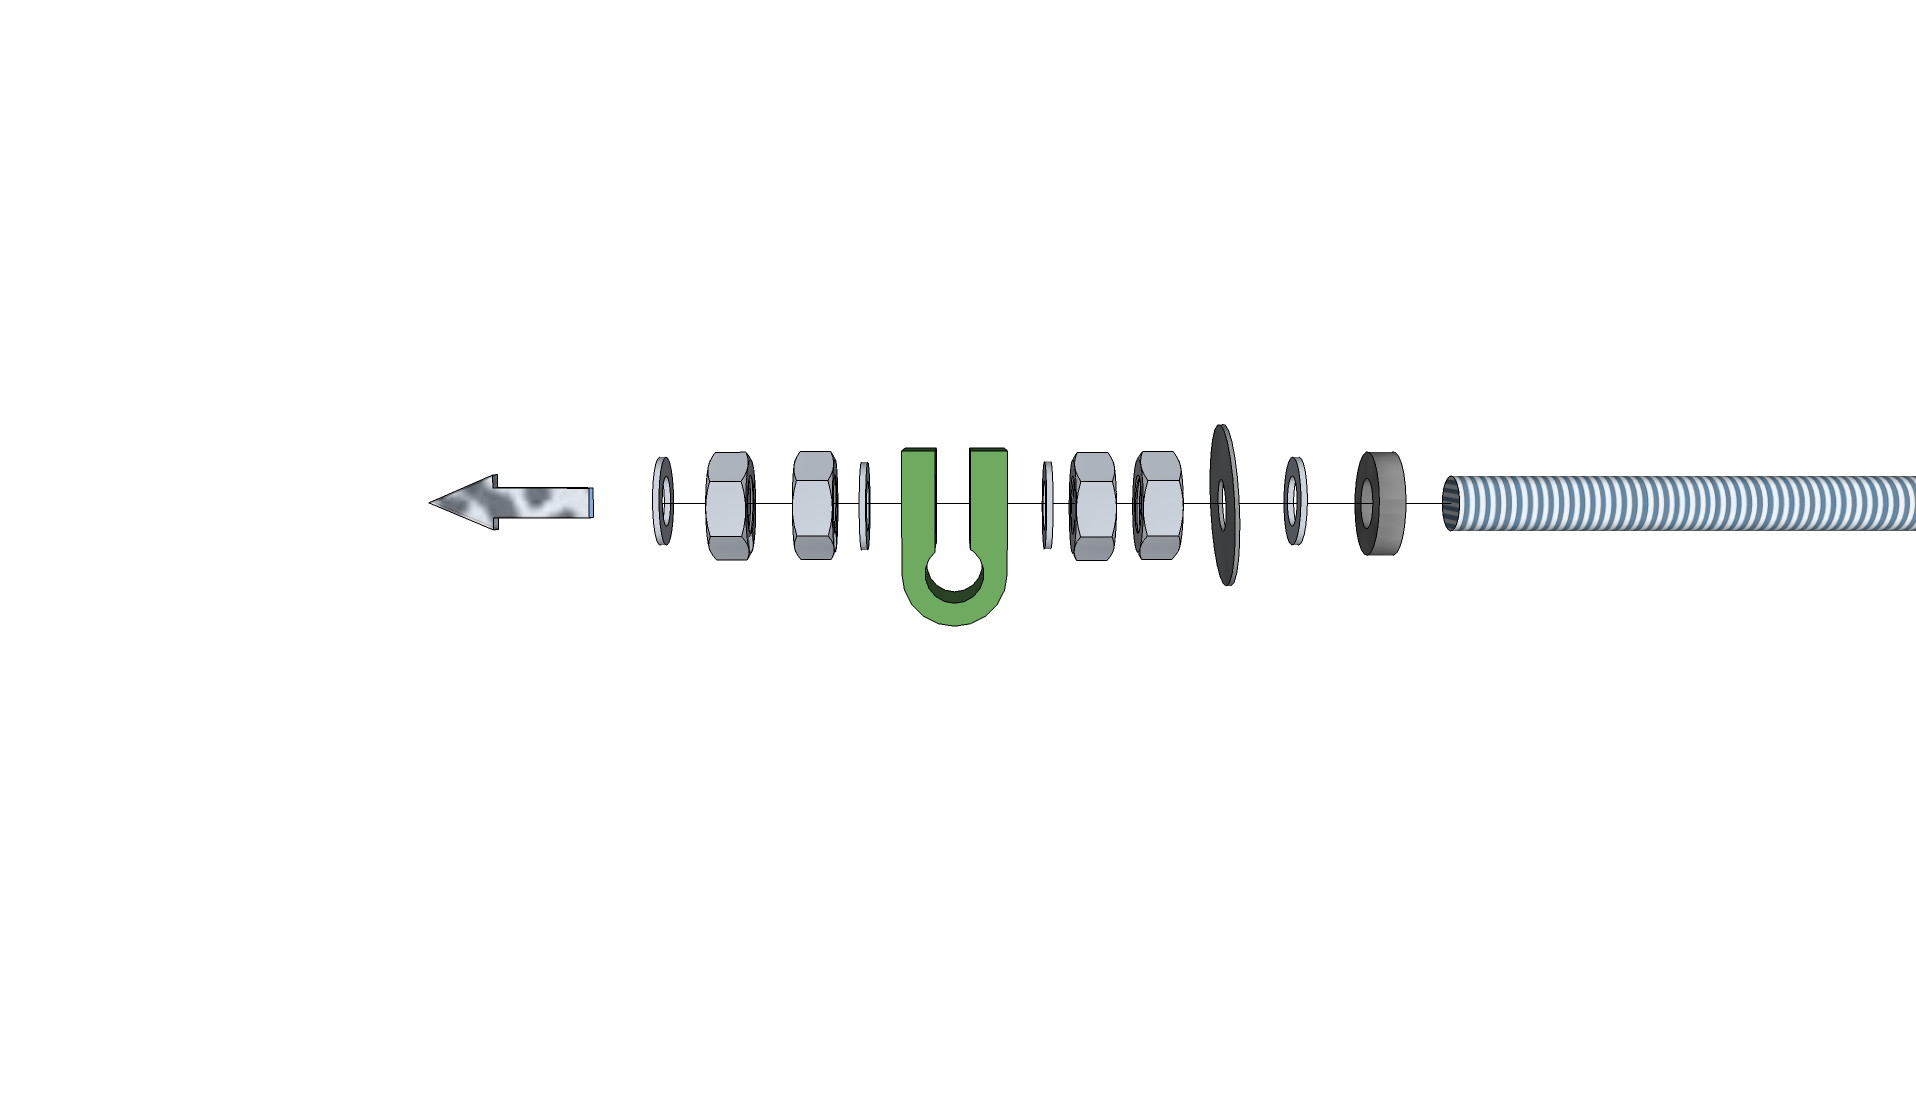
\includegraphics[width=1\linewidth]{graphics/ch3_2_2.png}
	[ Righthand Side ]
	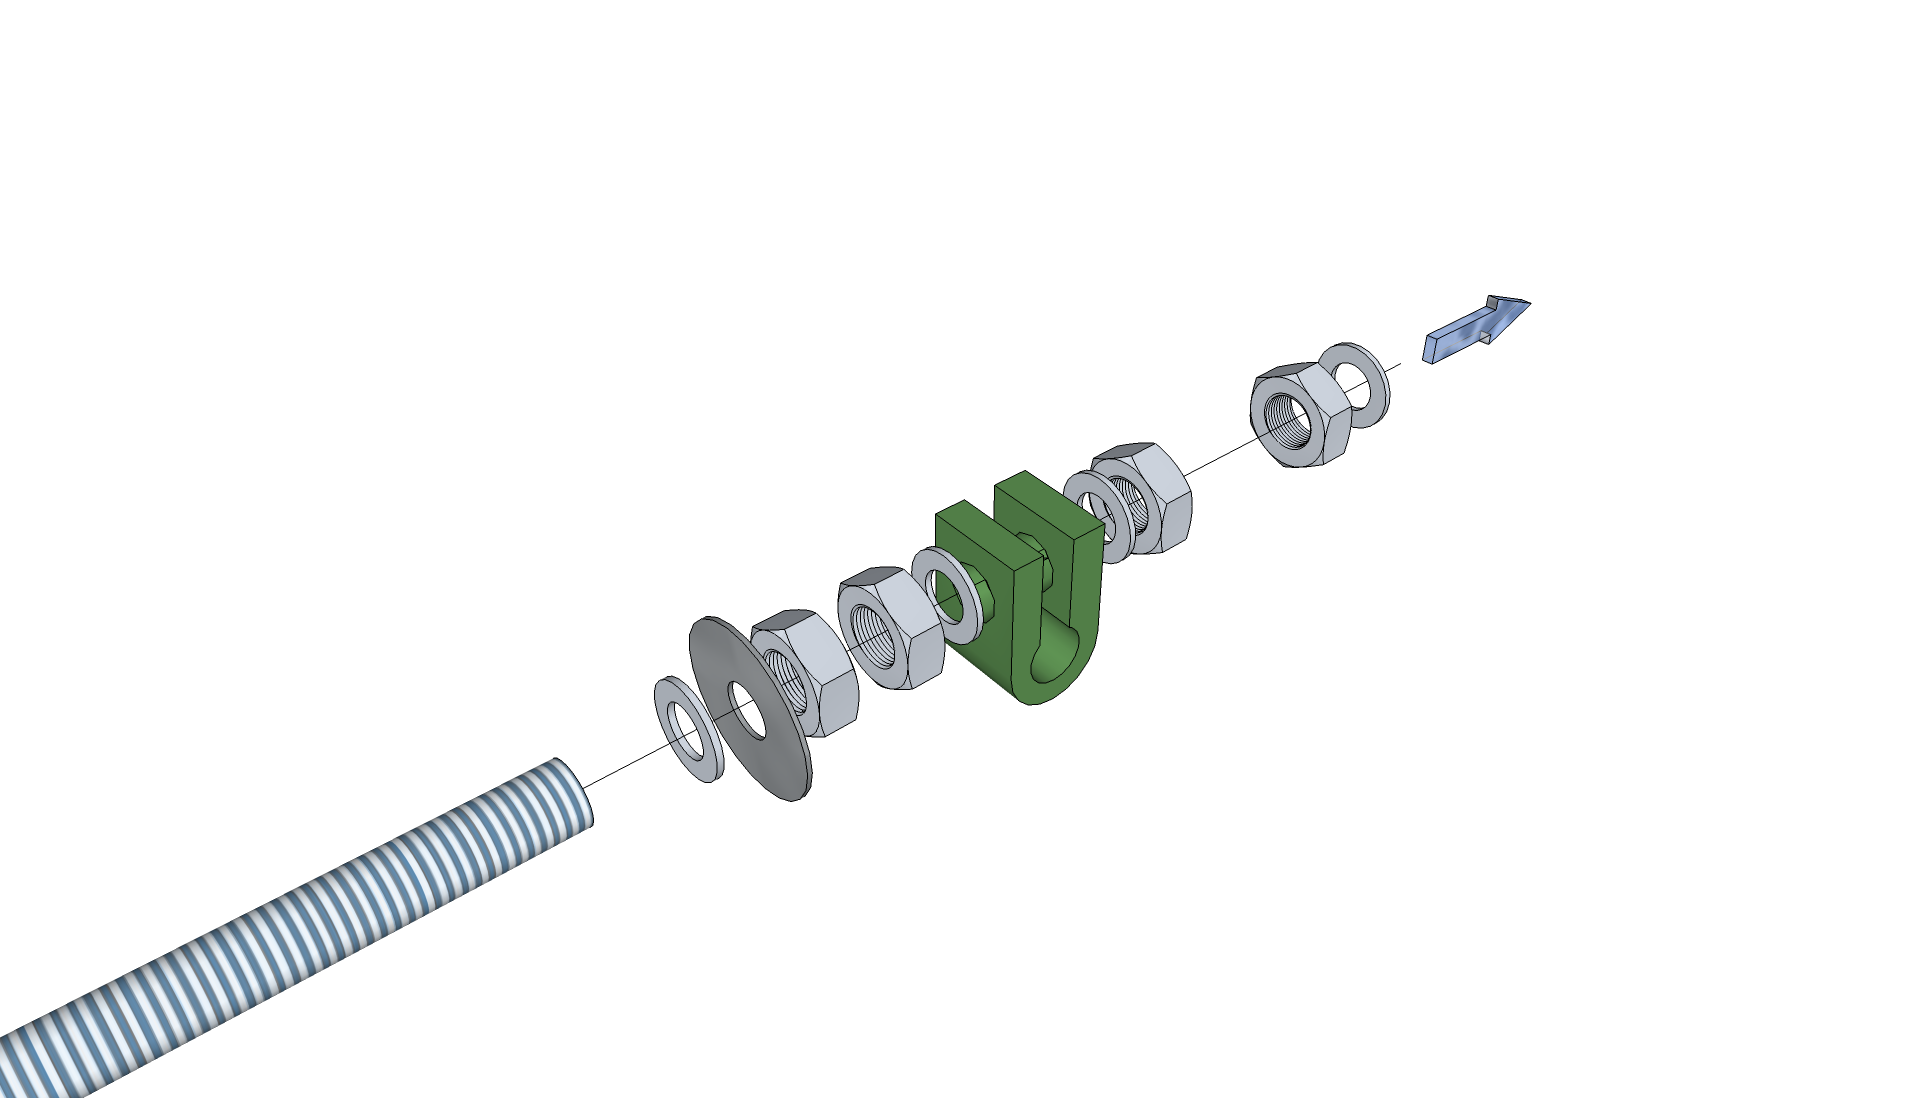
\includegraphics[width=1\linewidth]{graphics/ch3_2_3.png}
	
	\section{}
	It should look like the picture below. Verify this now.\\
	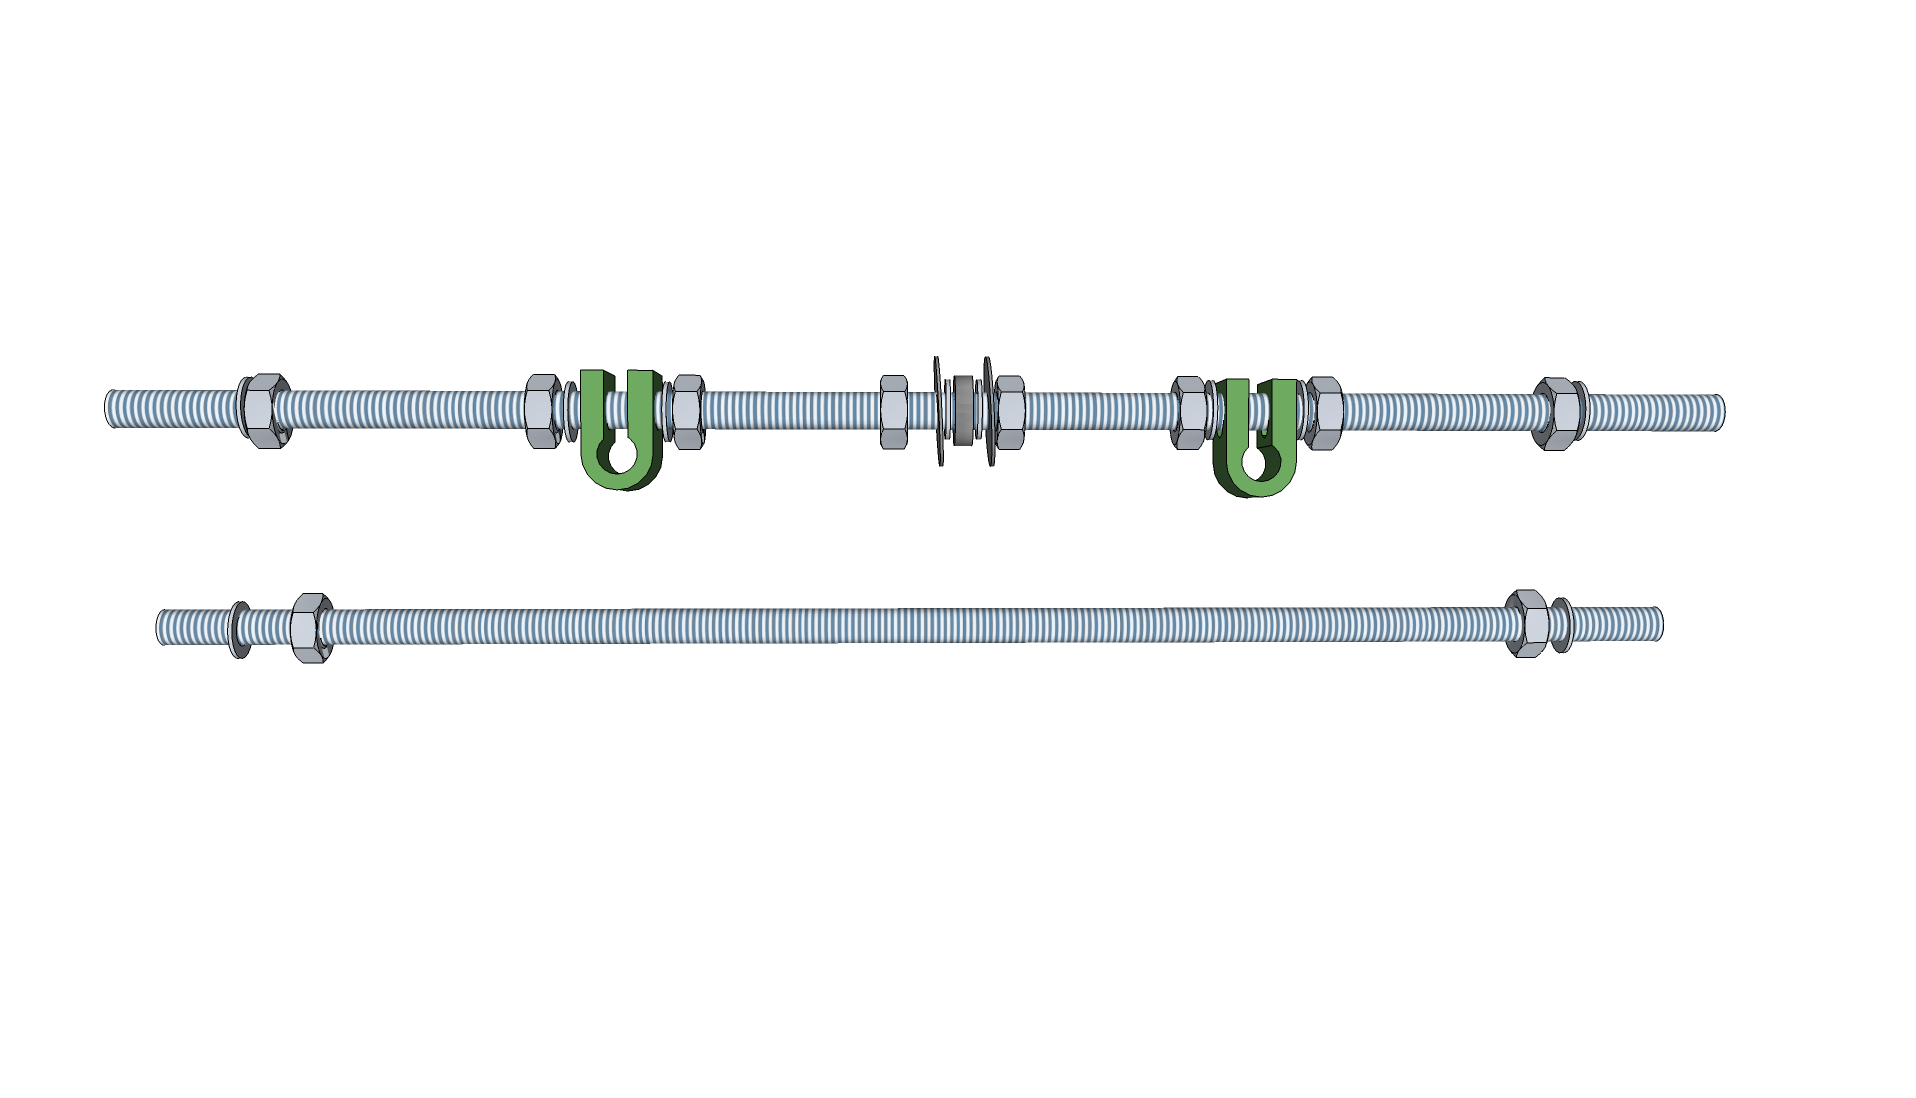
\includegraphics[width=1\linewidth]{graphics/ch3_3.png}
	
	\section{}
	Attach the two rods to the two remaining footed vertices. Thread each end of the rod through the vertex,
	and add a washer and nut. It should now look like this:
	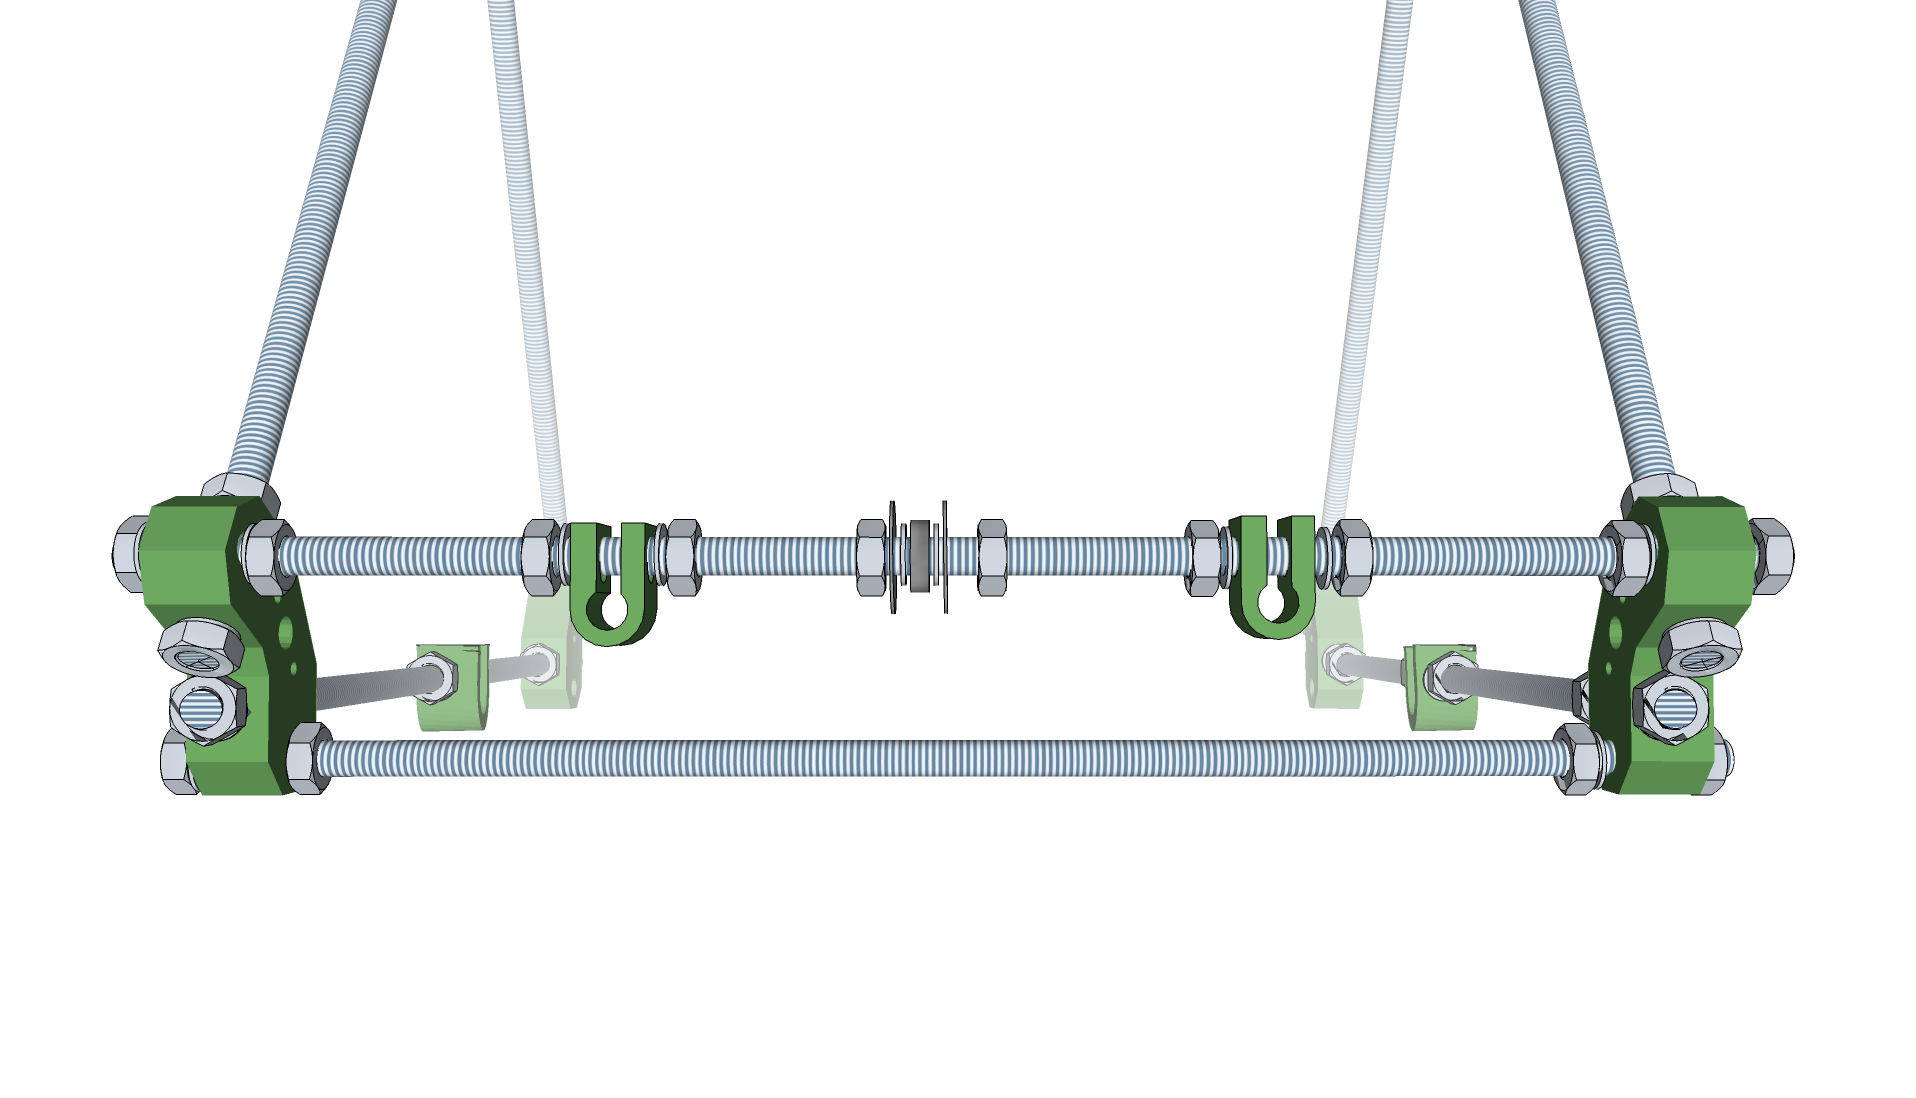
\includegraphics[width=1\linewidth]{graphics/ch3_4_1.png}
	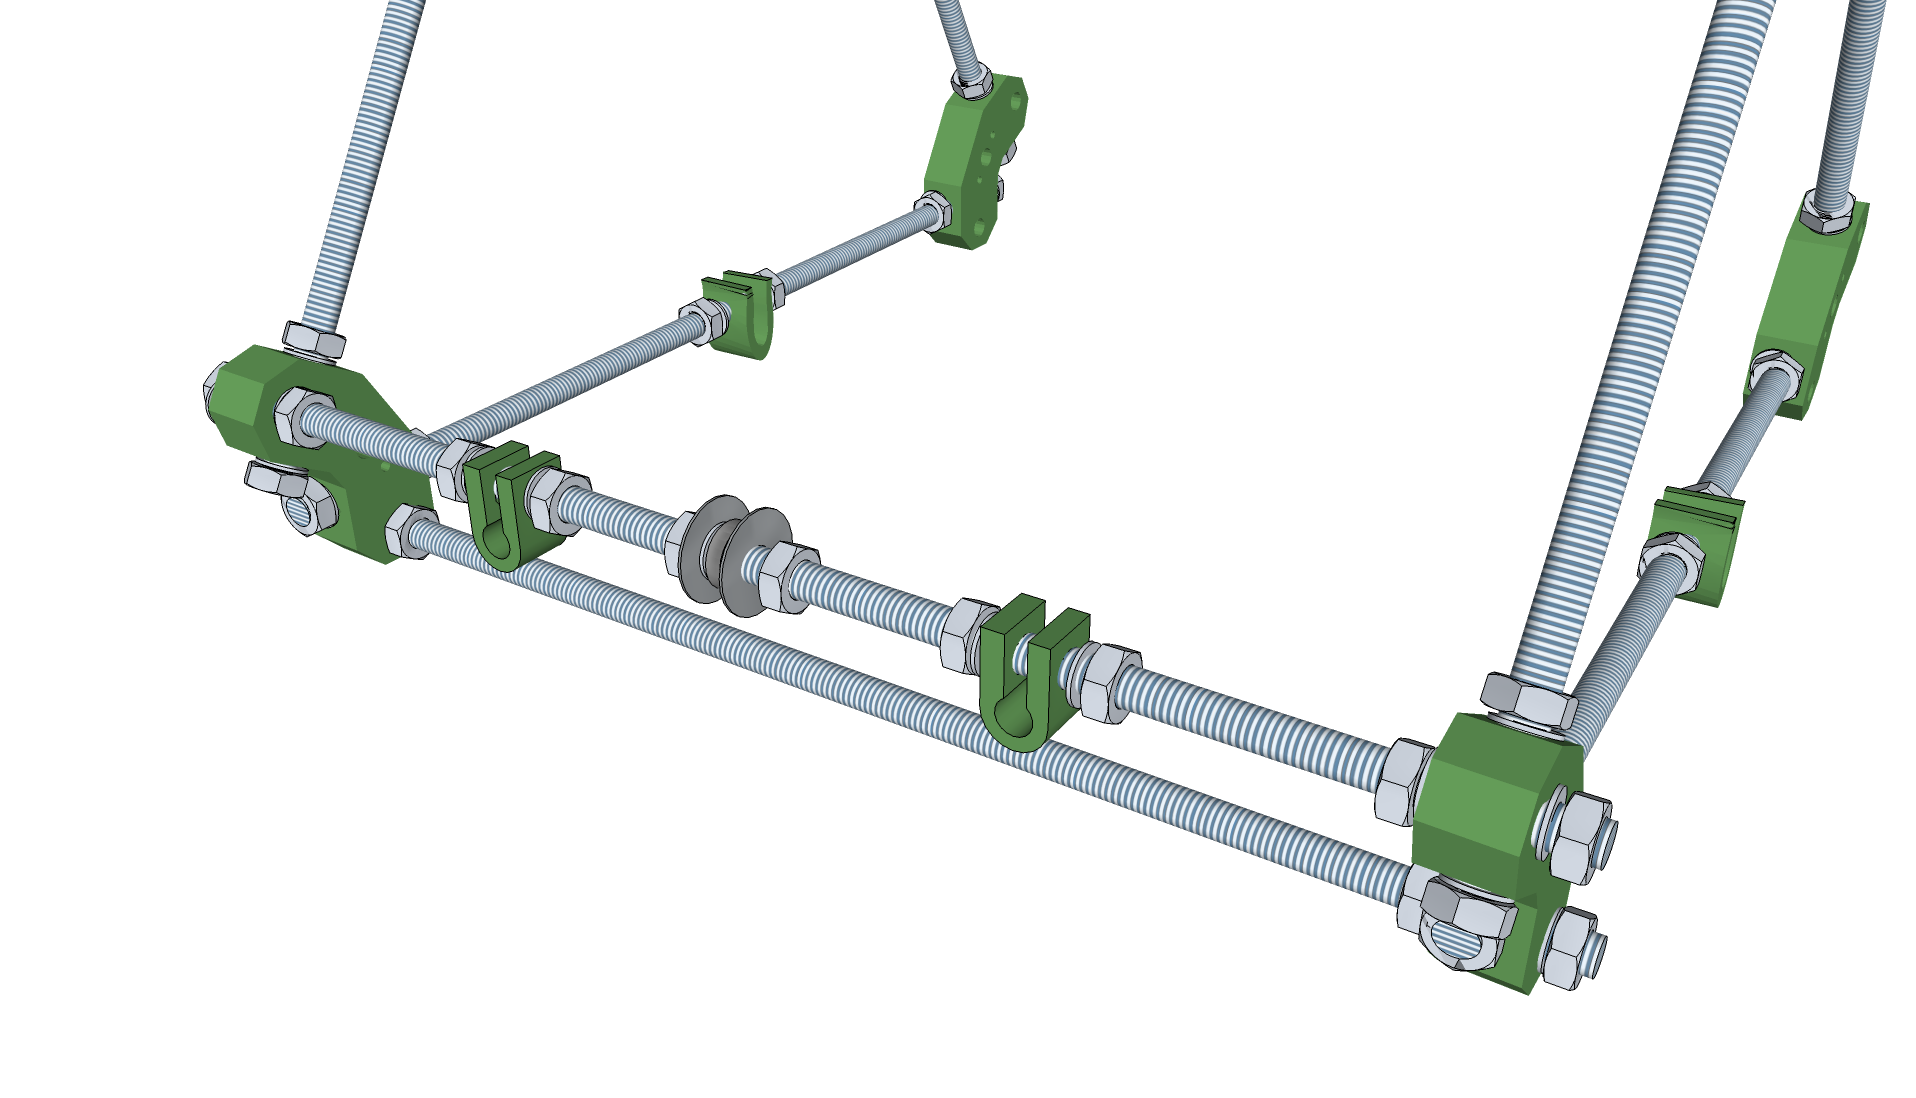
\includegraphics[width=1\linewidth]{graphics/ch3_4_2.png}
	
	\section{}
	Your frame should now be standing on its own feet without support, but the tops sides of the triangles
	will still be wobbly. We'll fix that next.\\
	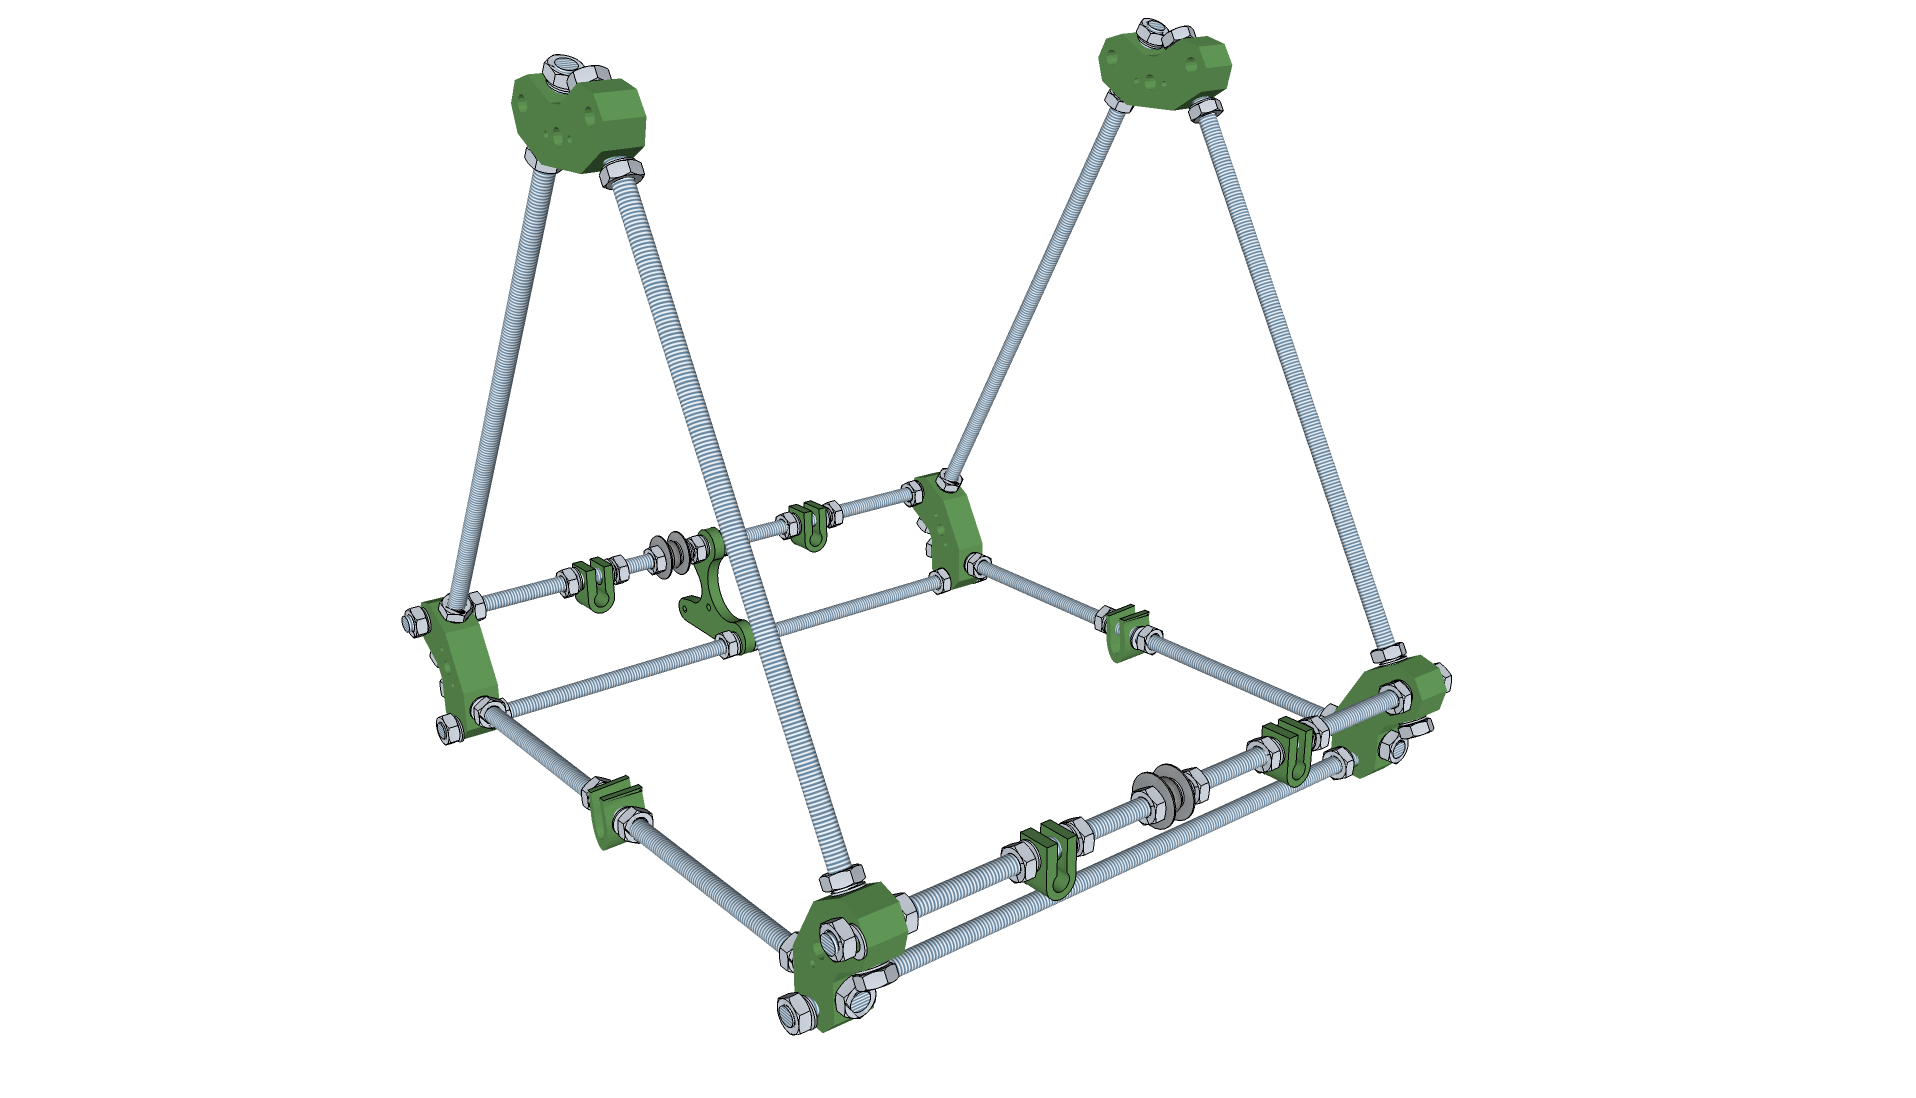
\includegraphics[width=1\linewidth]{graphics/ch3_5.png}
	
	\chapter{Assembling the top threaded rods}
	
	\section{}
	Slide one of the threaded rods through one side of one of the top vertices. Put a washer, two nuts, and
	another washer on the part of the rod between the top vertices.\\
	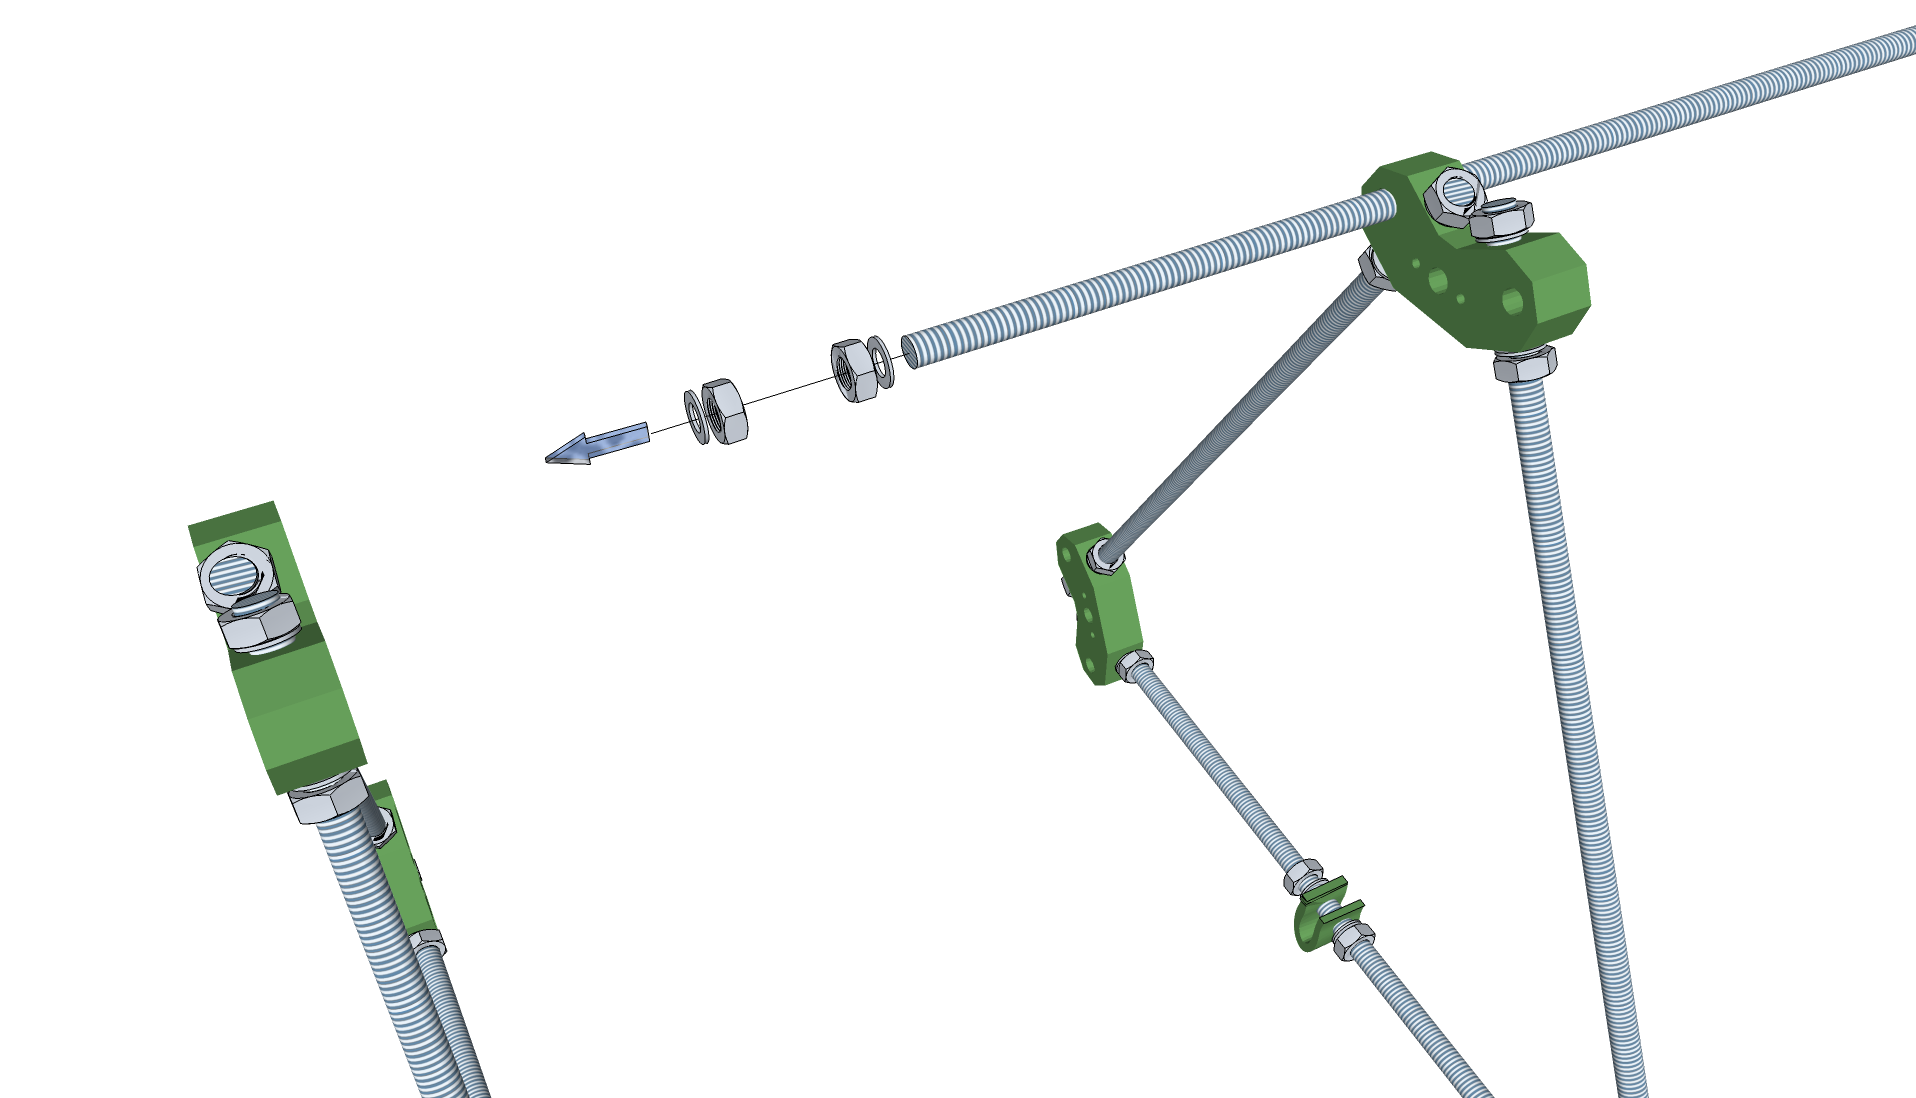
\includegraphics[width=1\linewidth]{graphics/ch4_1.png}
	
	\section{}
	Repeat for the other rod.\\
	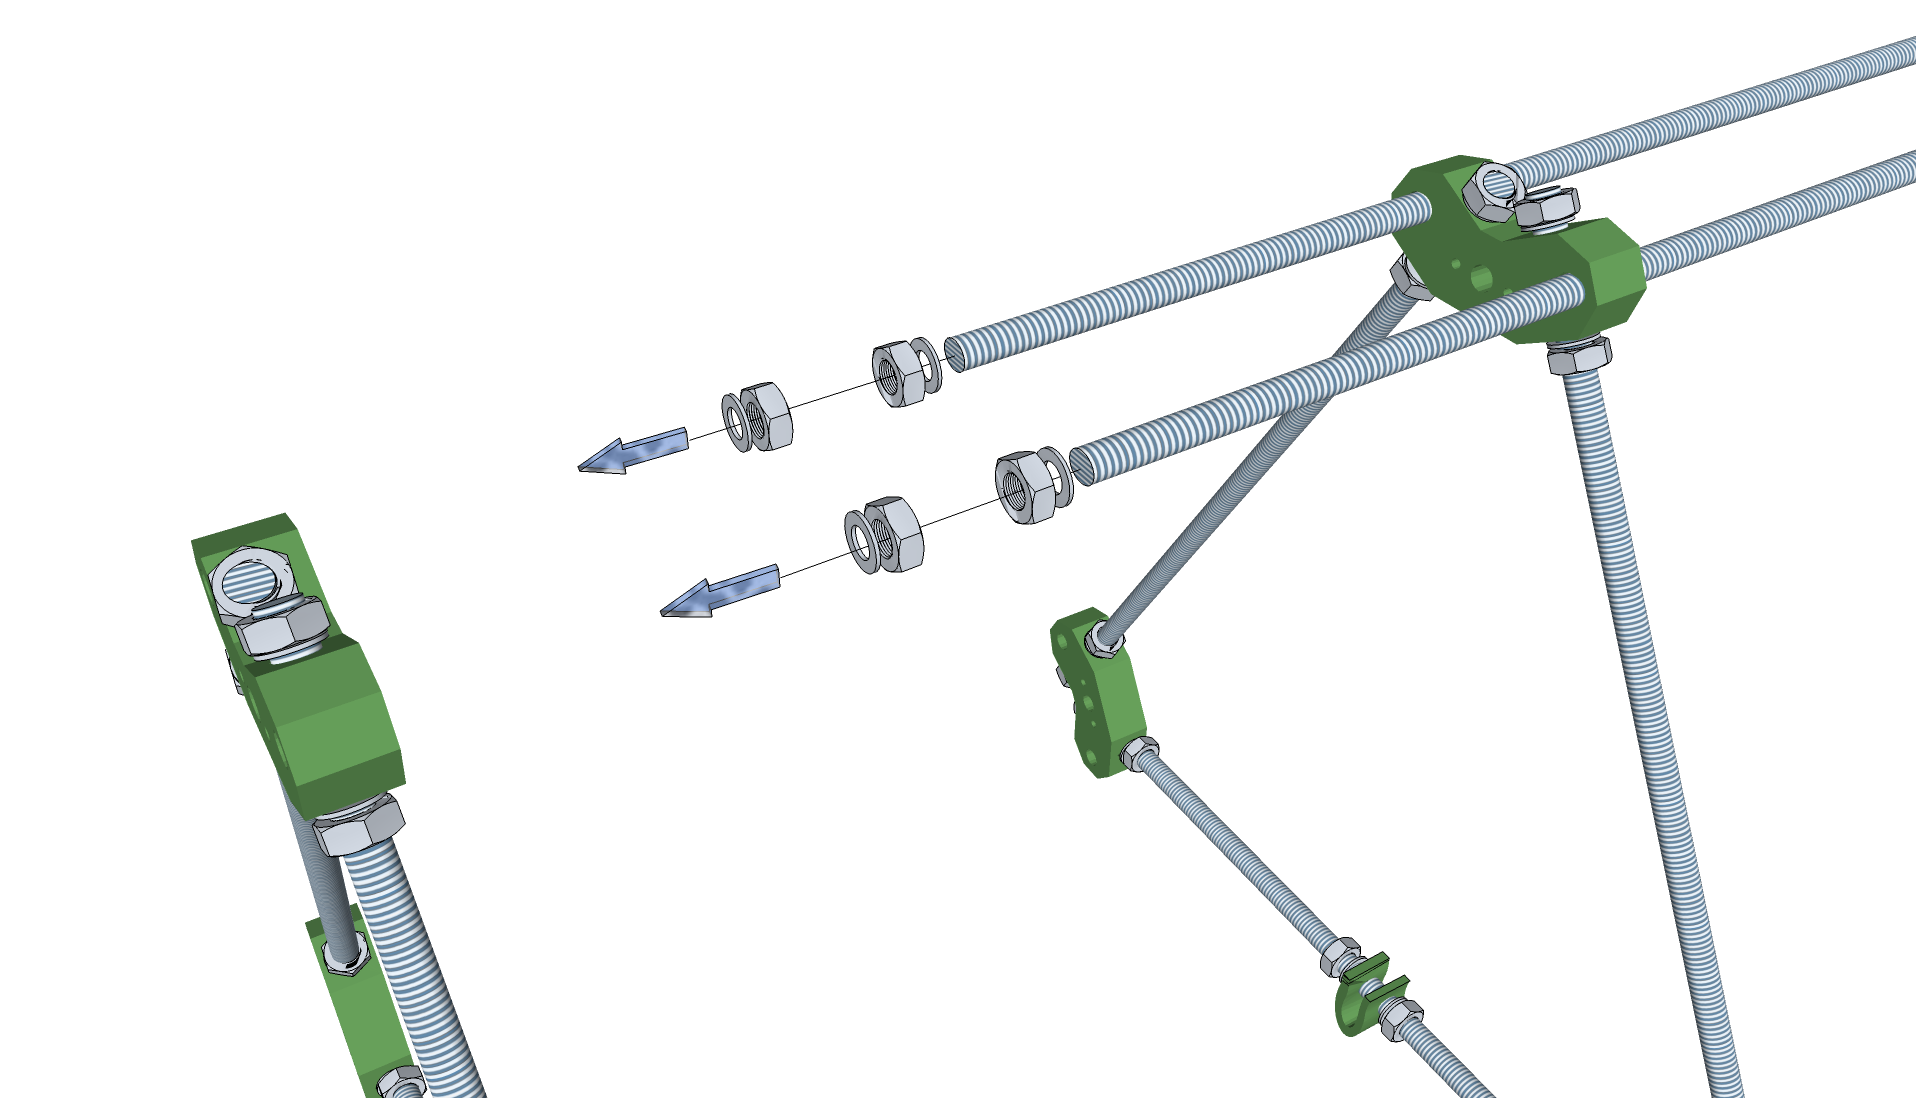
\includegraphics[width=1\linewidth]{graphics/ch4_2_1.png}
	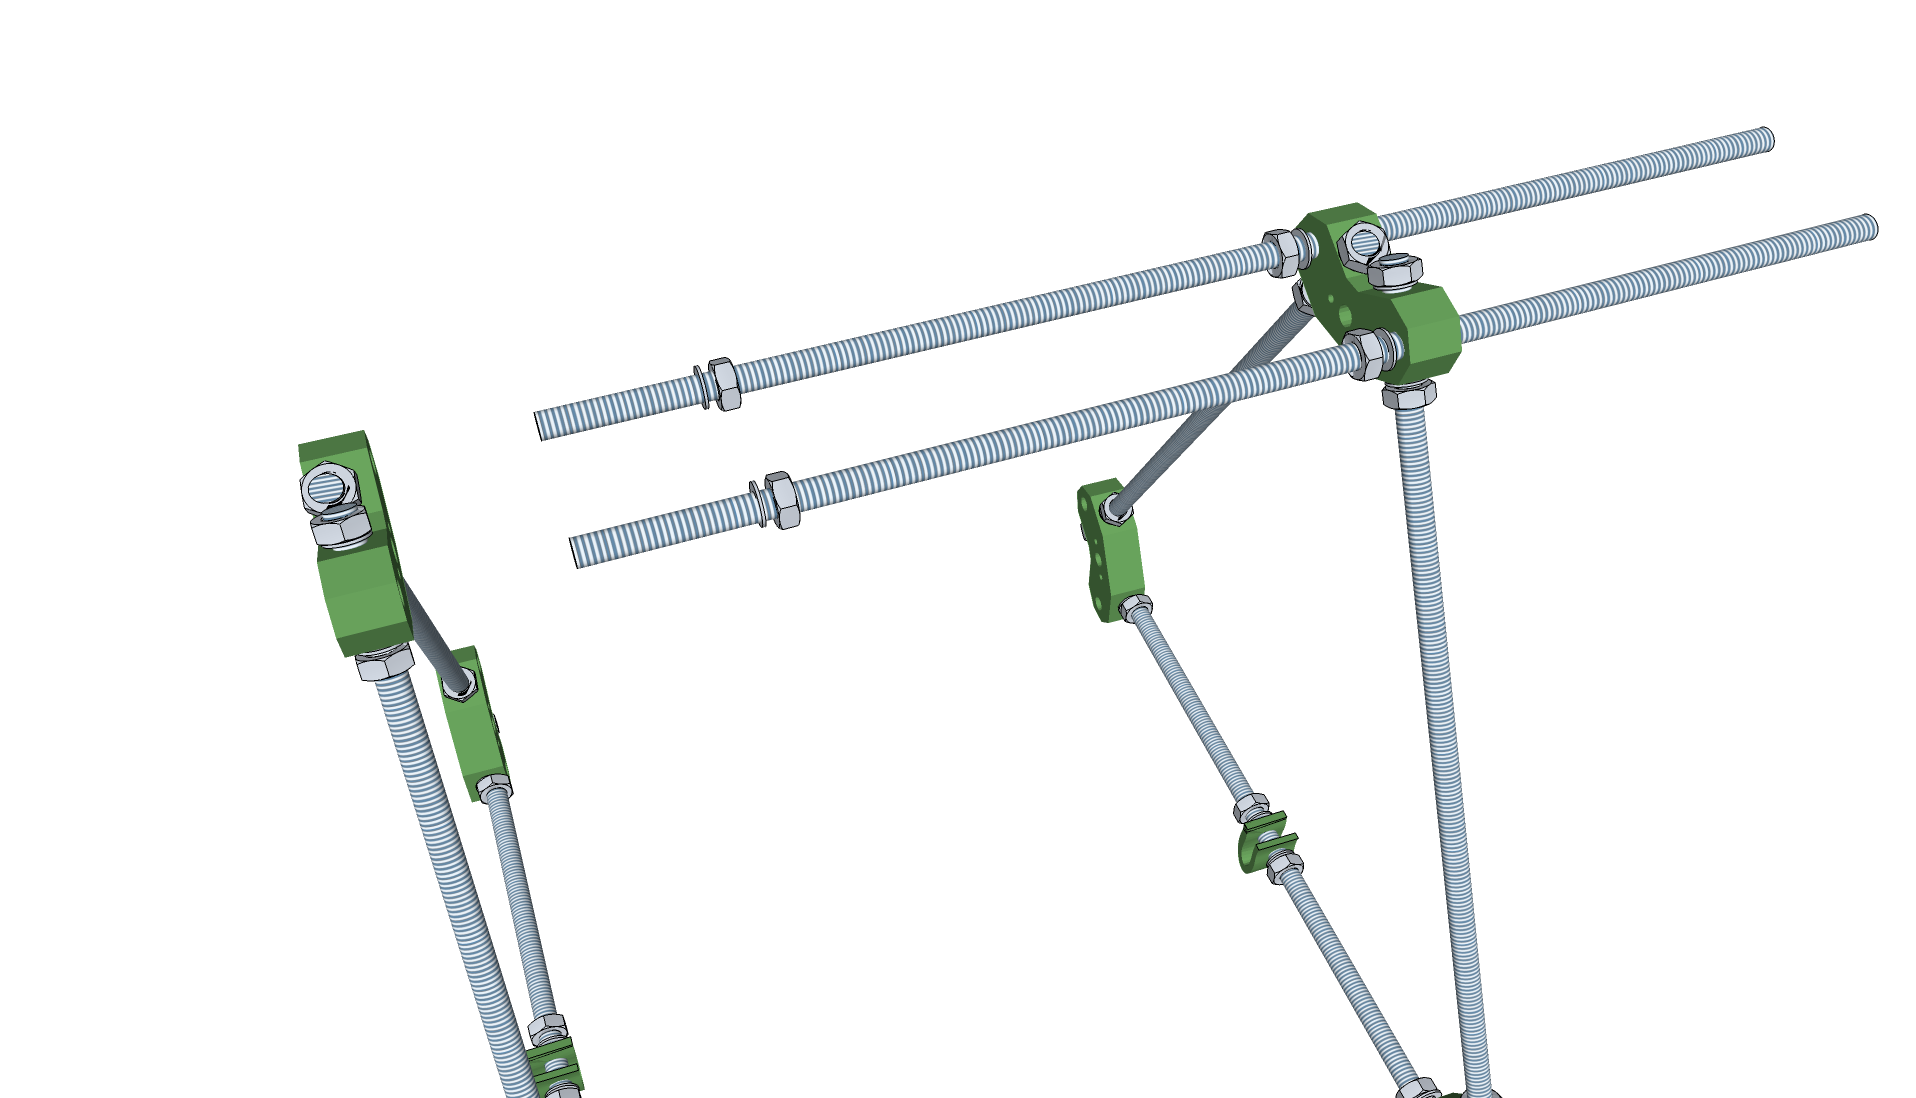
\includegraphics[width=1\linewidth]{graphics/ch4_2_2.png}
	
	\section{}
	Slide the rods through the opposite side vertex. Thread the nuts up to the vertices on each side.\\
	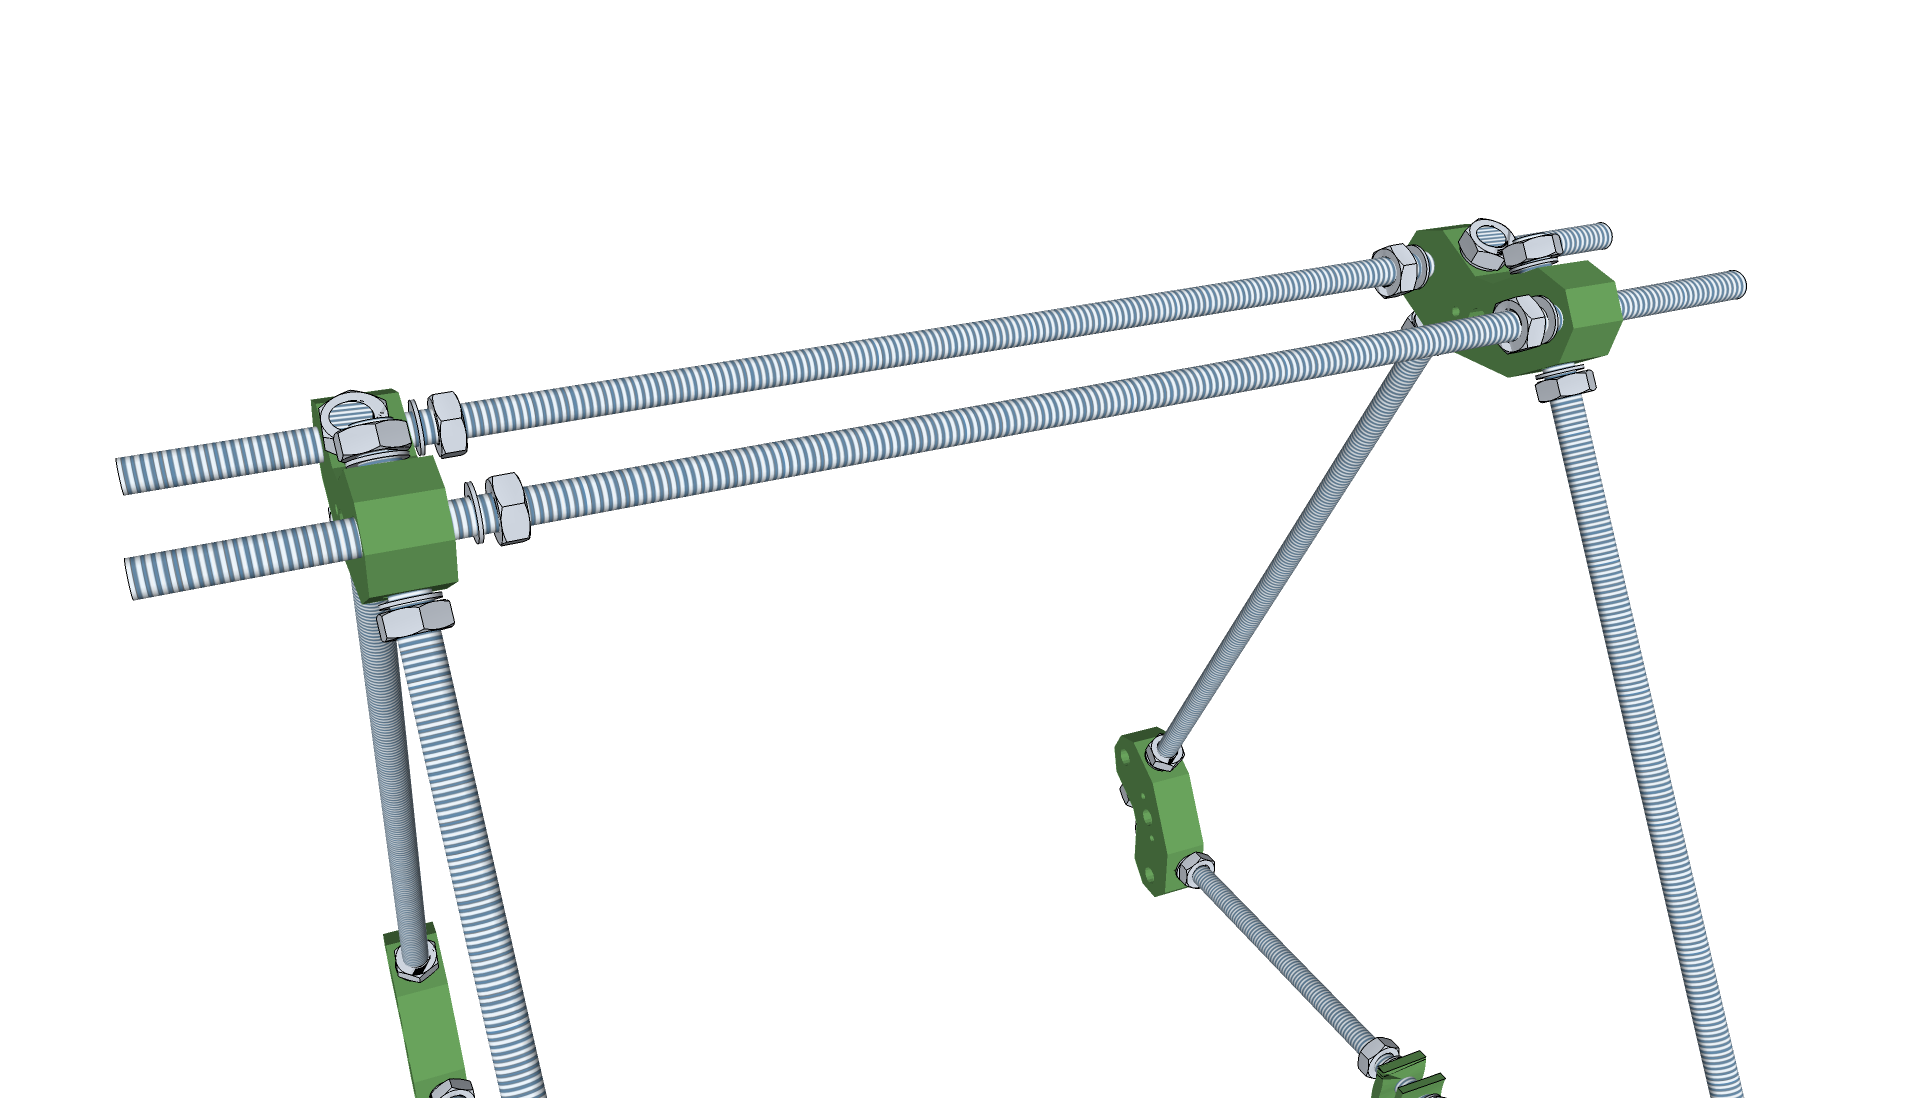
\includegraphics[width=1\linewidth]{graphics/ch4_3.png}
	
	\section{}
	To each of the four ends of the threaded rod, add a washer, a nut and another washer.\\
	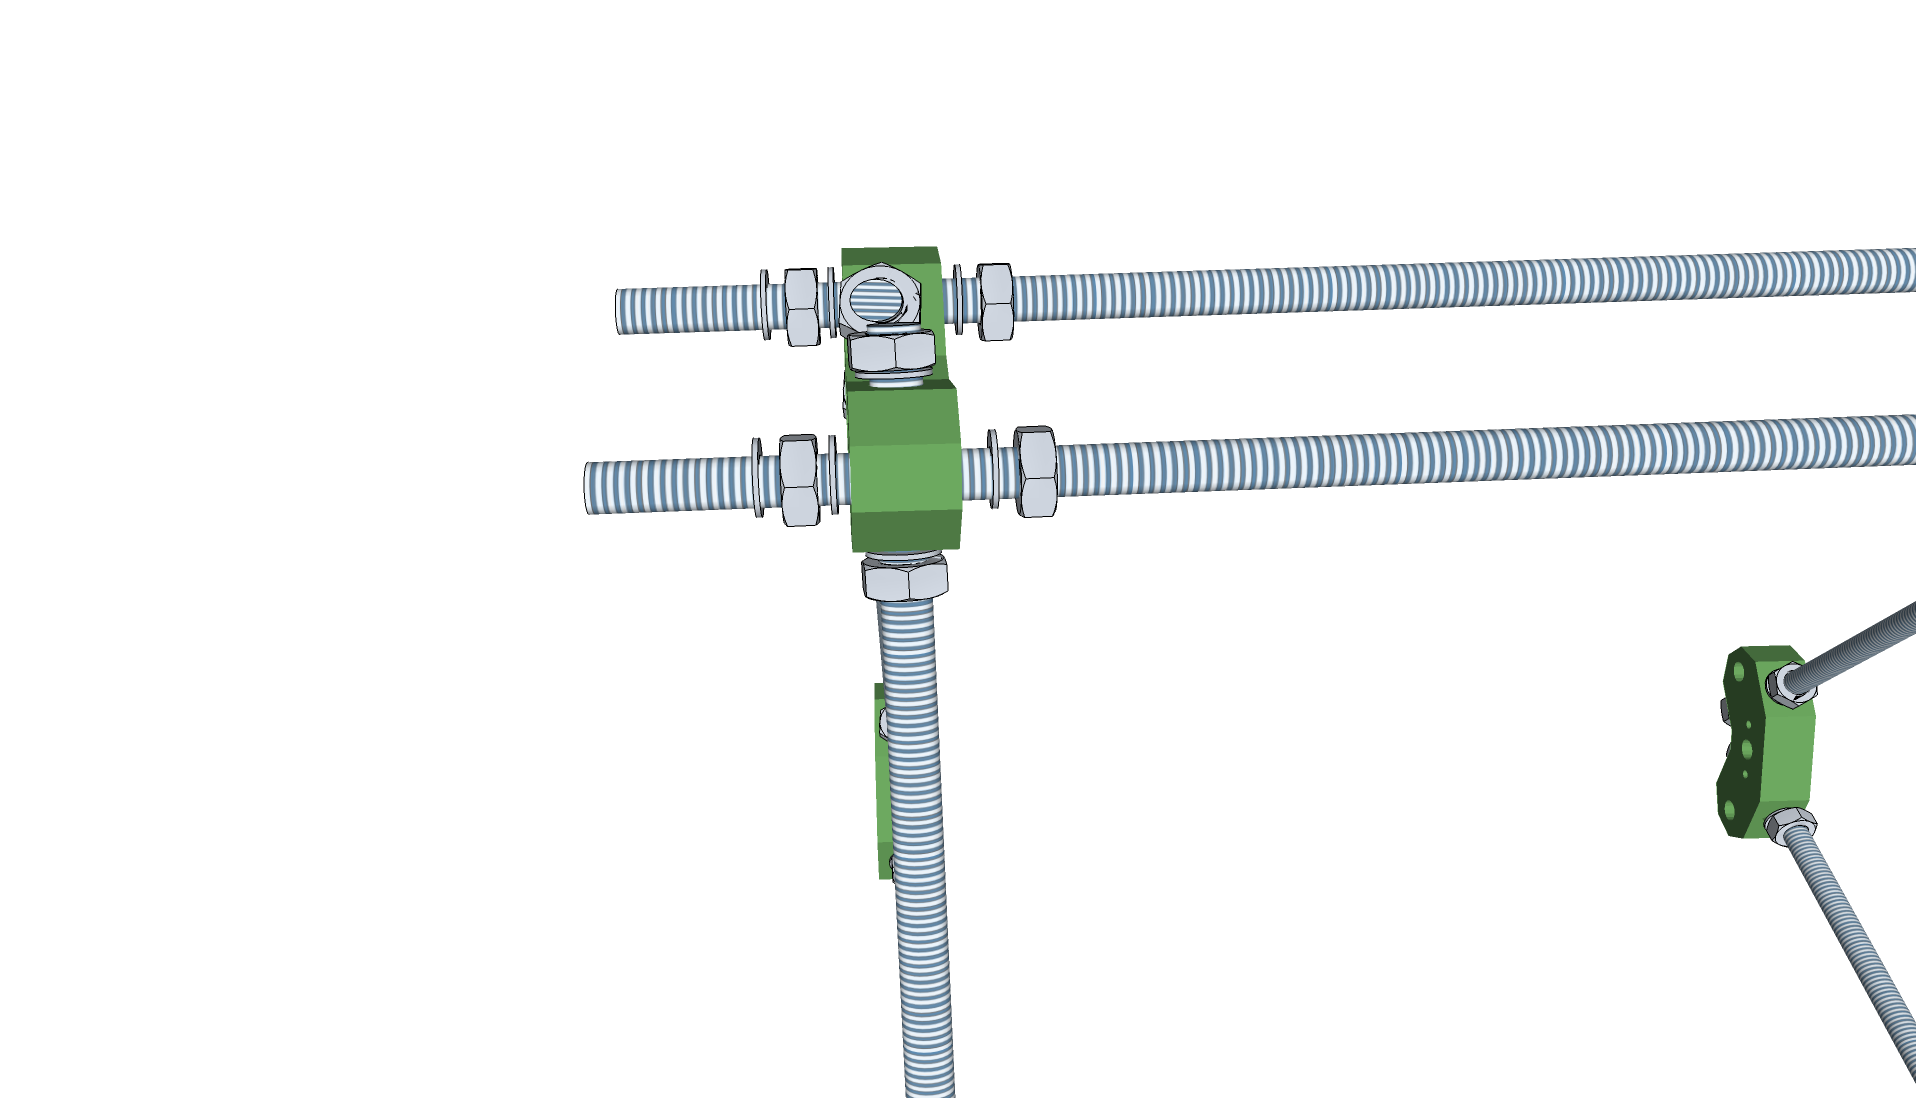
\includegraphics[width=1\linewidth]{graphics/ch4_4_1.png}
	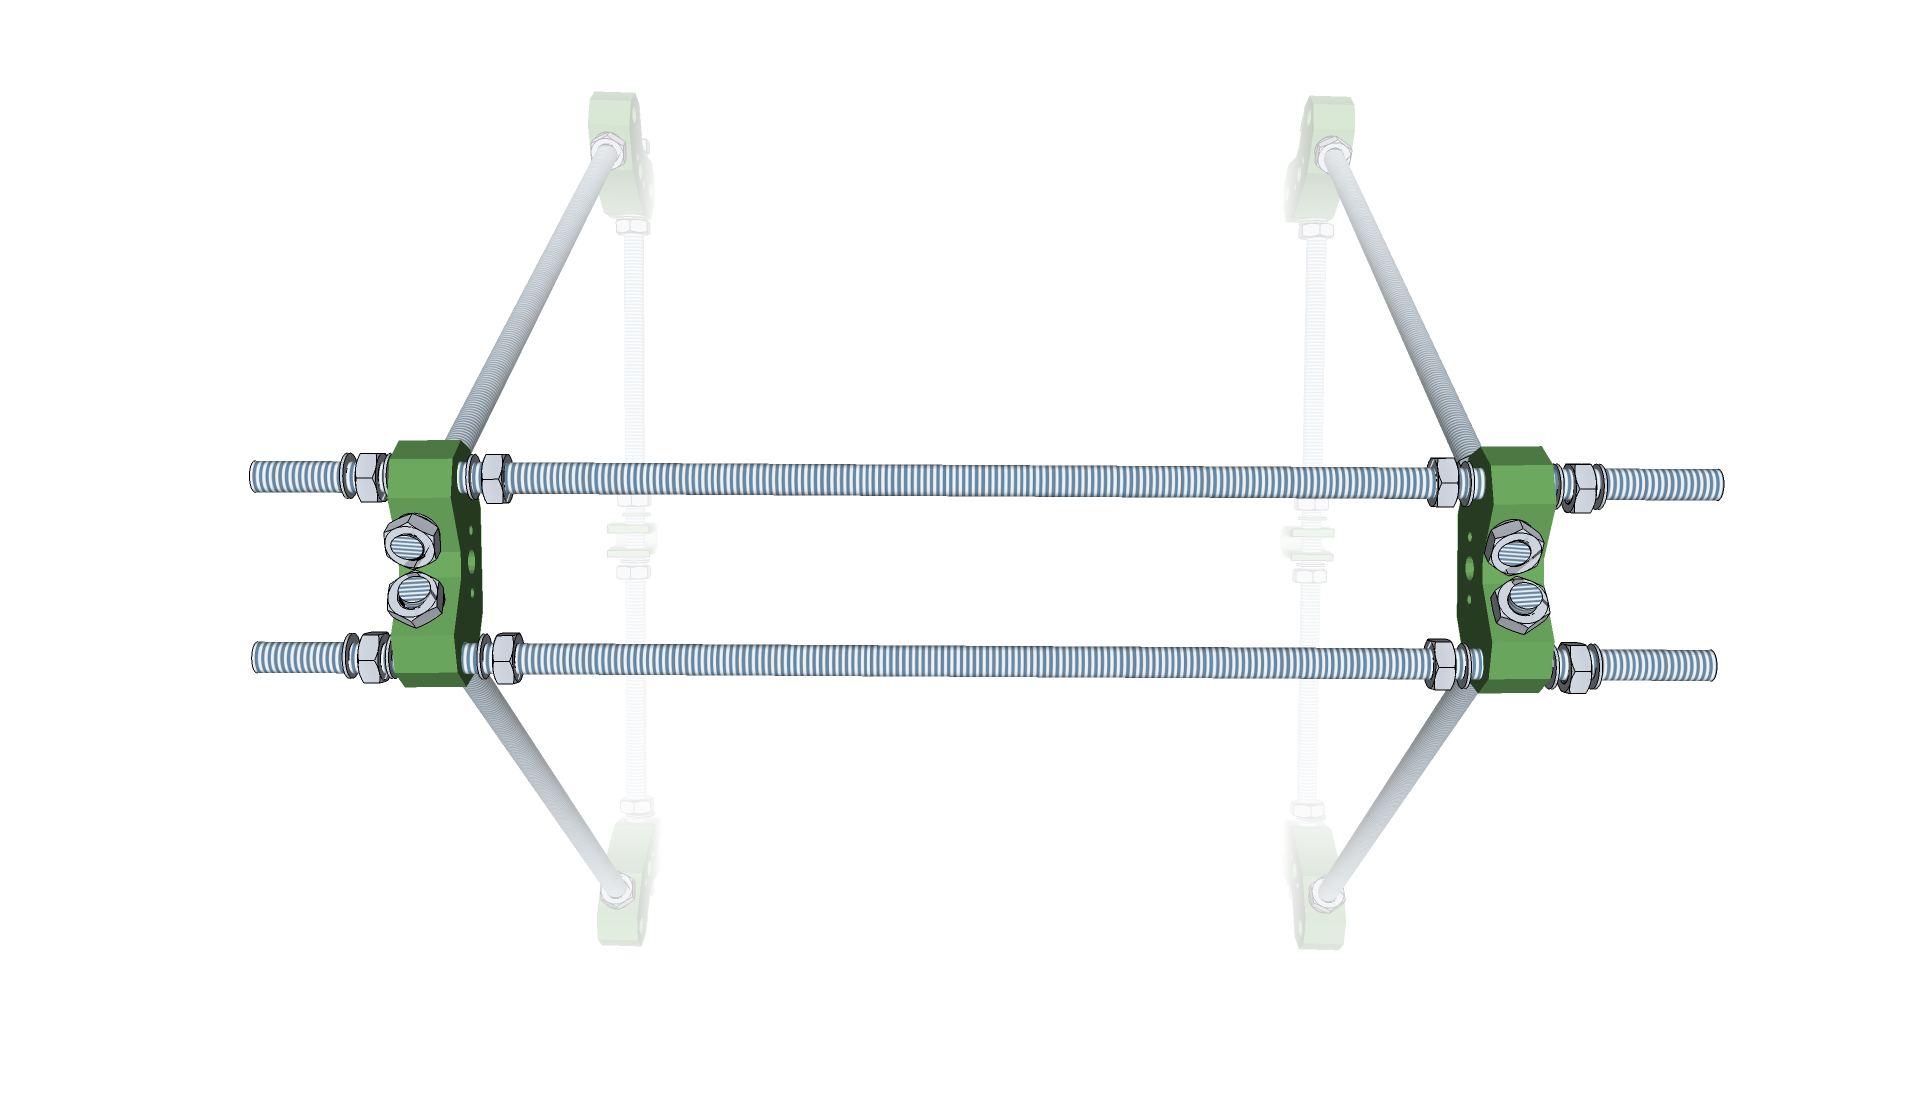
\includegraphics[width=1\linewidth]{graphics/ch4_4_2.png}
	
	\section{}
	Take one of the RP z motor mounts and attach it to the ends of the threaded rod. The side with the two
	holes and the indentation should point towards the outside. Add a washer and nut to the end of each
	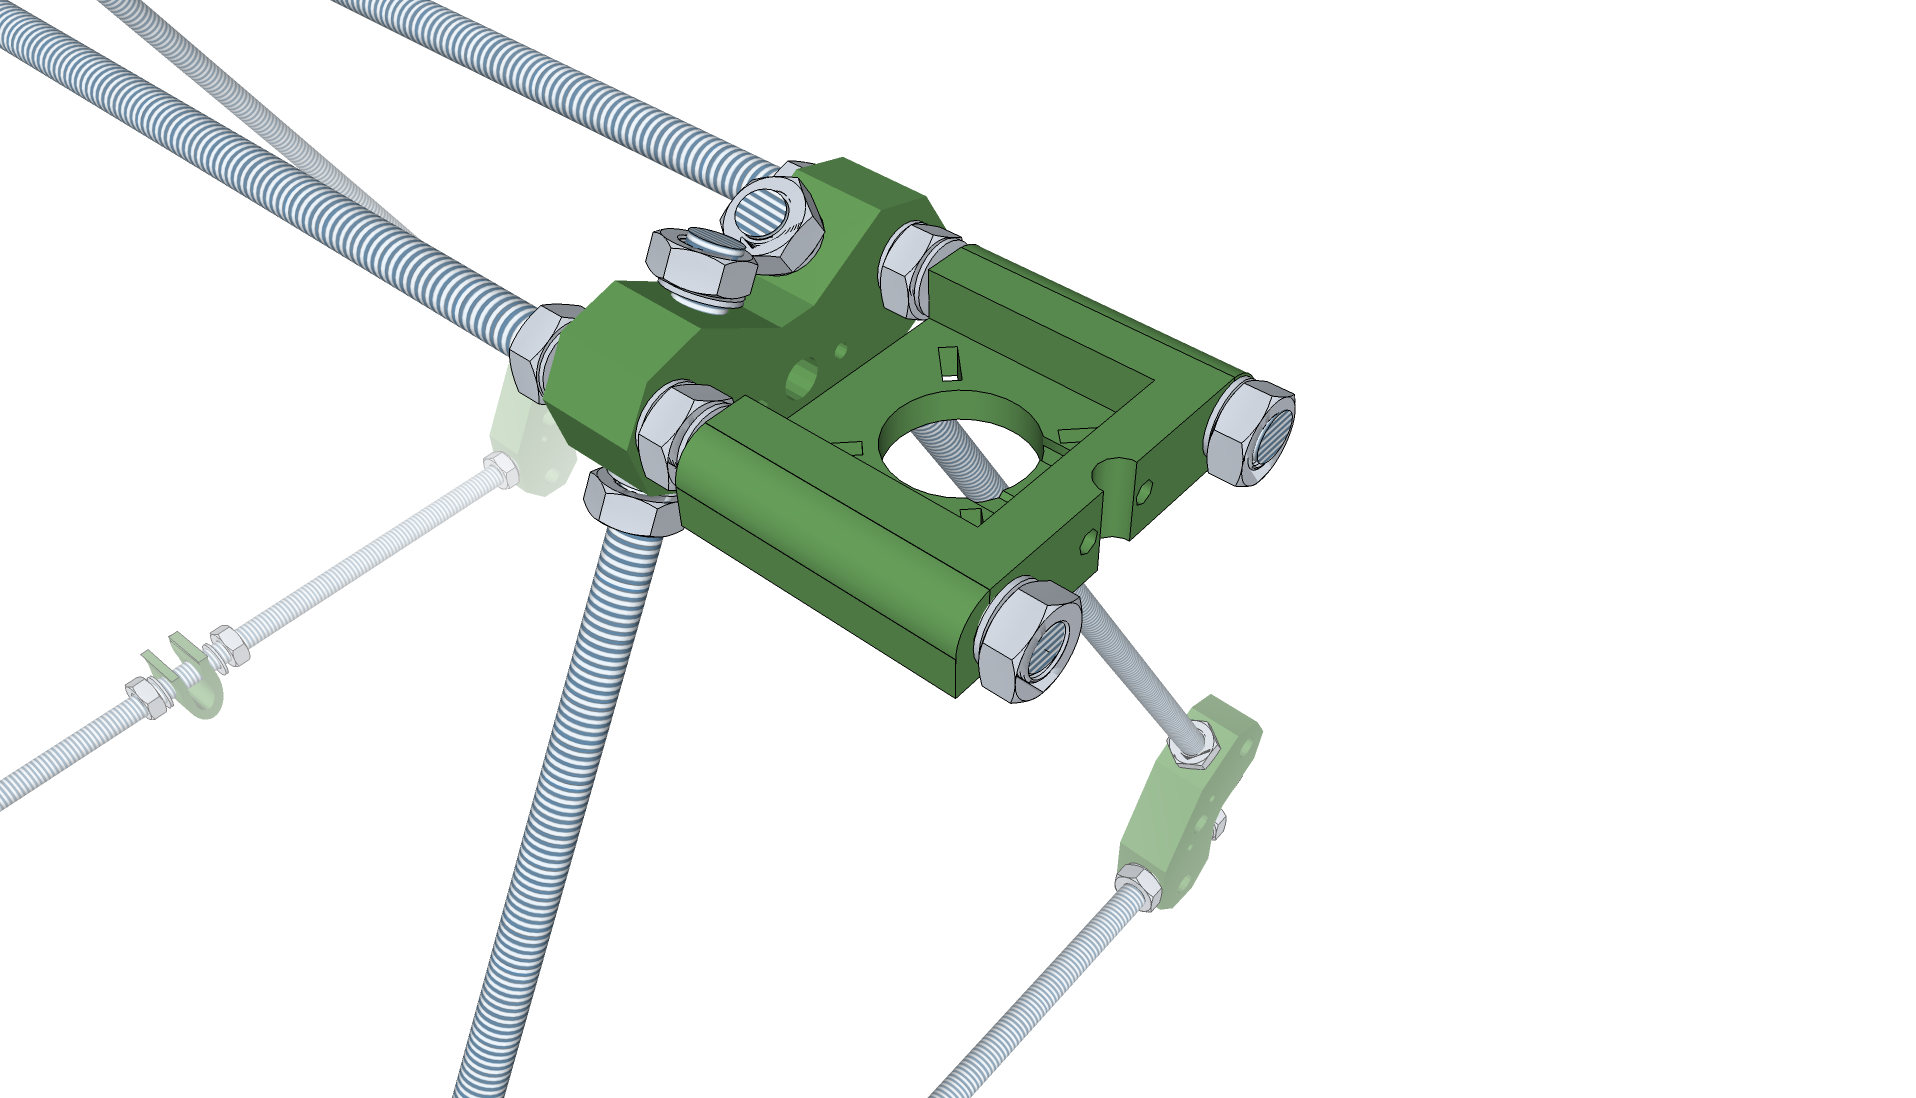
\includegraphics[width=1\linewidth]{graphics/ch4_5_1.png}
	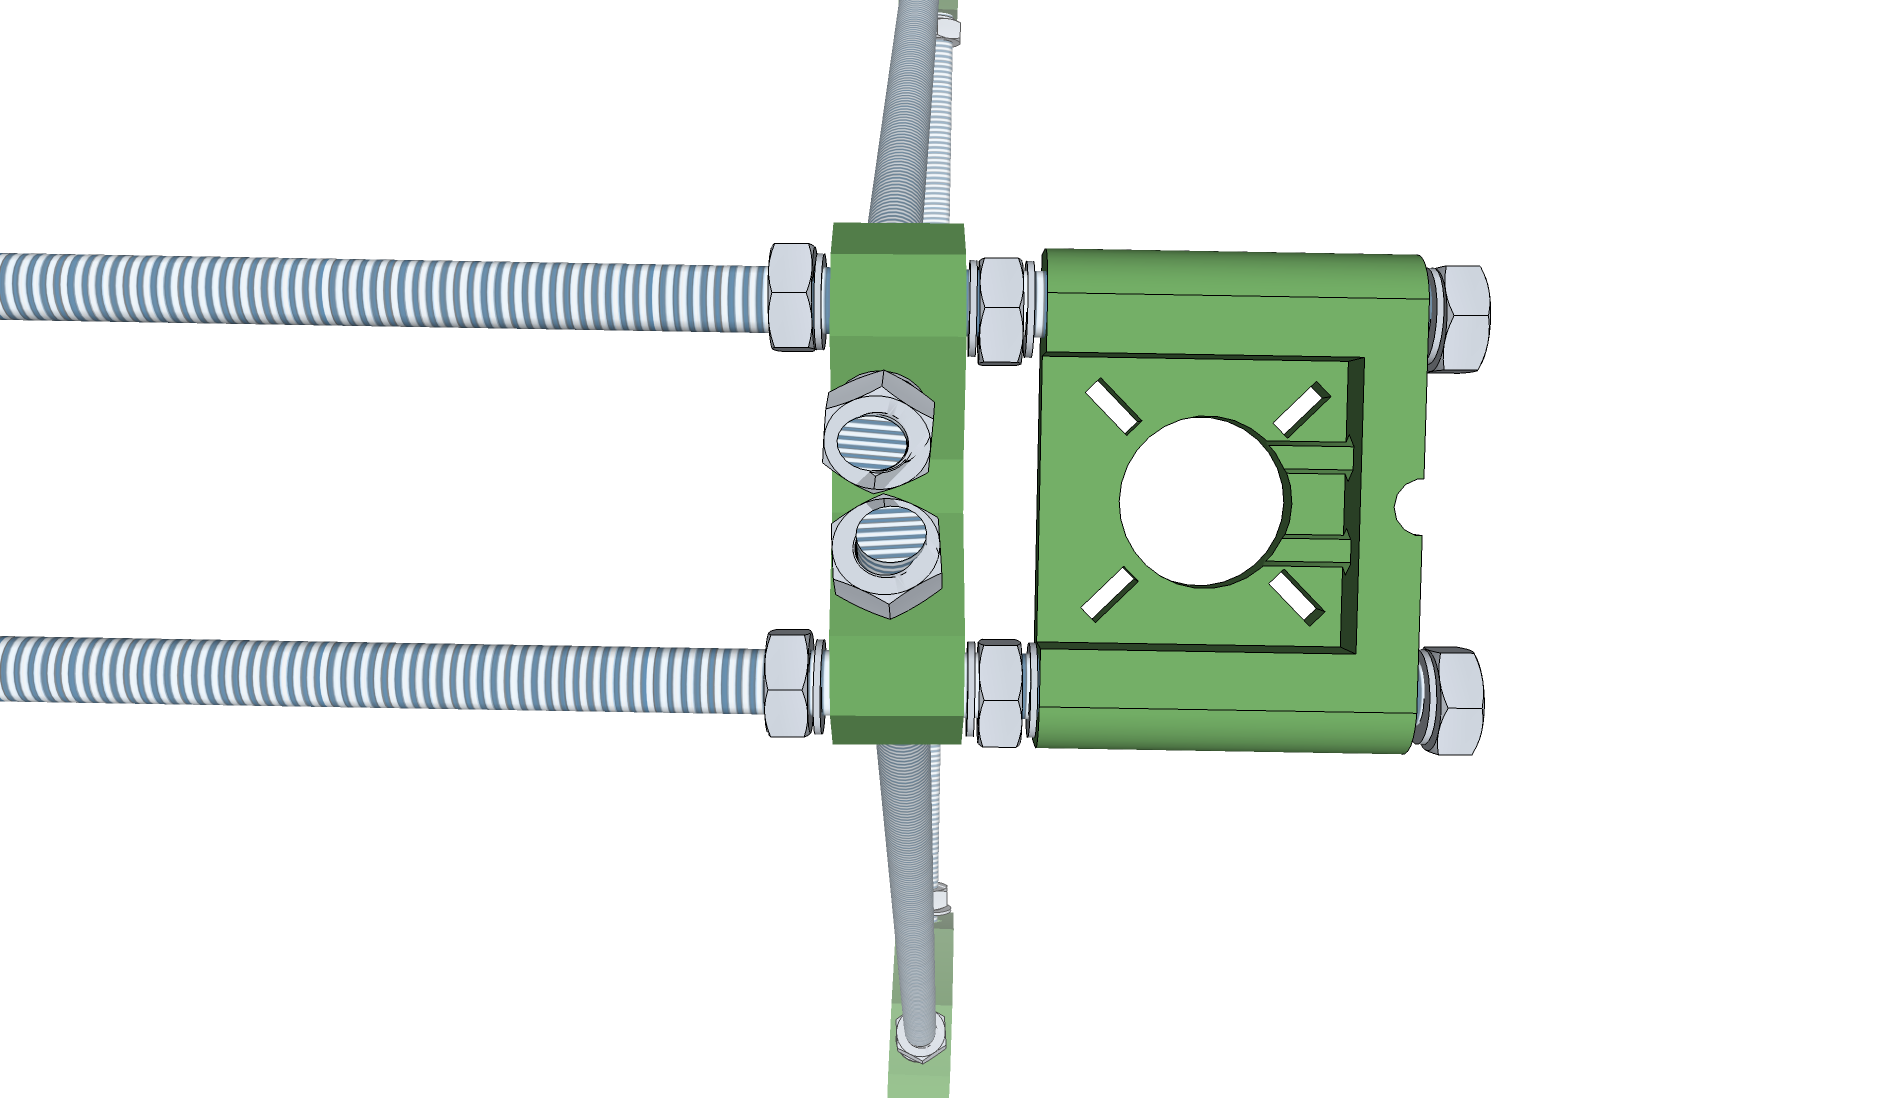
\includegraphics[width=1\linewidth]{graphics/ch4_5_2.png}
	
	\section{}
	Repeat this on the other side.\\
	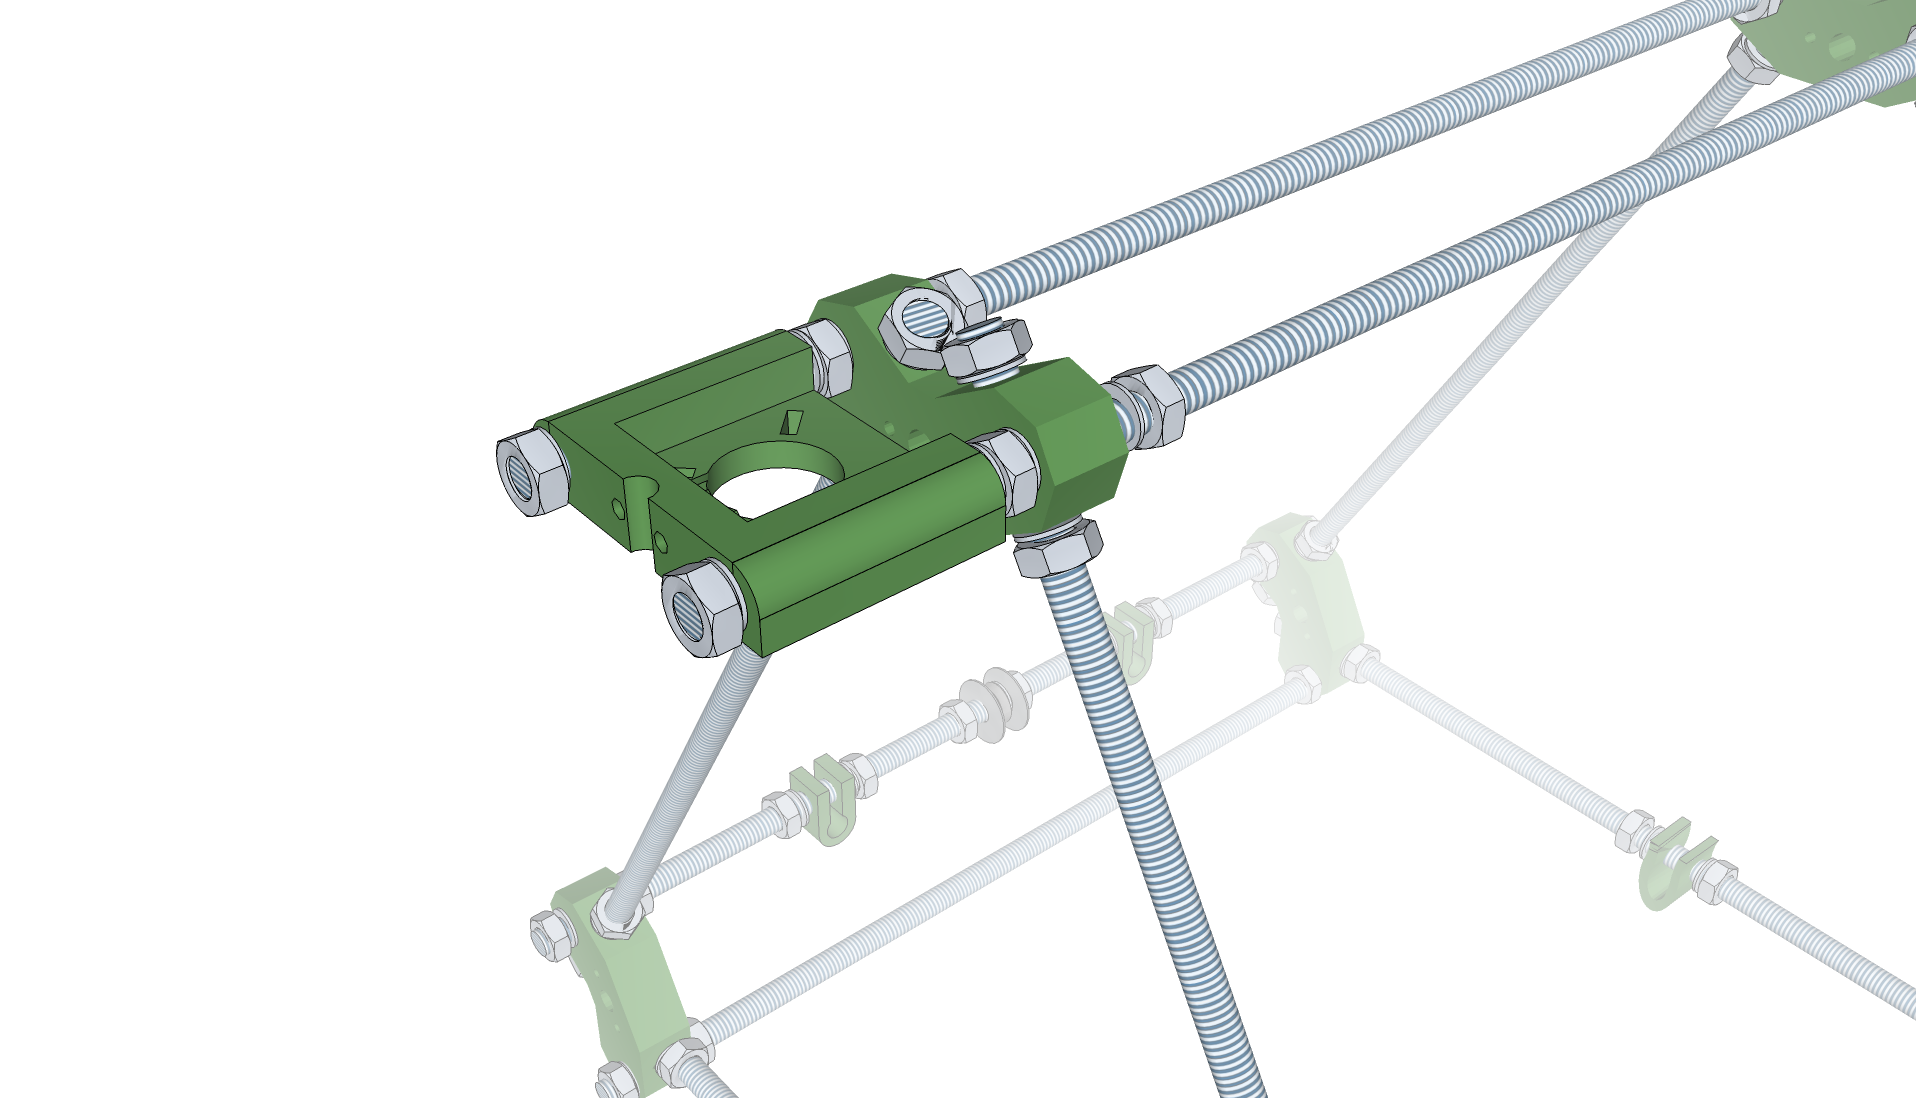
\includegraphics[width=1\linewidth]{graphics/ch4_6_1.png}
	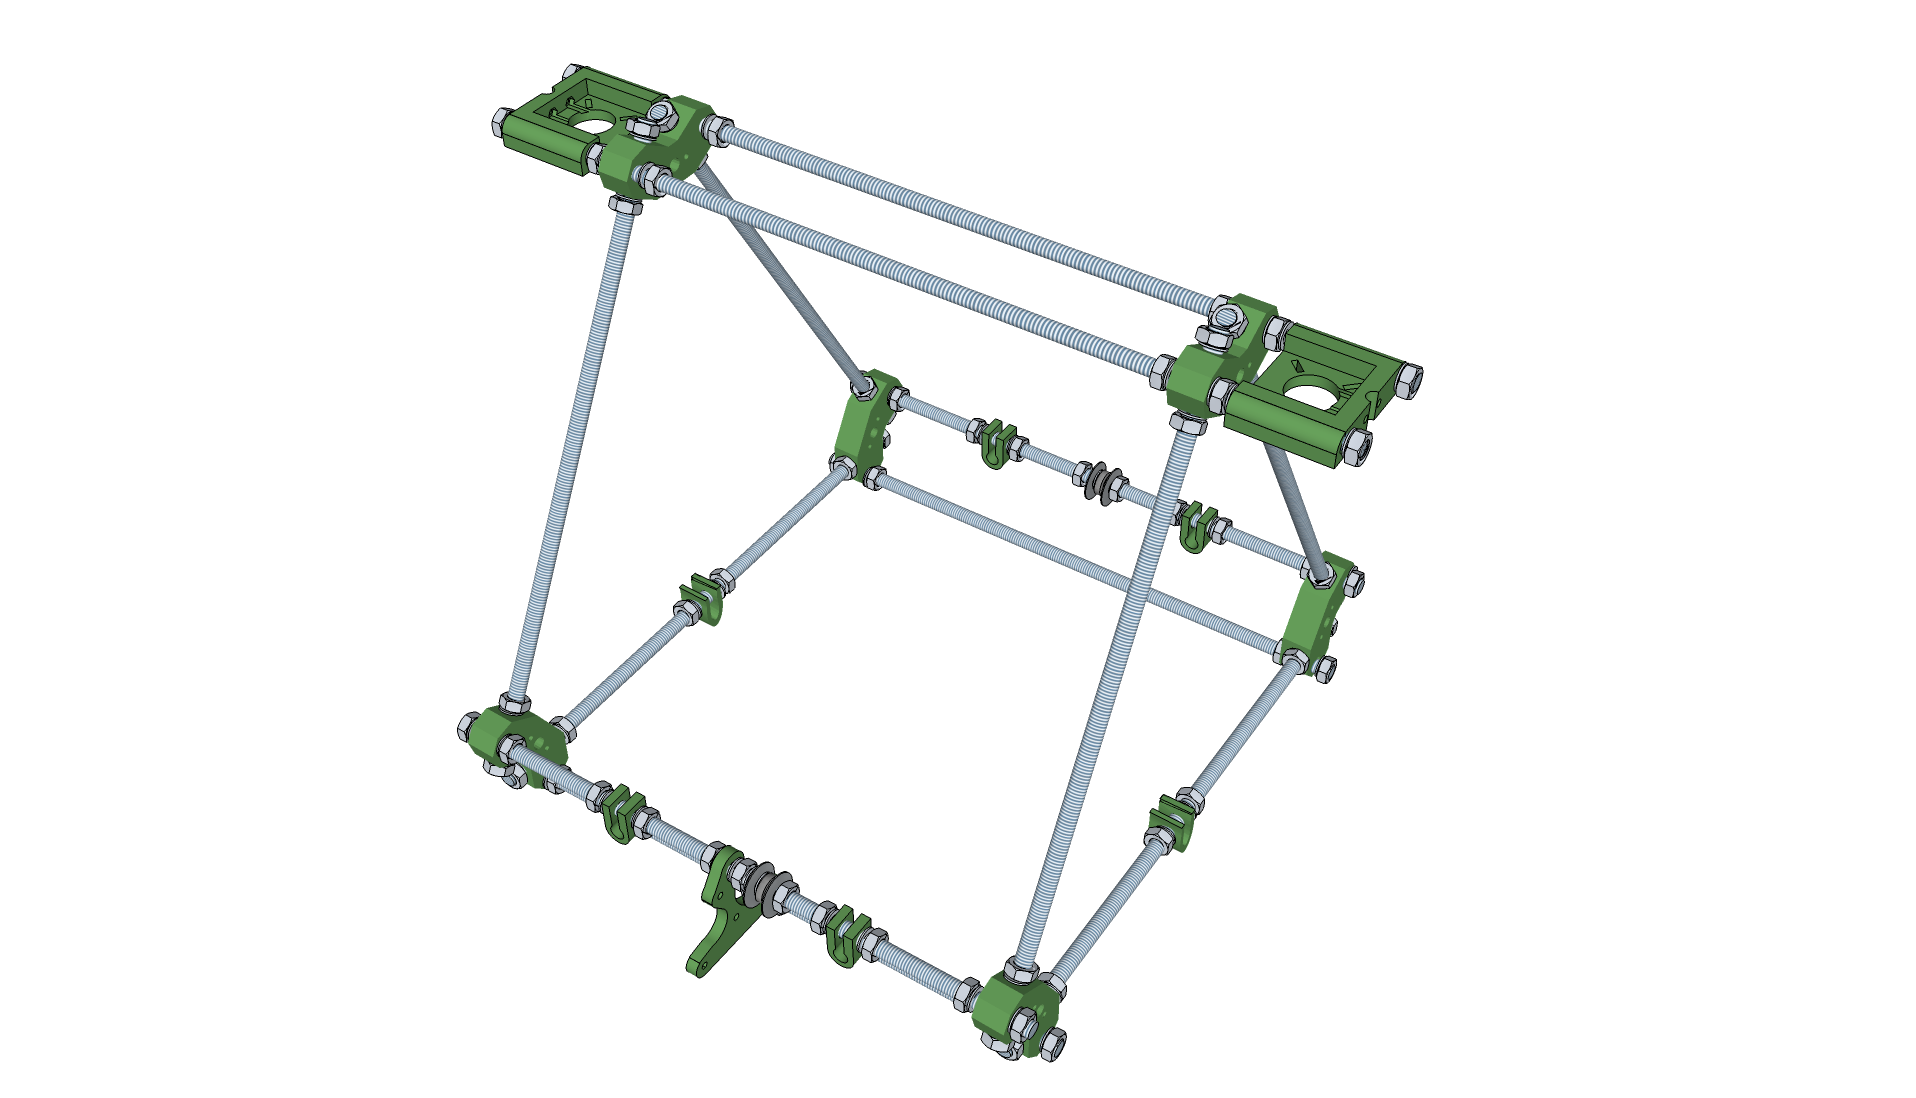
\includegraphics[width=1\linewidth]{graphics/ch4_6_2.png}
	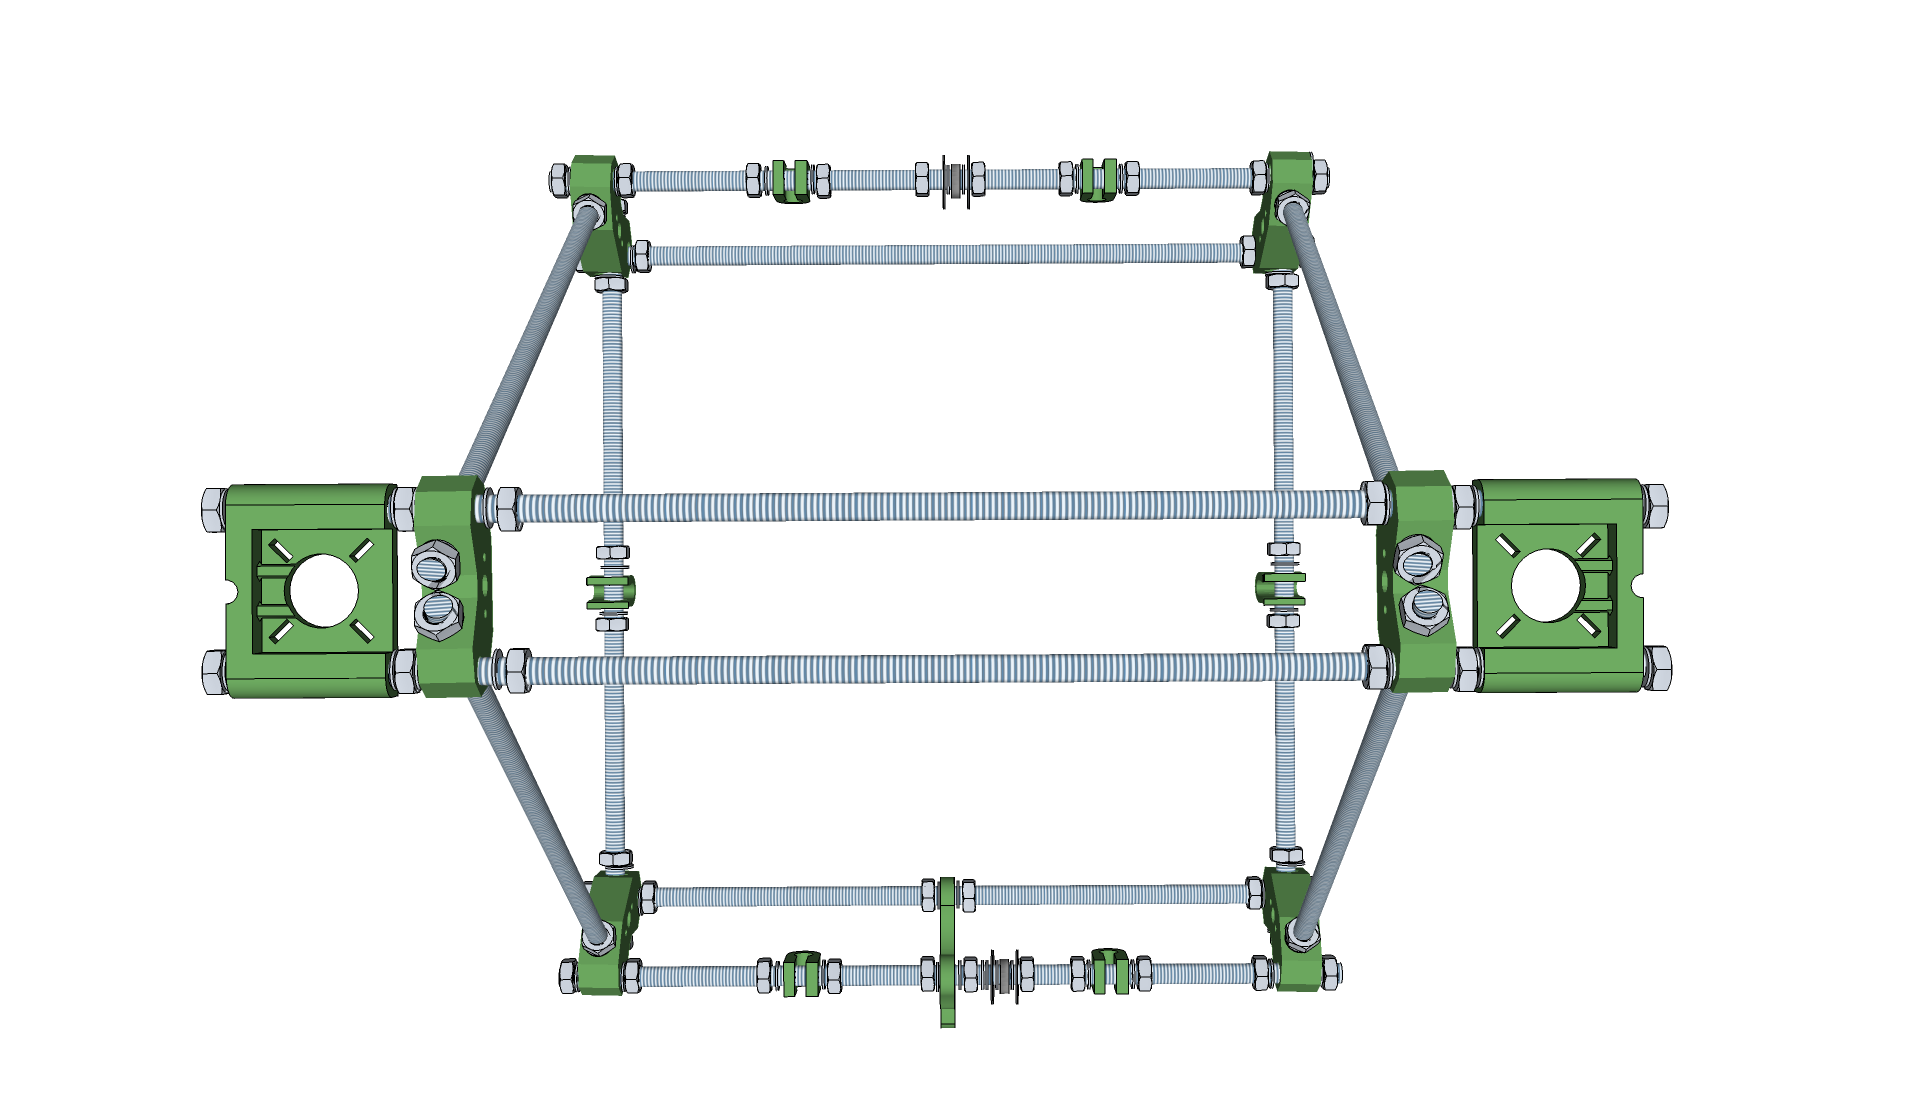
\includegraphics[width=1\linewidth]{graphics/ch4_6_3.png}
	
	\chapter{Tightening the frame}
	
	\section{}
	Verify that the triangle vertices have distance J1 (290mm, equivalent is 11-13/32") from plastic to plastic
	along each of the three sides. Once you are sure of this, tighten the outer vertex nuts until they are
	firmly attached and unable to move, but do not crush the plastic parts.\\
	\includegraphics[width=1\linewidth]{graphics/ch5_1.png}
	
	\section{}
	Adjust each of the bottom rods until it has distance J2 (234mm, equivalent is 9-7/32") between the
	inside ends of the vertices. Use frame jig J2 to check this if you have it. Once you are sure this is true,
	tighten the outer vertex nuts until they are firm, but do not crush the plastic.\\
	\includegraphics[width=1\linewidth]{graphics/ch5_2.png}
	
	\section{}
	Adjust the top of the frame so that the distance between the inside ends of the vertices is precisely J2
	(234mm, equivalent is 9-7/32") and the length of rod outside the vertex on one side is the same as the
	length outside the vertex on the other side. Double-check the distances before tightening the nut on the
	outside of the vertex.\\
	\includegraphics[width=1\linewidth]{graphics/ch5_3.png}
	
	\section{}
	The frame should now be fairly stable. Using a plumb line or similar (for example a nut hanging on a
	length of yarn), adjust the bar clamps on the bottom side of each triangle until they are close to center
	of the top vertices. Do not tighten the nuts either side of the bar clamps yet. These need to space the
	440 mm rod exactly 1 bar clamp from the center line of the bot. This is so the polished z-rods are
	exactly centered with the bot and run perfectly vertical.\\
	\includegraphics[width=1\linewidth]{graphics/ch5_4.png}
	
	\section{}
	Insert the 440mm threaded rod through the two bar clamps on the bottom of the frame. Make sure the
	new rod is on top of the triangle bottom rod. Adjust it so that the same length sticks out on each side.\\
	\includegraphics[width=1\linewidth]{graphics/ch5_5.png}
	
	\section{}
	On each side, place a nut, washer, bar clamp (threaded through the holes), washer, and another nut.
	The hole to which should go the z-running smooth rod should be virtually in center of bottom triangle
	rods.\\
	\includegraphics[width=1\linewidth]{graphics/ch5_6_1.png}
	\includegraphics[width=1\linewidth]{graphics/ch5_6_2.png}
	\includegraphics[width=1\linewidth]{graphics/ch5_6_3.png}
	[ View from Below ]
	
	\chapter{Assembling the y axis}
	
	\section{}
	Mark each of the four corners of the print bottom plate 8mm (equivalent is ~5/16") from each side with
	the marker.\\
	\includegraphics[width=1\linewidth]{graphics/ch6_1.png}
	
	\section{}
	Carefully drill a 3mm hole in each of the four corners.\\
	\includegraphics[width=1\linewidth]{graphics/ch6_2.png}
	
	\section{}
	Clamp the print bottom plate and the print top plate together, so that the bottom plate is equally far from
	each edge of the top plate. Drill 3mm holes into the top plate through the corner holes in the bottom
	plate so that they match on both plates.\\
	\includegraphics[width=1\linewidth]{graphics/ch6_3_1.png}
	\includegraphics[width=1\linewidth]{graphics/ch6_3_2.png}
	
	\section{}
	Slide the two 406mm smooth rods through the bar clamps on the front and rear threaded rods. They
	should fit snugly and be approximately parallel.\\
	\includegraphics[width=1\linewidth]{graphics/ch6_4.png}
	
	\section{}
	Place the narrow side of the "print bottom" plate between the rods. This ensures they are exactly
	140mm (equivalent is 5-33/64") apart from each other. Adjust the nuts on the front side bar clamps until
	the print bottom plate just barely fits between the rods. Try to get them at an approximately equal
	distance from the middle of the rod.\\
	\includegraphics[width=1\linewidth]{graphics/ch6_5.png}
	
	\section{}
	Tighten the front nuts just enough that they do not move on their own, but no further.\\
	\includegraphics[width=1\linewidth]{graphics/ch6_6.png}
	
	\section{}
	Measure the distance from the left front vertex to the left smooth rod. Adjust the distance from the left
	rear vertex to the left smooth rod to match it. This ensures the left rod is parallel to the frame. Tighten
	the nuts on the left clamp just enough that they do not move around.\\
	\includegraphics[width=1\linewidth]{graphics/ch6_7_1.png}
	\includegraphics[width=1\linewidth]{graphics/ch6_7_2.png}
	
	\section{}
	Place the print bottom plate next to the left smooth rod on the rear side. Adjust the right rear bar clamp's
	nuts until the narrow side of the bottom plate barely fits between the rods.\\
	\includegraphics[width=1\linewidth]{graphics/ch6_8.png}
	
	\section{}
	Recheck the distances from the left vertex to the left rod are the same at the front and rear and that the
	short side of the print bottom plate fits snugly between the smooth rods both at the front and at the rear.
	This should ensure that the rods are parallel to each other and to the frame.\\
	\includegraphics[width=1\linewidth]{graphics/ch6_9.png}
	
	\section{}
	Tighten the nuts on all of the four bar clamps now.\\
	\includegraphics[width=1\linewidth]{graphics/ch6_10.png}
	
	\section{}
	Snap 2 PLA bushings\index{bushings} onto each of the two smooth rods. Place them about 120mm apart on each rod.
	Make sure they slide freely on the rods. Put a dab of glue on the top side of the bushings\index{bushings} (the side
	opposite the open side). Carefully place the print bottom plate on top of the bushings\index{bushings}, so that it's equally
	far apart from each of the two triangles (see diagram below). Wait for the glue to dry.\\
	\includegraphics[width=1\linewidth]{graphics/ch6_11_1.png}
	\includegraphics[width=1\linewidth]{graphics/ch6_11_2.png}
	
	\section{}
	While the glue is drying, adjust the bearing on the rear threaded rod until it is exactly across from the
	front threaded rod. Tighten the nuts on the y motor bracket and the bearings at this point. All nuts on the
	front and rear rods should now be tight.\\
	\includegraphics[width=1\linewidth]{graphics/ch6_12.png}
	
	\section{}
	Also while the glue is drying, ensure that the hole in the center of the pulley matches your motor shaft (it
	should slide on and fit very snugly). If it is too tight to fit, drill it out.\\
	\includegraphics[width=1\linewidth]{graphics/ch6_13.png}
	
	\section{}
	Insert an M3 nut into the rectangular slot on the pulley bottom. You may need to widen the slot slightly
	to do this. Make sure that the center of the nut is aligned with the channel in the pulley that goes to the
	center hole.\\
	\includegraphics[width=1\linewidth]{graphics/ch6_14_1.png}
	\includegraphics[width=1\linewidth]{graphics/ch6_14_2.png}
	\includegraphics[width=1\linewidth]{graphics/ch6_14_3.png}
	
	\section{}
	Once you are satisfied with the position of the nut, insert an M3 grub screw into the channel on the rim
	of the hub. Tighten it until you see the end of the screw inside the center hole. Then unscrew it enough
	to slide the pulley onto the motor shaft.\\
	\includegraphics[width=1\linewidth]{graphics/ch6_15_1.png}
	\includegraphics[width=1\linewidth]{graphics/ch6_15_2.png}
	\includegraphics[width=1\linewidth]{graphics/ch6_15_3.png}
	
	\section{}
	Place the motor with the pulley on it next to the mounting holes in the y motor bracket. Position the
	motor the left, so that the pulley ends up on the side of the bearing.\\
	\includegraphics[width=1\linewidth]{graphics/ch6_16.png}
	
	\section{}
	Adjust the pulley position on the shaft so that when the motor is flush with the bracket, the teeth on the
	pulley are approximately at the position of the bearing.\\
	\includegraphics[width=1\linewidth]{graphics/ch6_17.png}
	
	\section{}
	Fasten the motor with 3 M3x10 bolts. Put a washer between each bolt and the y motor bracket.\\
	\includegraphics[width=1\linewidth]{graphics/ch6_18.png}
	
	\section{}
	Tighten the grub screw so that the pulley cannot move along the shaft.\\
	\includegraphics[width=1\linewidth]{graphics/ch6_19.png}
	
	\section{}
	Position the y belt on top of the print bottom plate and through both of the bearings. Pull lightly on both
	ends so that it is straight. If the belt is not straight, adjust the position of the rear bearing until it is. 		Use a marker to mark out the position of the belt on the print bottom plate. Also mark which side of the plate 		is on the left.\\
	\includegraphics[width=1\linewidth]{graphics/ch6_20_1.png}
	\includegraphics[width=1\linewidth]{graphics/ch6_20_2.png}
	
	\section{}
	After the glue has dried, carefully pop the print bottom plate with the PLA bushings\index{bushings} off the rails. Place
	the two belt clamps perpendicular to the marked position of the belt, several centimeters apart. Make
	sure the belt position is between the two holes on each clamp. Use a marker to mark where the holes of
	the belt clamps would be on the plate.\\
	\includegraphics[width=1\linewidth]{graphics/ch6_21.png}
	
	\section{}
	Carefully drill a 3mm hole through each of the four marked belt clamp holes.\\
	\includegraphics[width=1\linewidth]{graphics/ch6_22.png}
	
	\section{}
	Place the print bottom plate back on the smooth rods, paying attention to the marking to make sure the
	correct side is on the left.\\
	\includegraphics[width=1\linewidth]{graphics/ch6_23.png}
	
	\section{}
	Place one end of the belt, toothed side down, where the holes for the front belt clamp are. Put a washer
	onto each of two M3x25 bolts, and thread them through the holes in one of the belt clamps. Then attach
	the clamp to the top of the plate, clamping down the belt. Leave several centimeters of the belt behind
	the clamp.\\
	\includegraphics[width=1\linewidth]{graphics/ch6_24_1.png}
	\includegraphics[width=1\linewidth]{graphics/ch6_24_2.png}
	
	\section{}
	Put two M3 nuts underneath the plate and thread them onto the bolts. Tighten both nuts so that the end
	of the belt is firmly attached to the plate, toothed side down.\\
	\includegraphics[width=1\linewidth]{graphics/ch6_25.png}
	
	\section{}
	Pass the belt over the front bearing, around the motor pulley, and then up underneath the plate to the
	other bearing. Pull it tight, then lay it on top of the plate, toothed side down.\\
	\includegraphics[width=1\linewidth]{graphics/ch6_26.png}
	
	\section{}
	Put a washer onto each of two M3x25 bolts, and thread them through the holes in the second belt
	clamp. Then attach the clamp to the top of the plate, clamping down the belt.\\
	\includegraphics[width=1\linewidth]{graphics/ch6_27.png}
	
	\section{}
	Attach an M3 nut to each of the two bolts, and pull the belt tight before tightening the two nuts.\\
	\includegraphics[width=1\linewidth]{graphics/ch6_28.png}
	
	\section{}
	Turn the motor by hand. It should turn with little effort, and each slight rotation should be matched by a
	slight movement of the plate. Make sure it slides smoothly along the entire length of the rods. Pushing
	the plate should immediately make the motor turn. Make sure the belt is not too loose (plate and motor
	should not be able to move independently) or too tight (taking a lot of effort to move the plate). Once
	you are confident your belt tension is correct, tighten the clamps very firmly. You may now trim the belt,
	but leave several centimeters behind each clamp for future adjustment.\\
	\includegraphics[width=1\linewidth]{graphics/ch6_29.png}
	
	\chapter{Assembling the X axis}
	Drill out the center hole in the hexagonal section of the x-end-idler and x-end-motor parts to 8mm.\\
	\includegraphics[width=1\linewidth]{graphics/ch7_1.png}
	
	\section{}
	Take the x-end-idler. Check the size of the hole on the flat, thin side surface. If it is 4mm in diameter,
	enlarge it using a file until it's 8mm in diameter.\\
	\includegraphics[width=1\linewidth]{graphics/ch7_2.png}
	
	\section{}
	Place 4 M3 nuts in the nut traps in the long channels on the bottom of the x-end-idler. You may find
	pulling them into the nut trap using an M3 bolt makes it easier. Thread M3x10 bolts through them, but
	just far enough that they do not fall out.\\
	\includegraphics[width=1\linewidth]{graphics/ch7_3_1.png}
	\includegraphics[width=1\linewidth]{graphics/ch7_3_2.png}
	\includegraphics[width=1\linewidth]{graphics/ch7_3_3.png}
	\includegraphics[width=1\linewidth]{graphics/ch7_3_4.png}
	
	\section{}
	Place 4 M3 nuts in the nut traps of the x-end-motor part as well. Thread M3x10 bolts through those as
	above.\\
	\includegraphics[width=1\linewidth]{graphics/ch7_4.png}
	
	\section{}
	Place the x-end-motor and x-end-idler 50cm apart, so that the hexagonal parts are facing each other.\\
	\includegraphics[width=1\linewidth]{graphics/ch7_5.png}
	
	\section{}
	Slide the two 495mm smooth rods into the x-end idler. Make sure they go past the nut traps.\\
	\includegraphics[width=1\linewidth]{graphics/ch7_6.png}
	
	\section{}
	Slide the other ends of the rods into x-end-motor. Make sure they go past the nut traps. The hexagonal
	sections of the motor and idler should still be facing each other.\\
	\includegraphics[width=1\linewidth]{graphics/ch7_7_1.png}
	\includegraphics[width=1\linewidth]{graphics/ch7_7_2.png}
	
	\section{}
	Tighten the M3 bolts on the x-end-idler. The x-end-motor should be able to move along the rods with
	minor effort. Do not tighten the x-end-motor bolts yet.\\
	\includegraphics[width=1\linewidth]{graphics/ch7_8.png}
	
	\section{}
	Thread an M8 nut onto one end of the 50mm threaded rod. (Alternatively, you can use an M8x50 bolt)
	\includegraphics[width=1\linewidth]{graphics/ch7_9.png}
	
	\section{}
	Put the following parts in this order onto the free end of the threaded rod (behind the nut): 1 fender
	washer, 1 M8 washer, 1 608 bearing, 1 M8 washer, 1 fender washer.\\
	\includegraphics[width=1\linewidth]{graphics/ch7_10.png}
	
	\section{}
	Thread the free end of the threaded rod into the side of the x-end-idler. The bearing should be on the
	outside. Put an M8 washer and an M8 nut on the inside and tighten both nuts.\\
	\includegraphics[width=1\linewidth]{graphics/ch7_11_1.png}
	\includegraphics[width=1\linewidth]{graphics/ch7_11_2.png}
	
	\chapter{Assembling the Z axis}
	
	\section{}
	Use a spirit level to make sure the two rods at the top of the frame are horizontal. If they are not, stack
	bits of paper under the vertices at the bottom until they are.\\
	\includegraphics[width=1\linewidth]{graphics/ch8_1.png}

	\section{}
	Drop a plumb line (or a nut tied to a length of yarn) directly down from the indentation on the side of the
	left z-motor-holder. Adjust the two bar clamps at the bottom of the frame on the left side until the nut
	falls into the U of the outer clamp. Repeat on the other side.\\
	\includegraphics[width=1\linewidth]{graphics/ch8_2.png}
	
	\section{}
	Put M3 nuts into the nut traps on both z-motor-holder ends.\\
	\includegraphics[width=1\linewidth]{graphics/ch8_3.png}
	
	\section{}
	Put an M3 washer on 2 M3x25 bolts and thread them into the flat (non-indented) end of a rod-clamp.
	Attach the rod-clamp to one of the z-motor-holders. Do not tighten.\\
	\includegraphics[width=1\linewidth]{graphics/ch8_4.png}
	
	\section{}
	Repeat for the other z-motor-holder and rod-clamp.\\
	\includegraphics[width=1\linewidth]{graphics/ch8_5_1.png}
	The M3x25 bolts are too long for the recent Prusa z-motor-holder and rod-clamp, and using round
	headed bolts as shown above will result in the shaft of the bolt interfering with the seating of the z-
	motor. One could either use shorter bolts (approx. M3x20), or cut the M3x25's to size.\\
	\includegraphics[width=1\linewidth]{graphics/ch8_5_2.png}	
	\includegraphics[width=1\linewidth]{graphics/ch8_5_3.png}	
	An alternative is to use hexagonal bolts, and insert them in reverse with the shaft pointing outwards.\\
	\includegraphics[width=1\linewidth]{graphics/ch8_5_4.png}
	\includegraphics[width=1\linewidth]{graphics/ch8_5_5.png}
	
	\section{}
	Insert a 330mm smooth rod into the space between each z-motor-holder and rod-clamp. Slide it in from
	the top. On the bottom, insert it into the U of the bottom bar clamp.\\
	\includegraphics[width=1\linewidth]{graphics/ch8_6_1.png}
	\includegraphics[width=1\linewidth]{graphics/ch8_6_2.png}
	\includegraphics[width=1\linewidth]{graphics/ch8_6_3.png}
	
	\section{}
	Using the plumb line, check that the smooth rods are vertical. If they are not, adjust the bottom bar
	clamp positions until they are. This is critical, so take as much time as you need.\\
	\includegraphics[width=1\linewidth]{graphics/ch8_7.png}
	
	\section{}
	Tighten the nuts on the bar clamps and the bolts on the rod clamps. Check again with the plumb line.\\
	\includegraphics[width=1\linewidth]{graphics/ch8_8.png}
	
	\section{}
	Place two PLA bushings\index{bushings} on each of the smooth rods. Make sure they slide freely.\\
	\includegraphics[width=1\linewidth]{graphics/ch8_9.png}
	
	\section{}
	Position the x-axis assembly inside the frame so that the bushing channels on the x-axis-motor and x-
	axis-idler align with the bushings\index{bushings}. The x-end-idler should be on the right, with the bearing on the rear
	side of the machine.\\
	\includegraphics[width=1\linewidth]{graphics/ch8_10_1.png}
	\includegraphics[width=1\linewidth]{graphics/ch8_10_2.png}
	\includegraphics[width=1\linewidth]{graphics/ch8_10_3.png}
	
	\section{}
	Put a blob of glue on the flat side of each bushing.\\
	\includegraphics[width=1\linewidth]{graphics/ch8_11.png}
	
	\section{}
	Push the rectangular channels of x-end-idler and x-end-motor against the flat of the bushings\index{bushings}. Position
	the x-end-idler against the bushings\index{bushings} on the right side of the machine and then slide the x-end-motor
	along the x-axis smooth rods until it makes contact with the bushings\index{bushings} on the left side of the machine.
	Let the glue dry.\\
	\includegraphics[width=1\linewidth]{graphics/ch8_12_1.png}
	\includegraphics[width=1\linewidth]{graphics/ch8_12_2.png}
	
	\section{}
	While the glue is drying, assemble the couplings. Insert an M3x25 bolt, with an M3 washer, through
	each of the two side holes on each coupling. Put an M3 washer and M3 nut on the other end. Do not
	tighten yet.\\
	\includegraphics[width=1\linewidth]{graphics/ch8_13_1.png}
	\includegraphics[width=1\linewidth]{graphics/ch8_13_2.png}
	\includegraphics[width=1\linewidth]{graphics/ch8_13_3.png}
	Note: The M3x25 bolts are a little too long for the couplings, and restrict the
	vertical movement of the x-chassis, or interfere with the z-axis smooth bars.
	Either use smaller bolts (M3x20), or cut the M3x25's to size.
	
	\section{}
	Once the glue has dried, slide the X axis to the top of the Z axis smooth rod, and place some kind of support 		underneath the x-axis smooth rods to hold it up in approximately the middle of the frame.
	Tighten the M3x10 screws on the bottom of the x-end-motor.\\
	\includegraphics[width=1\linewidth]{graphics/ch8_14_1.png}
	\includegraphics[width=1\linewidth]{graphics/ch8_14_2.png}
	
	\section{}
	Slide X axis to the bottom of the Z axis smooth rod, if you feel the
	bushings\index{bushings} binding, jog the bar clamps on both sides of the Z axis untill
	the bushings\index{bushings} can travel the full length of the Z rod with no resistance.\\
	\includegraphics[width=1\linewidth]{graphics/ch8_15.png}
	
	\section{}
	Insert an M8 nut into the bottom of the hexagonal channel of x-end-motor. Repeat for x-end-idler.\\
	\includegraphics[width=1\linewidth]{graphics/ch8_16.png}
	
	\section{}
	(optional) Insert a spring into the top of the hexagonal channel of each x-end part. Insert an M8 nut on
	top of each spring.\\
	\includegraphics[width=1\linewidth]{graphics/ch8_17_1.png}
	\includegraphics[width=1\linewidth]{graphics/ch8_17_2.png}
	
	\section{}
	Thread one end of the 210mm threaded rods into each hexagonal channel from above, compressing
	the top nut and spring if you have them. The threaded rod should turn freely in each channel, and the
	nuts should stay snugly in place. Turn the rods until about half their length sticks out from the bottom of
	the parts.\\
	\includegraphics[width=1\linewidth]{graphics/ch8_18_1.png}
	\includegraphics[width=1\linewidth]{graphics/ch8_18_2.png}
	
	\section{}
	Place a NEMA 17 motor into each of the two z-motor-holder parts, shaft down. You
	may optionally fasten them from underneath with M3x10 bolts and M3 washers.\\
	\includegraphics[width=1\linewidth]{graphics/ch8_19_1.png}	
	Note: You might not want to secure the z-motors if you have wobbling issues with you x-axis. This is
	especially true if your threaded rods are not straight.\\
	\includegraphics[width=1\linewidth]{graphics/ch8_19_2.png}
	\includegraphics[width=1\linewidth]{graphics/ch8_19_3.png}
	\includegraphics[width=1\linewidth]{graphics/ch8_19_4.png}
	
	\section{}
	Attach the narrower end of a coupling to each of the motor shafts. Do not tighten the nuts on the
	coupling yet.\\
	\includegraphics[width=1\linewidth]{graphics/ch8_20_1.png}
	\includegraphics[width=1\linewidth]{graphics/ch8_20_2.png}
	
	\section{}
	Turn the 210mm threaded rods so that they go upwards and enter the coupling. Screw them as far into
	the coupling as they will go, but do not use excessive force.\\
	\includegraphics[width=1\linewidth]{graphics/ch8_21.png}
	
	\section{}
	Carefully tighten the M3 nuts on both couplings.\\
	\includegraphics[width=1\linewidth]{graphics/ch8_22.png}
	
	\section{}
	Turn both threaded rods so that the X axis moves up. Make sure the couplings are supporting the
	weight. If the Z axis rods are hard to turn, or one is a lot harder to turn than the other, you will need to
	clean the inside of the spring track. The best way I have found to do this is put a nut on the end of a
	long scrap piece of threaded rod. Heat the nut up on your stove on high. then take the nut and run it up
	and down the inside of the spring chamber till the walls are smooth, and a little bigger than the nut that
	goes it. This should loosen up the hole enough that once reassembled the trouble side travels
	smoothly.\\
	\includegraphics[width=1\linewidth]{graphics/ch8_23.png}
	
	\section{}
	Place a spirit level on the x-axis smooth rods. Turn the threaded rod on one side only until the X axis is
	level. Your Z axis is ready.\\
	\includegraphics[width=1\linewidth]{graphics/ch8_24_1.png}
	\includegraphics[width=1\linewidth]{graphics/ch8_24_2.png}
	
	\chapter{Installing the x carriage}

	\section{}
	Ensure that the hole in the center of the pulley matches your motor shaft (it should slide on and fit very
	snugly). If it is too tight to fit, drill it out.\\
	\includegraphics[width=1\linewidth]{graphics/ch9_1.png}
	
	\section{}
	Insert an M3 nut into the rectangular slot on the pulley bottom. You may need to widen the slot slightly
	to do this. Make sure that the center of the nut is aligned with the channel on the side of the pulley rim.\\
	\includegraphics[width=1\linewidth]{graphics/ch9_2.png}
	
	\section{}
	Once you are satisfied with the position of the nut, insert an M3 grub screw into the channel on the rim
	of the hub. Tighten it until you see the end of the screw inside the center hole. Then unscrew it enough
	to slide the pulley onto the motor shaft.\\
	\includegraphics[width=1\linewidth]{graphics/ch9_3.png}
	
	\section{}
	Slide the pulley onto the motor shaft so that the rim comes onto the shaft last. Leave 1mm or so of shaft
	between the pulley and the motor body. Tighten the grub screw.\\
	\includegraphics[width=1\linewidth]{graphics/ch9_4.png}
	
	\section{}
	Insert the motor into the x-end-motor part so that the motor body is on the front of the machine and the
	pulley points towards the rear. The pulley teeth and the idler on the opposite side of the X axis should
	be aligned.\\
	\includegraphics[width=1\linewidth]{graphics/ch9_5_1.png}
	\includegraphics[width=1\linewidth]{graphics/ch9_5_2.png}
	\includegraphics[width=1\linewidth]{graphics/ch9_5_3.png}	
	Note: The x-axis smooth rods can occupy the space where the motor should go.
	If this is the case: loosen the screws holding the x-end-motor and x-end-idler parts to
	the x-axis smooth rod, and push through the smooth rod until it sits flush on the motor
	side.
	
	\section{}
	Fasten the motor using 4 M3x10 bolts and 4 M3 washers. The motor body should now be on top of the
	x-axis smooth rods.\\
	\includegraphics[width=1\linewidth]{graphics/ch9_6_1.png}
	\includegraphics[width=1\linewidth]{graphics/ch9_6_2.png}
	
	\section{}
	Place 4 PLA bushings\index{bushings} on the x-axis smooth rods. Make sure they slide freely.\\
	\includegraphics[width=1\linewidth]{graphics/ch9_7.png}
	
	\section{}
	Put a blob of glue on the flat side of each bushing.\\
	\includegraphics[width=1\linewidth]{graphics/ch9_8.png}
	
	\section{}
	Place the x-carriage on top of the bushings\index{bushings}, making sure they fit into the channels. The protruding part
	of the x-carriage with the four nut traps should be on the side of the pulley and idler, pointing towards
	the rear of the machine.\\
	\includegraphics[width=1\linewidth]{graphics/ch9_9_1.png}
	\includegraphics[width=1\linewidth]{graphics/ch9_9_2.png}
	
	\section{}
	Wait for the glue to dry.\\
	\includegraphics[width=1\linewidth]{graphics/ch9_10.png}
	
	\section{}
	Once the glue has dried, make sure the carriage can slide along the rods freely from end to end. Turn
	the entire frame around so that the rear of the machine faces towards you.\\
	\includegraphics[width=1\linewidth]{graphics/ch9_11.png}
	
	\section{}
	Put an M3 washer on each of two M3x25 bolts. Thread them through the holes of one belt-clamp.
	Repeat for the second belt-clamp.\\
	\includegraphics[width=1\linewidth]{graphics/ch9_12.png}
	
	\section{}
	Loosely attach one of the belt clamps to the carriage. Thread the two bolts through the holes in the
	carriage and attach nuts to them. Make sure there is enough space for the belt to slide between the
	clamp and the carriage. Repeat for the other clamp.\\
	\includegraphics[width=1\linewidth]{graphics/ch9_13_1.png}
	\includegraphics[width=1\linewidth]{graphics/ch9_13_2.png}
	
	\section{}
	Slide one end of the belt through the left clamp, toothed side up. Pull several centimeters through, then
	tighten the clamp.\\
	\includegraphics[width=1\linewidth]{graphics/ch9_14_1.png}
	\includegraphics[width=1\linewidth]{graphics/ch9_14_2.png}
	
	\section{}
	Run the belt over the 608 bearing and the motor pulley, then thread it through the other clamp, toothed
	side up. The belt should now form an elongated loop with the teeth on the inside of the loop. Pull the
	belt tight and tighten the second clamp.\\
	\includegraphics[width=1\linewidth]{graphics/ch9_15_1.png}
	\includegraphics[width=1\linewidth]{graphics/ch9_15_2.png}
	
	\section{}
	Verify that the belt tension is right. Turning the motor pulley by hand should make the carriage move.
	The carriage should move freely along the entire length of the axis.\\
	\includegraphics[width=1\linewidth]{graphics/ch9_16.png}
	
	\section{}
	Use two M4x20 bolts and two M4 nuts to mount the extruder to the x-carriage.\\
	\includegraphics[width=1\linewidth]{graphics/ch9_17_1.png}
	\includegraphics[width=1\linewidth]{graphics/ch9_17_2.png}
	\includegraphics[width=1\linewidth]{graphics/ch9_17_3.png}
	
	\chapter{Wiring the electronics\index{electronics}}

	\section{}
	There are various electronics\index{electronics} configurations out there, but they are mostly compatible. Regardless of
	what electronics\index{electronics} you have, you should have at least three stepper drivers, ideally four. Those are either
	integrated on the board or separate modules. Identify the motor connections for X, Y, Z and the
	extruder stepper (E on some setups). Also identify the connections for the heated bed\index{heated bed} (if you have one),
	the extruder heater connection, the extruder and heated bed\index{heated bed} thermistors, and the X, Y and Z MIN
	endstop connections.\\
	\includegraphics[width=1\linewidth]{graphics/ch10_1.png}
	
	\section{}
	Screw or glue your endstops (opto or microswitch) to the long side of the three endstop holders.\\
	\includegraphics[width=1\linewidth]{graphics/ch10_2.png}	
	[ Note: endstops shown here are indicative only. Please check positions and layout against your own Mendel. ]
	
	\section{}
	If you are using opto endstops, you will need to make three opto flags. These are long, thin strips of
	some easily formable, opaque material, for example metal sheet from drink cans. If you are using
	microswitch endstops, you can skip this step. Take an empty drink can and cut three 10mmx30mm
	pieces from from it. These will be your optoflags.\\
	\includegraphics[width=1\linewidth]{graphics/ch10_3.png}	
	[ Note: Steps for optical endstops shown for completeness. Please double check all steps when using this approach ]
	
	\section{}
	Position your endstops on the smooth rods. Facing the front of the machine, place one on the left z
	smooth rod below where the X axis currently is. This is your Place one on the far left of the rear X axis
	smooth rod. Place the third one on the right y axis smooth rod behind the print bottom plate.\\
	\includegraphics[width=1\linewidth]{graphics/ch10_4_1.png}
	\includegraphics[width=1\linewidth]{graphics/ch10_4_2.png}
	\includegraphics[width=1\linewidth]{graphics/ch10_4_3.png}
	
	\section{}
	Put an M3 washer on an M3x25 bolt and thread it through each endstop holder, and put a washer and
	M3 nut on the other side. Do not tighten these nuts yet.\\
	\includegraphics[width=1\linewidth]{graphics/ch10_5.png}
	
	\section{}
	If you are using opto endstops, glue an optoflag onto the left side of the x-carriage, the bottom of the x-
	motor-bracket (pointing down) and the print bottom plate, so that they go through the gap in the
	optoswitch as the axis slides.\\
	\includegraphics[width=1\linewidth]{graphics/ch10_6_1.png}
	\includegraphics[width=1\linewidth]{graphics/ch10_6_2.png}
	\includegraphics[width=1\linewidth]{graphics/ch10_6_3.png}	
	[ Note: Steps for optical endstops shown for completeness. \\
	Please double check all steps when using this approach ]
	
	\section{}
	You now need to determine the limits of each axis. With the extruder/hotend installed, slide the X
	carriage left until the nozzle is 10mm to the right from the left edge of the print bottom plate. Reposition
	the endstop so that the opto/switch is engaged in this position. If your optoflag is too long, trim it until it
	just barely triggers the endstop when the nozzle is in this position. Tighten the nut on the X endstop,
	being careful not to move it.\\
	\includegraphics[width=1\linewidth]{graphics/ch10_7_1.png}
	\includegraphics[width=1\linewidth]{graphics/ch10_7_2.png}
	\includegraphics[width=1\linewidth]{graphics/ch10_7_3.png}
	[ Top ]
	
	\section{}
	Slide the print bottom plate backwards until the nozzle is about 42mm (equivalent is 1-21/32") in front of
	the front edge of the print bottom plate. Reposition the endstop so that it engages when the print bottom
	plate is in this position. Tighten the Y endstop nut, being careful not to move it.\\
	\includegraphics[width=1\linewidth]{graphics/ch10_8_1.png}
	\includegraphics[width=1\linewidth]{graphics/ch10_8_2.png}
	
	\section{}
	Adjust the Z endstop so that it is triggered when the Z axis moves downwards. Do not worry about the
	height yet. You will need to adjust the position of this endstop once the bed is installed and leveled.\\
	\includegraphics[width=1\linewidth]{graphics/ch10_9.png}
	
	\section{}
	Decide where your electronics\index{electronics} will live. Mount these in place first, that will allow you to route cables
	easier.\\
	\includegraphics[width=1\linewidth]{graphics/ch10_10.png}
	
	\section{}
	Slide the X carriage as far away from the electronics\index{electronics} as possible.\\
	\includegraphics[width=1\linewidth]{graphics/ch10_11.png}
	
	\section{}
	Route the cables from each of the endstops along the frame to the electronics\index{electronics} board. Plug each one
	into the appropriate connector. For the X endstop, leave enough slack in the cable to allow the X axis to
	move along the Z all the way up and down the frame. Make sure none of the wires interfere with the
	movement of the axes. Use zipties to fix the wires to the frame.\\
	\includegraphics[width=1\linewidth]{graphics/ch10_12.png}
	[ Diagram shows general cable locations only. Please follow the instructions and mount the wires
	close to the frame as appropriate. ]
	
	\section{}
	Splice the Z motor wires together in parallel. If the motors are identical, join each wire with the wire of
	the same color, and then attach them to the connector that matches your electronics\index{electronics}. Route the wires
	along the frame to your electronics\index{electronics} board, and attach them to the Z-driver connector. Use cable ties to
	fix the wires to the frame.\\
	\includegraphics[width=1\linewidth]{graphics/ch10_13.png}
	
	\section{}
	Attach the Y motor wires to the connector that matches the electronics\index{electronics}, route them along the frame
	(making sure they don't interfere with the Y-axis movement) and attach them to your electronics\index{electronics} at the
	Y-driver connector. Fix the wires to the frame with zipties.\\
	\includegraphics[width=1\linewidth]{graphics/ch10_14.png}
	
	\section{}
	Attach the X motor wires to the connector that matches the electronics\index{electronics}, route them along the frame and
	attach them to your electronics\index{electronics} at the X-driver connector. Leave enough slack for the X-axis to move all
	the way up and down the Z axis without getting caught on the wires. Fix the wires to the frame with
	zipties.\\
	\includegraphics[width=1\linewidth]{graphics/ch10_15.png}
	
	\section{}
	Leaving enough slack so that the wires don't get stretched even when the X carriage is furthest away
	from the electronics\index{electronics}, route the extruder motor, heater, and thermistor wires along the frame, to the
	electronics\index{electronics}. Keep careful track of which wire is which. Color-coding is recommended. If your wires are
	not different colors, attach labels to the ends. Attach connectors to the wires to match your electronics\index{electronics}
	and plug them into your electronics\index{electronics} board. The stepper connection goes into the EXTRUDER/E
	connector. Tie the cables down to the frame with zipties.\\
	\includegraphics[width=1\linewidth]{graphics/ch10_16.png}
	
	\section{}
	Move the X and Y axes all the way in each direction, and check that no wires interfere with movement.
	Once done, slide each axis to approximately the middle of its range.\\
	\includegraphics[width=1\linewidth]{graphics/ch10_17.png}
	
	[ The following steps have no suitable visual counterpart and so are given as found on the wiki. ]
	
	\section{}
	Get a piece of paper, and write "X, Y, Z, E" on it.
	
	\section{}
	Plug in the power and USB connections to the electronics\index{electronics}. From this point on, if ANYTHING acts
	strange, switch off power first, and figure it out later. This is extremely important!
	
	\section{}
	Connect to the electronics\index{electronics} from a computer using repsnapper, reprap host, or replicatorg.
	
	\section{}
	Stand in front of the machine. In the software, tell the X axis to move forward (positive) by 10mm. If it
	moves to the RIGHT, write "OK" under X on your paper. If it moves to the LEFT, write "REV" under X. If
	it does not move write "NO" under it.
	
	\section{}
	Tell the Y axis to move forward (positive) by 10mm. If it moves FORWARD (towards you), write "OK"
	under Y. If it moves BACKWARD (away from you), write "REV" under Y. If the axis does not move,
	write "NO" under Y on your paper.
	
	\section{}
	Tell the Z axis to move forward (positive) by 10mm. If it moves UP, write "OK" under Z. If it moves
	DOWN, write "REV" under Z. If the axis does not move, write "NO" under Z on your paper.
	
	\section{}
	Tell the extruder to move forward (positive). If it moves in the direction that would push filament into the 		nozzle, write "OK" under Z. If it moves in the opposite direction, write "REV" under Z. If the axis
	does not move, write "NO" under Z on your paper.
	
	\section{}
	Close the software and switch off the power to the machine!
	
	\section{}
	For each axis that is labeled "REV", unplug its connector from the electronics\index{electronics}, turn it by 180 degrees,
	and plug it in again. If the connector is polarized (can only be plugged in one way), you might need to
	reconnect the wires to the connector.
	
	\section{}
	For each axis that is labeled "NO", make sure its connector is wired to the motor, and the connector is
	seated properly.
	
	\section{}
	Repeat the test until all axes are labeled "OK". Now tell the X and Y axes to home. They should move
	until they reach their endstops, then stop.
	
	\chapter{Attaching the print bed}
	
	\section{}
	If you have a heated build platform, install it on the print top plate at this point. Cover your top plate or
	build platform with whatever your build surface material will be (Kapton, blue tape, etc.)
	\includegraphics[width=1\linewidth]{graphics/ch11_1.png}
	
	\section{}
	Put a washer on each of the four M3x40 bolts.\\
	\includegraphics[width=1\linewidth]{graphics/ch11_2.png}
	
	\section{}
	Thread each bolt through one of the holes in the print top plate.\\
	\includegraphics[width=1\linewidth]{graphics/ch11_3.png}
	
	\section{}
	Put an M3 washer, a ballpoint pen spring, and another M3 washer onto each bolt.\\
	\includegraphics[width=1\linewidth]{graphics/ch11_4_1.png}
	\includegraphics[width=1\linewidth]{graphics/ch11_4_2.png}
	\includegraphics[width=1\linewidth]{graphics/ch11_4_3.png}
	
	\section{}
	Thread a nut onto each bolt to fasten it to the print top plate. Do not tighten. This nut is only there to
	hold the springs in place.\\
	\includegraphics[width=1\linewidth]{graphics/ch11_5_1.png}
	\includegraphics[width=1\linewidth]{graphics/ch11_5_2.png}
	
	\section{}
	Carefully place the print top plate on top of the print bottom plate. Make sure each bolt goes through
	one of the holes in the print bottom plate.\\
	\includegraphics[width=1\linewidth]{graphics/ch11_6_1.png}
	\includegraphics[width=1\linewidth]{graphics/ch11_6_2.png}
	
	\section{}
	Put an M3 washer and nut on the end of each of the bolts.\\
	\includegraphics[width=1\linewidth]{graphics/ch11_7.png}
	
	\section{}
	Level the bed. To do this, put a spirit level on top of the bed and adjust the nuts of each of the M3 bolts
	until the spirit level shows the bed is level. Use the top nut to adjust the height and the bottom nut to fix
	it. If you have a heated build platform, put the spirit level on the platform. Once done, tighten all nuts.\\
	\includegraphics[width=1\linewidth]{graphics/ch11_8.png}
	
	\section{}
	Adjust the Z endstop so that it is triggered when the nozzle is just
	barely above the bed.\\
	\includegraphics[width=1\linewidth]{graphics/ch11_9.png}
	
	\section{}
	You are now ready to print. Enjoy!\\
	\includegraphics[width=1\linewidth]{graphics/ch11_10.png}
	
	\printindex
\end{document}
